\documentclass[a4paper,11pt]{article}
\pdfminorversion=4
\usepackage{amsmath}
\usepackage{amsthm}
\usepackage{amsfonts}
\usepackage{mathrsfs}
\usepackage{amssymb}
\usepackage{mathpazo}
\usepackage[dvipsnames]{xcolor}
\usepackage{bm}
\usepackage[no-weekday]{eukdate}
\usepackage[bb=boondox]{mathalfa}
\usepackage{paralist}
\usepackage{natbib}
\usepackage{url}
\usepackage[textwidth=6.25in,textheight = 10in]{geometry}
\usepackage{placeins}
\usepackage[hidelinks]{hyperref}
\usepackage{multirow, float}
\usepackage{makecell}
\usepackage{calc}
\usepackage{graphicx}
\usepackage{enumitem}
\usepackage{microtype}
\usepackage{todonotes}
\usepackage{caption}
\DeclareCaptionStyle{italic}[justification=centering]
 {labelfont={bf},textfont={it},labelsep=colon}
\captionsetup[figure]{style=italic,singlelinecheck=true}
\captionsetup[table]{style=italic,singlelinecheck=true}

\setlength{\parskip}{0cm}
\setlength{\parindent}{1em}
\usepackage[compact]{titlesec}
\titlespacing{\section}{0pt}{2ex}{1ex}
\titlespacing{\subsection}{0pt}{1ex}{0ex}
\titlespacing{\subsubsection}{0pt}{0.5ex}{0ex}
\usepackage{titling}\pretitle{\begin{center}\LARGE\bfseries}
\usepackage[bottom,hang,flushmargin]{footmisc}
\usepackage{adjustbox}

\def\sectionautorefname{Section}
\def\subsectionautorefname{Section}

%% LINE AND PAGE BREAKING
\sloppy
\allowdisplaybreaks
\clubpenalty = 10000
\widowpenalty = 10000
\brokenpenalty = 10000

% NOTE: To produce blinded version, replace "0" with "1" below.
\newcommand{\blind}{1}

%\usepackage{setspace}
\usepackage{caption}
\captionsetup[figure]{labelfont={bf}, font = small, singlelinecheck=true}
\captionsetup[table]{labelfont={bf}, font = small, singlelinecheck=true}
\usepackage{subcaption}

\DeclareMathOperator*{\argmin}{arg\,min}
\usepackage{longtable}
\usepackage{booktabs}
\usepackage{array}
\newcolumntype{M}[1]{>{\centering\arraybackslash}m{#1}}
\newcolumntype{L}[1]{>{\raggedright\arraybackslash}m{#1}}
\newcolumntype{R}[1]{>{\raggedleft\arraybackslash}m{#1}}

\newcommand{\alphavet}{\bm{\alpha}}
\newcommand{\betavet}{\bm{\beta}}
\newcommand{\epsvet}{\bm{\varepsilon}}
\newcommand{\etavet}{\bm{\eta}}
\newcommand{\lambdavet}{\bm{\lambda}}
\newcommand{\Unovet}{\bm{1}}
\newcommand{\avet}{\bm{a}}
\newcommand{\bvet}{\bm{b}}
\newcommand{\cvet}{\bm{c}}
\newcommand{\dvet}{\bm{d}}
\newcommand{\evet}{\bm{e}}
\newcommand{\pvet}{\bm{p}}
\newcommand{\fvet}{\bm{f}}
\newcommand{\tvet}{\bm{t}}
\newcommand{\uvet}{\bm{u}}
\newcommand{\vvet}{\bm{v}}
\newcommand{\wvet}{\bm{w}}
\newcommand{\xvet}{\bm{x}}
\newcommand{\yvet}{\bm{y}}
\newcommand{\zvet}{\bm{z}}
\newcommand{\Avet}{\bm{A}}
\newcommand{\Bvet}{\bm{B}}
\newcommand{\Cvet}{\bm{C}}
\newcommand{\Dvet}{\bm{D}}
\newcommand{\Evet}{\bm{E}}
\newcommand{\Fvet}{\bm{F}}
\newcommand{\Gvet}{\bm{G}}
\newcommand{\Hvet}{\bm{H}}
\newcommand{\Ivet}{\bm{I}}
\newcommand{\Jvet}{\bm{J}}
\newcommand{\Kvet}{\bm{K}}
\newcommand{\Lvet}{\bm{L}}
\newcommand{\Mvet}{\bm{M}}
\newcommand{\Nvet}{\bm{N}}
\newcommand{\Pvet}{\bm{P}}
\newcommand{\Qvet}{\bm{Q}}
\newcommand{\Rvet}{\bm{R}}
\newcommand{\Svet}{\bm{S}}
\newcommand{\Tvet}{\bm{T}}
\newcommand{\Uvet}{\bm{U}}
\newcommand{\Wvet}{\bm{W}}
\newcommand{\Xvet}{\bm{X}}
\newcommand{\Yvet}{\bm{Y}}
\newcommand{\Zvet}{\bm{Z}}
\newcommand{\Zerovet}{\bm{0}}
\newcommand{\Omegavet}{\bm{\Omega}}
\newcommand{\Sigmavet}{\bm{\Sigma}}
\newcommand{\phivet}{\bm{\phi}}

\definecolor{mybluehl}{HTML}{cbd3ff}

% theorem
\makeatletter
\def\@endtheorem{\endtrivlist}
\makeatother

%% tikz
%% Packages to draw hierarchies
\usepackage{tikz}
\usepackage{forest}

\usetikzlibrary{arrows,shapes,positioning,shadows,trees}
\usetikzlibrary{matrix, decorations.pathreplacing, arrows, calc, fit, arrows.meta, decorations.pathmorphing, decorations.markings}

\tikzset{
  basic/.style  = {draw, text width=2cm, drop shadow, font=\sffamily, rectangle},
  root/.style   = {basic, rounded corners=2pt, thin, align=center,
                   fill=green!30},
  level 2/.style = {basic, rounded corners=6pt, thin,align=center, fill=green!60,
                   text width=4em},
  level 3/.style = {basic, thin, align=left, fill=pink!60, text width=1.5em}
}
\newcommand{\relation}[3]
{
	\draw (#3.south) -- +(0,-#1) -| ($ (#2.north) $)
}
\newcommand{\relationW}[2]
{
	\draw (#2.west) -| ($ (#1.north) $)
}
\newcommand{\relationE}[2]
{
	\draw (#2.east) -| ($ (#1.north) $)
}

\newcommand{\relationD}[3]
{
	\draw (#3.east) -- +(#1,0) |- (#2.west)
}

\pgfdeclareimage[height=0.85cm]{ngreen}{fig/boot/ngreen.pdf}
\pgfdeclareimage[height=0.85cm]{nblue}{fig/boot/nblue.pdf}
\pgfdeclareimage[height=0.85cm]{nred}{fig/boot/nred.pdf}
\pgfdeclareimage[height=0.85cm]{nblack}{fig/boot/nblack.pdf}

\theoremstyle{definition}
\newtheorem{definition}{Definition}[section]
\newtheorem{theorem}{Theorem}[section]

% Title page
\makeatletter
\newcommand{\maketitleblind}{\begingroup%
\if1\blind
{
\maketitle
}\fi

\if0\blind
{
\begin{center}%
  \let \footnote \thanks
    {\LARGE \@title \par}%
    \vskip 1.5em%
    {\large \@date}%
  \end{center}
  \bigskip
} \fi
\endgroup}
\makeatother

% Authors code
\usepackage[affil-it, blocks]{authblk}
\setlength{\affilsep}{0em}
\newcommand{\email}[1]{\affil{Email: {\upshape\href{mailto:#1}{#1}}}}
\renewcommand\Affilfont{\itshape\normalsize}

% Abstract code
\makeatletter
\renewenvironment{abstract}{%
    \if@twocolumn
      \section*{\abstractname}%
    \else %
      \begin{center}%
        {\bfseries \large\abstractname\vspace{\z@}}%
      \end{center}%
      \quotation
    \fi}
    {\if@twocolumn\else\endquotation\fi}
\makeatother

%% Title page
%\makeatletter  
%\newcommand{\maketitleblind}{\begingroup%
%\if1\blind
%{
%\clearpage\maketitle
%\thispagestyle{empty}
%\vfill
%%\vskip2cm
%%\noindent\textit{\large\textbf{Preliminary Working Draft}}\\
%%\noindent\textbf{Please do not quote or cite without authors' permission}
%\vfill
%\newpage
%\setcounter{page}{1}
%}\fi
%
%\if0\blind
%{
%\begin{center}%
%  \let \footnote \thanks
%    {\LARGE \@title \par}%
%    \vskip 1.5em%
%    {\large \@date}%
%  \end{center}
%  \bigskip
%} \fi
%\endgroup}
%\makeatother
%
%% Authors code
%\usepackage[affil-it]{authblk}
%\setlength{\affilsep}{0em}
%\newcommand{\email}[1]{\affil{Email: {\upshape\href{mailto:#1}{#1}}}}
%\renewcommand\Affilfont{\itshape\normalsize}
%  
%% Abstract code
%\makeatletter
%\renewenvironment{abstract}{%
%    \if@twocolumn
%      \section*{\abstractname}%
%    \else %
%      \begin{center}%
%        {\bfseries \large\abstractname\vspace{\z@}}%
%      \end{center}%
%      \quotation
%    \fi}
%    {\if@twocolumn\else\endquotation\fi}
%\makeatother

%% Settings
\title{\bf Cross-temporal Probabilistic Forecast Reconciliation: Appendix}
\author{Daniele Girolimetto}
\affil{Department of Statistical Sciences, University of Padova}
\email{daniele.girolimetto@phd.unipd.it}
\author{George Athanasopoulos}
\affil{Department of Econometrics and Business Statistics, Monash University}
\email{george.athanasopoulos@monash.edu}
\author{Tommaso Di Fonzo}
\affil{Department of Statistical Sciences, University of Padova}
\email{tommaso.difonzo@unipd.it}
\author{Rob J Hyndman}
\affil{Department of Econometrics and Business Statistics, Monash University}
\email{rob.hyndman@monash.edu}

\begin{document}

\def\spacingset#1{\renewcommand{\baselinestretch}{#1}\small\normalsize}
\spacingset{1.1}
  
\maketitleblind

\spacingset{1.3}
\tableofcontents
\newpage
%\listoftables
\appendix
\renewcommand{\thetable}{\Alph{section}.\arabic{table}}
\renewcommand{\thefigure}{\Alph{section}.\arabic{figure}}

\section{Cross-sectional, temporal and cross-temporal covariance approximations}\label{app:covapp}

\autoref{tab:cov_app} presents some approximations for the cross-sectional \citep{hyndman2011, hyndman2016, wickramasuriya2019} and the temporal \citep{athanasopoulos2017, nystrup2020} covariance matrices. \cite{difonzo2023} consider the following approximations for the cross-temporal covariance matrix.
\begin{itemize}[nosep, leftmargin=!, labelwidth=\widthof{ oct$(bdsam)$ -}, align=right]
	\item[oct$(ols)$ -] identity: $\Omegavet_{ct} = \Ivet_{n(k^*+m)}$.
	\item[oct$(struc)$ -] structural: $\Omegavet_{ct} = \mathrm{diag}(\Svet_{ct} \mathbf{1}_{mn_b})$.
	\item[oct$(wlsv)$ -] series variance scaling: $\Omegavet_{ct} = \widehat{\Omegavet}_{ct,wlsv}$, a straightforward extension of the series variance scaling matrix presented by \cite{athanasopoulos2017}.
	\item[oct$(bdshr)$ -] block-diagonal shrunk cross-covariance scaling: $\Omegavet_{ct} = \Pvet\widehat{\Wvet}^{BD}_{ct,shr}\Pvet'$, with $\widehat{\Wvet}^{BD}_{ct,shr}$ a block diagonal matrix where each $k-$block ($k = m,k_{p-1},\dots, 1$) is $\Ivet_{M_k} \otimes \widehat{\Wvet}^{[k]}_{shr}$, $\widehat{\Wvet}^{[k]}_{shr}$ is the shrunk estimate of the cross-sectional covariance matrix proposed by \cite{wickramasuriya2019}, and $\Pvet$ is the commutation matrix such that $\Pvet \mathrm{vec}(\Yvet_{\tau}) = \mathrm{vec}(\Yvet_{\tau}')$.
	\item[oct$(shr)$ -] MinT-shr:   $\Omegavet_{ct} = \hat{\lambda}\widehat{\Omegavet}_{ct,D} + (1-\hat{\lambda})\widehat{\Omegavet}_{ct}$,
	where $\hat{\lambda}$ is an estimated shrinkage coefficient (\citealp{ledoit2004a}), $\widehat{\Omegavet}_{ct,D} = \Ivet_{n(k^\ast + m)} \odot \widehat{\Omegavet}_{ct}$ with $\odot$ denoting the Hadamard product, and $\widehat{\Omegavet}_{ct}$ is the covariance matrix of the cross-temporal one-step ahead in-sample forecast errors.
	\item[oct$(sam)$ -] MinT-sam:  $\Omegavet_{ct} = \widehat{\Omegavet}_{ct}$.
\end{itemize}

 \begin{table}[!h]
 	\centering
 	\footnotesize
 	\begin{tabular}{>{\raggedleft\arraybackslash}m{0.15\linewidth}|>{\centering\arraybackslash}m{0.35\linewidth}|>{\centering\arraybackslash}m{0.35\linewidth}}
 		\toprule
 		                & \textbf{Cross-sectional framework}                                                     & \textbf{Temporal framework}                                                                        \\
 		\midrule
 		identity        & cs$(ols)$: $\Wvet = \Ivet_n$                                                           & te$(ols)$: $\Omegavet = \Ivet_{k^\ast + m}$                                                        \\[0.1cm]
 		structural      & cs$(struc)$: $\Wvet = \mathrm{diag}(\Svet_{cs} \mathbf{1}_{nb})$                       & te$(struc)$: $\Omegavet = \mathrm{diag}(\Svet_{te} \mathbf{1}_{m})$                                \\[0.1cm]
 		series variance & cs$(wls)$: $\Wvet = \widehat{\Wvet}_D = \Ivet_n \odot \widehat{\Wvet}$                 & te$(wlsv)$: $\Omegavet = \widehat{\Omegavet}_{wlsv}$                                               \\[0.1cm]
 		MinT-shr        & cs$(shr)$: $\Wvet = \hat{\lambda}\widehat{\Wvet}_D + (1-\hat{\lambda})\widehat{\Wvet}$ & te$(shr)$: $\Omegavet = \hat{\lambda}\widehat{\Omegavet}_D + (1-\hat{\lambda})\widehat{\Omegavet}$ \\[0.1cm]
 		MinT-sam        & cs$(sam)$: $\Wvet = \widehat{\Wvet}$                                                   & te$(sam)$: $\Omegavet = \widehat{\Omegavet}$                                                       \\
 		\bottomrule \addlinespace[0.1cm]
 		\multicolumn{3}{p{0.9\linewidth}}{\footnotesize \textbf{Note:} $\widehat{\Wvet}$ ($\widehat{\Omegavet}$) is the covariance matrix of the cross-sectional (temporal) one-step ahead in-sample forecast errors, $\widehat{\Omegavet}_{wlsv}$ is a diagonal matrix presented by \cite{athanasopoulos2017}, and $\widehat{\Omegavet}_D = \Ivet_{k^\ast + m} \odot \widehat{\Omegavet}$, where $\odot$ denotes the Hadamard product.}
 	\end{tabular}
 	\caption{Approximations for cross-sectional ($\Wvet$) and temporal ($\Omegavet$) covariance matrices.}
 	\label{tab:cov_app}
\end{table}

\section{Alternative forms of the cross-temporal covariance matrix}\label{app:shr}
In this appendix, some derivations of the solutions proposed in Section 4 to obtain an estimator of the cross-temporal covariance matrix are reported.
Starting from the the definition of cross-temporal covariance matrix we obtain the first equivalence in (10). Therefore, we have that
\begin{align*}
	\lambda \widehat{\Omegavet}_{\textit{hf-bts}, D} &+ (1-\lambda) \widehat{\Omegavet}_{\textit{hf-bts}}\\
	&\Downarrow\\
	\widehat{\Omegavet}_{HB} & = \Svet_{ct}\left[\lambda \widehat{\Omegavet}_{\textit{hf-bts}, D} + (1-\lambda) \widehat{\Omegavet}_{\textit{hf-bts}}\right]\Svet_{ct}'                                                                        \\
	                         & = \lambda \Svet_{ct}\widehat{\Omegavet}_{\textit{hf-bts}, D}\Svet_{ct}'+ (1-\lambda) \Svet_{ct}\widehat{\Omegavet}_{\textit{hf-bts}}\Svet_{ct}'.
\end{align*}
The high-frequency time series representation (the second equivalence) can be derived in the following manner:
\begin{align*}
	\Omegavet & = \Svet_{ct}\Omegavet_{\textit{hf-bts}}\Svet_{ct}'                                                                                                                                                            \\
	          & = \left(\Svet_{cs} \otimes \Svet_{te}\right)\Omegavet_{\textit{hf-bts}}\left(\Svet_{cs} \otimes \Svet_{te}\right)'                                                                                            \\
	          & = \left(\Ivet_n \otimes \Svet_{te}\right)\left(\Svet_{cs} \otimes \Ivet_{m+k^\ast}\right)\Omegavet_{\textit{hf-bts}}\left(\Svet_{cs} \otimes \Ivet_{m+k^\ast}\right)'\left(\Ivet_n \otimes \Svet_{te}\right)' \\
	          & = \left(\Ivet_n \otimes \Svet_{te}\right)\Omegavet_{\textit{hf}}\left(\Ivet_n \otimes \Svet_{te}\right)'
\end{align*}
where $\Omegavet_{\textit{hf}} = \left(\Svet_{cs} \otimes \Ivet_{m+k^\ast}\right)\Omegavet_{\textit{hf-bts}}\left(\Svet_{cs} \otimes \Ivet_{m+k^\ast}\right)'$ and $\Svet_{ct} = \Svet_{cs} \otimes \Svet_{te} = \left(\Ivet_n \otimes \Svet_{te}\right)\left(\Svet_{cs} \otimes \Ivet_{m+k^\ast}\right)$. We can apply the shrinkage estimator as
\begin{align*}
	\lambda \widehat{\Omegavet}_{hf, D} &+ (1-\lambda) \widehat{\Omegavet}_{\textit{hf}}\\
	&\Downarrow\\
	\widehat{\Omegavet}_{H} & = (\Ivet_{n} \otimes \Svet_{te})\left[\lambda \widehat{\Omegavet}_{hf, D} + (1-\lambda) \widehat{\Omegavet}_{\textit{hf}}\right] (\Ivet_{n} \otimes \Svet_{te})'                                                                                                            \\
	                        & = \lambda (\Ivet_{n} \otimes \Svet_{te})\widehat{\Omegavet}_{hf, D}(\Ivet_{n} \otimes \Svet_{te})' + (1-\lambda) (\Ivet_{n} \otimes \Svet_{te})\widehat{\Omegavet}_{\textit{hf}}(\Ivet_{n} \otimes \Svet_{te})'.
\end{align*}
The bottom time series representation (the third equivalence) follows by
\begin{align*}
	\Omegavet & = \Svet_{ct}\Omegavet_{\textit{hf-bts}}\Svet_{ct}'                                                                                                                                                   \\
	          & = \left(\Svet_{cs} \otimes \Svet_{te}\right)\Omegavet_{\textit{hf-bts}}\left(\Svet_{cs} \otimes \Svet_{te}\right)'                                                                                   \\
	          & = \left(\Svet_{cs} \otimes \Ivet_{m+k^\ast}\right)\left(\Ivet_n \otimes \Svet_{te}\right)\Omegavet_{\textit{hf-bts}}\left(\Ivet_n \otimes \Svet_{te}\right)'\left(\Ivet_n \otimes \Svet_{te}\right)' \\
	          & = \left(\Svet_{cs} \otimes \Ivet_{m+k^\ast}\right)\Omegavet_{bts}\left(\Svet_{cs} \otimes \Ivet_{m+k^\ast}\right)',
\end{align*}
where $\Omegavet_{bts} = \left(\Ivet_n \otimes \Svet_{te}\right)\Omegavet_{\textit{hf-bts}}\left(\Ivet_n \otimes \Svet_{te}\right)'$ and $\Svet_{ct} = \Svet_{cs} \otimes \Svet_{te} = \left(\Svet_{cs} \otimes \Ivet_{m+k^\ast}\right)\left(\Ivet_n \otimes \Svet_{te}\right)$. Finally we have that
\begin{align*}
	\lambda \widehat{\Omegavet}_{bts, D} &+ (1-\lambda) \widehat{\Omegavet}_{bts}\\
	&\Downarrow\\
	\widehat{\Omegavet}_{B} & = \left(\Svet_{cs} \otimes \Ivet_{m+k^\ast}\right)\left[\lambda \widehat{\Omegavet}_{bts, D} + (1-\lambda) \widehat{\Omegavet}_{bts}\right]\left(\Svet_{cs} \otimes \Ivet_{m+k^\ast}\right)'                       \\
	                        & = \lambda \left(\Svet_{cs} \otimes \Ivet_{m+k^\ast}\right)\widehat{\Omegavet}_{bts, D}\left(\Svet_{cs} \otimes \Ivet_{m+k^\ast}\right)' +             \\
	                        & \qquad \qquad (1-\lambda) \left(\Svet_{cs} \otimes \Ivet_{m+k^\ast}\right)\widehat{\Omegavet}_{bts}\left(\Svet_{cs} \otimes \Ivet_{m+k^\ast}\right)'.
\end{align*}

In general, the covariance matrix of the reconciled forecasts is equal to $\Mvet \widehat{\Omegavet} \Mvet'$ where $\Mvet = \Svet_{ct}\Gvet$ is the projection matrix. When using the HB approach, the covariance matrix of the reconciliation and the base forecasts will be identical. Indeed, it can be shown (see \citealp{panagiotelis2021} for more details) that if $\Mvet$ is a projection matrix (6) then $\Mvet\Svet_{ct} = \Svet_{ct}\Gvet\Svet_{ct} = \Svet_{ct}$, and we obtain that
\begin{align*}
	\Mvet \widehat{\Omegavet}_{HB} \Mvet' & = \Mvet\Svet_{ct}\widehat{\Omegavet}_{\textit{hf-bts}, HB}\Svet_{ct}'\Mvet'                      \\
	& = \Svet_{ct}\Gvet\Svet_{ct}\widehat{\Omegavet}_{\textit{hf-bts}, HB}\Svet_{ct}'\Gvet'\Svet_{ct}' \\
	& = \Svet_{ct}\widehat{\Omegavet}_{\textit{hf-bts}, HB}\Svet_{ct}' = \widehat{\Omegavet}_{HB}.
\end{align*}

\autoref{fig:num_param} shows the number of parameters for different values of $m$ and $n$, with $n_b$ fixed to approximately $60\%$ of $n$. The right panel reports the boxplot of the percentage reductions in the number of parameters compared to the global approach.
\autoref{fig:shr_grid} gives some visual insights on the covariance matrices obtainable with $\lambda=0$ and $\lambda=1$, respectively, for a simple cross-temporal hierarchical structure with 3 time series and $\mathcal{K}=\{2,1\}$ (e.g, cross-temporal semi-annual, see the Monte Carlo simulation in \autoref{sec:mcsim}).

\begin{figure}[!t]
	\centering
	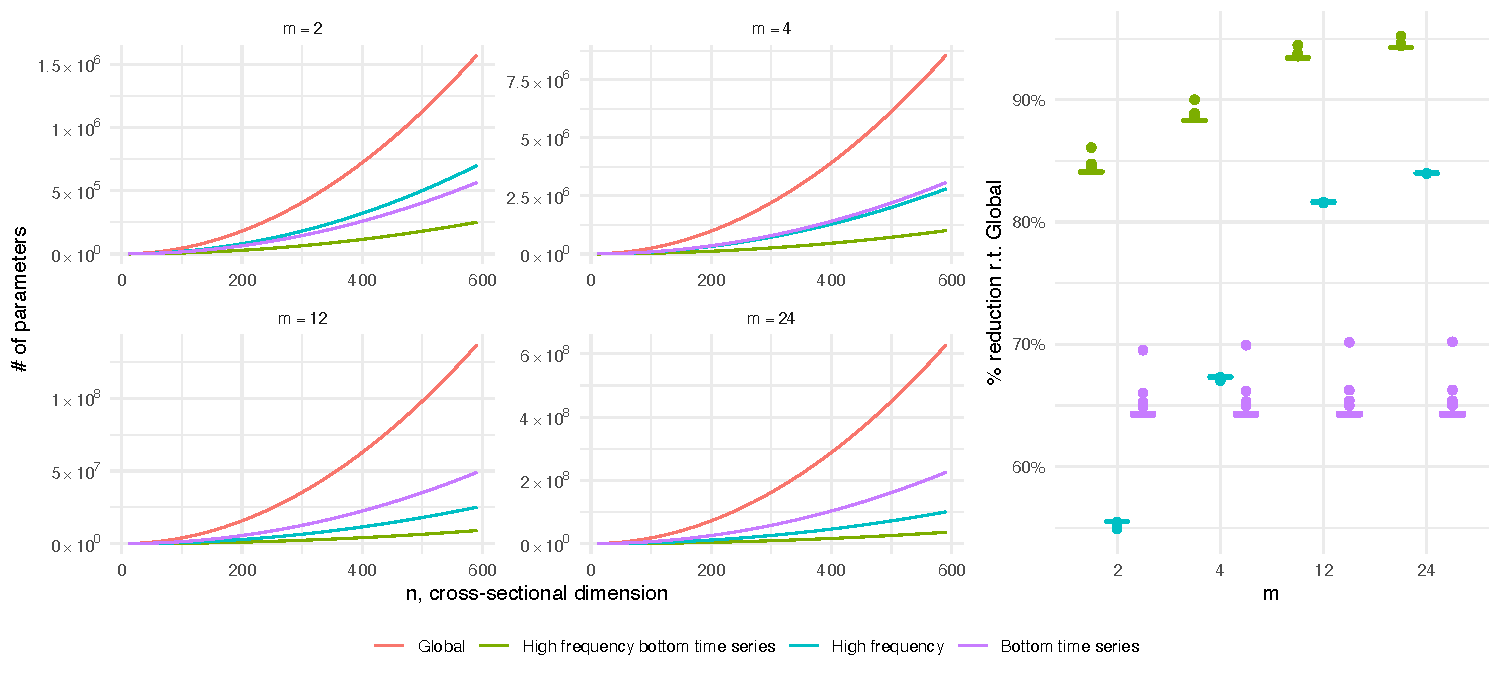
\includegraphics[width = \linewidth]{fig/parameters.pdf}
	\caption{The four graphs on the left represent the number of different parameters in the covariance matrix for the various approaches presented for different values of $m$ and $n$ ($n_b$, the number of bottom time series, is about $60\%$ of the total). On the right, we have the boxplot of the percentage reduction in the number of parameters compared to the global approach.}
	\label{fig:num_param}
\end{figure}

\begin{figure}[!t]
	\centering
	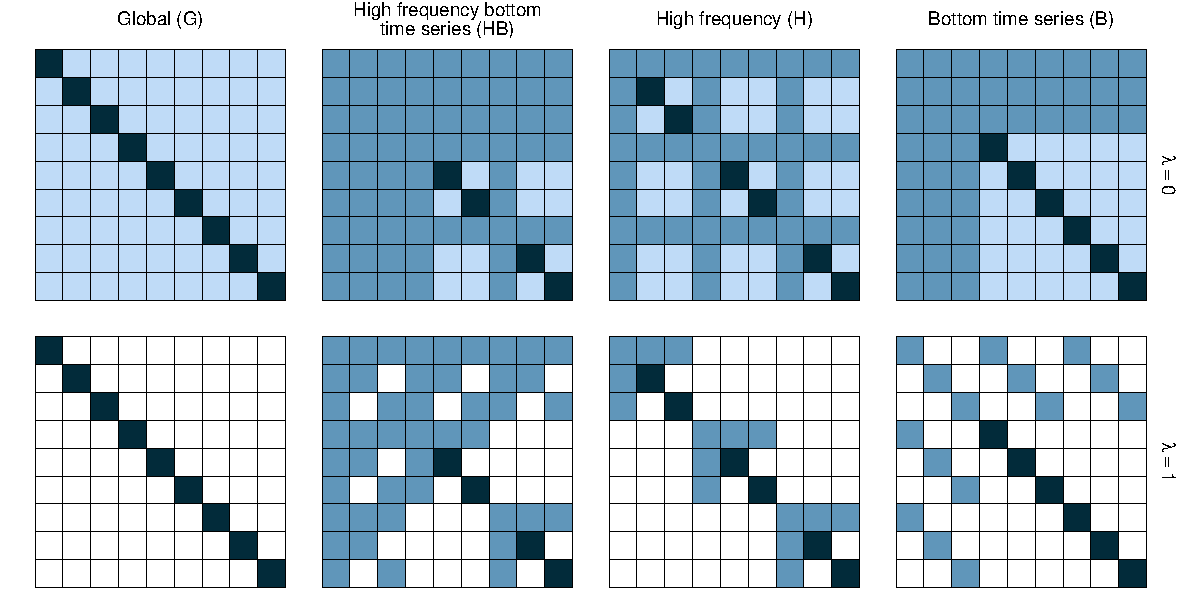
\includegraphics[width = \linewidth]{fig/shr_cov/shr_color.pdf}
	\caption{Representation of four types of covariance matrices that can be obtained from the cross-temporal hierarchical structure ($3$ time series and $m = 2$) for two different values of $\lambda\in\{0,1\}$, the shrinkage parameter. The cells that are not modified by shrinkage are colored black, those actively involved in the shrinkage phase are colored light blue, and those derived from and not estimated by the base forecasts errors are colored blue. Additionally, for $\lambda = 1$, the cells corresponding to a zero value are colored white.}
	\label{fig:shr_grid}
\end{figure}

\section{Monte Carlo simulation}\label{sec:mcsim}

We study the effect of combining cross-sectional and temporal aggregations, using a simple hierarchy that allows us to effectively visualize the quantities involved, such as the covariance matrix. Additionally, the small size and nature of the data generating process make it possible to exactly calculate the true cross-temporal covariance structure, thus providing insights into the nature of the time series data involved in the forecast reconciliation process.

Consider a $2$-level hierarchical structure with three time series (one upper series, $A$, and two bottom series, $B$ and $C$) such that the cross-sectional aggregation matrix is $\Avet_{cs} = \left[ 1 \quad 1 \right]$ ($A = B+C$). The temporal structure we are considering is equivalent to using semi-annual data with $\mathcal{K} = \{2,1\}$ and $m = 2$. The assumed Data-Generating Processes (DPG) for the semi-annual bottom level series are two AR(2) given by
$$
\begin{aligned}
	y_{B,t} &= \phi_{B, 1} y_{B,t-1} + \phi_{B, 2} y_{B,t-2} + \varepsilon_{B, t}\\
	y_{C,t} &= \phi_{C, 1} y_{C,t-1} + \phi_{C, 2} y_{C,t-2} + \varepsilon_{C, t}
\end{aligned}
$$
with parameters\footnote{The $\phivet_B$ and $\phivet_C$ parameters are estimated from the “Lynx" and “Hare" time series contained in the \texttt{pelt} dataset of the \texttt{tsibbledata} package for R \citep{ohara-wild2022}.} $\phivet_B = [\phi_{B,1}\; \phi_{B,2}]' = [1.34\; -0.74]'$ and $\phivet_C  = [\phi_{C,1}\; \phi_{C,2}]' = [0.95\;~-~0.42]'$. The error $\epsvet_t = \left[\varepsilon_{B, t}\quad \varepsilon_{C, t}\right]'$ driving the process is drawn from a multivariate normal distribution with standard deviations simulated from a uniform distribution between 0.5 and 2 and a fixed correlation of -0.8. The cross-sectional error covariance matrix is thus given by
$$
	\Omegavet_{cs} = \begin{bmatrix}
		0.9 & 0   \\
		0   & 1.8
	\end{bmatrix} \begin{bmatrix}
		1    & \rho \\
		\rho & 1
	\end{bmatrix} \begin{bmatrix}
		0.9 & 0   \\
		0   & 1.8
	\end{bmatrix} = \begin{bmatrix}
		\sigma_B^2  & \sigma_{BC} \\
		\sigma_{BC} & \sigma_C^2
	\end{bmatrix}.
$$
To obtain the remaining series, the bottom series are then cross-temporally aggregated.

For the forecast experiment, the base forecasts are computing using AR models where the order is automatically determined by the algorithm proposed by \cite{hyndman2008a} and implemented in the R package \texttt{forecast} \citep{Rforecast}, thus allowing for possible mis-specification in the models. The training window length is 500 years, consisting of 1000 high frequency observations. The experiment is replicated 500 times, with a forecast horizon of 1 year.

Since the AR(2) models used as DPG for the bottom series $B$ and $C$ at the most disaggregated temporal level are known, we may compute the true covariance matrix for one-step ahead forecasts at the annual level $\Omegavet_{ct} = \Svet_{ct}\Omegavet_{\textit{hf-bts}}\Svet_{ct}'$, where
$$
	\Omegavet_{\textit{hf-bts}} = \begin{bmatrix}
		\sigma^2_B            &                                                 &                      &                                        \\
		\phi_{B,1}\sigma_B^2  & \sigma_B^2\left(1+\phi_{B,1}^2\right)           &                      &                                        \\
		\sigma_{BC}           & \phi_{B,1}\sigma_{BC}                           & \sigma_C^2           &                                        \\
		\phi_{C,1}\sigma_{BC} & \sigma_{BC}\left(1+\phi_{B,1}\phi_{C,1} \right) & \phi_{C,1}\sigma_C^2 & \sigma_C^2\left(1+\phi_{C,1}^2\right)\
	\end{bmatrix}.
$$
The detailed calculations can be found in \autoref{app:ar2}.
\autoref{fig:covcorMC} shows both the covariance matrix and the correlation matrix for fixed parameters.

\begin{figure}[!t]
	\centering
	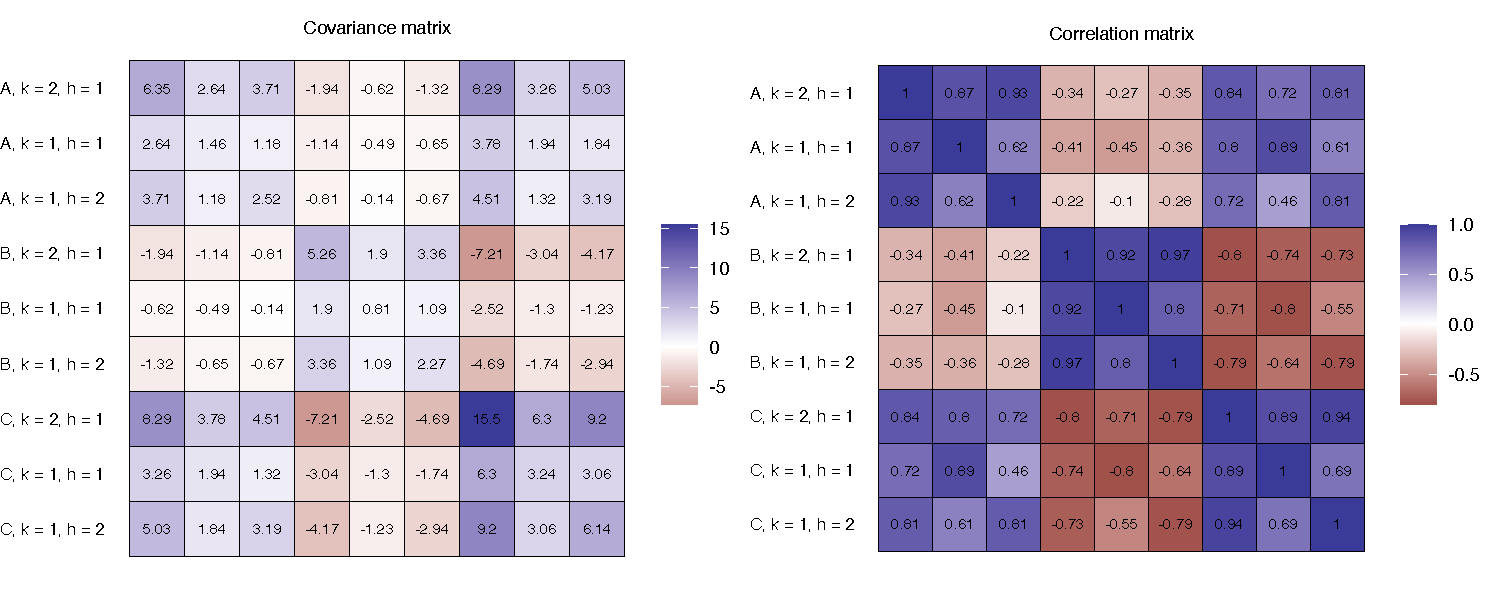
\includegraphics[width = \linewidth]{fig/AR/covcor.pdf}
	\caption{Simulation experiment. True cross-temporal covariance (left) and correlation (right) error matrix of the reconciled forecasts with $\sigma_B = 0.9$, $\sigma_C = 1.8$, $\phivet_B = [1.34\; -0.74]'$, $\phivet_C = [0.95\; -0.42]'$ and $\rho = -0.8$.}
	\label{fig:covcorMC}
\end{figure}

To construct cross-temporal samples of the base forecasts, we use the Gaussian and bootstrap approaches discussed in Sections 3.1 and 3.2, respectively. For the parametric approach we use multi-step residuals with the different covariance matrix structures analyzed in 4.1, while for the non-parametric approach, we use regular one-step residuals. We do not use overlapping residuals in our analysis as we have the advantage of generating a large number of observation. Ten different reconciliation approaches have been adopted (see Table 2): ct$(bu)$, ct$(shr_{cs}, bu_{te})$, ct$(wlsv_{te}, bu_{cs})$, oct$(wlsv)$, oct$(bdshr)$, oct$_h(shr)$, oct$_h(bshr)$, oct$_h(hshr)$ and oct$_h(hbshr)$.



\subsection{Covariance matrix comparison and forecast accuracy scores}\label{ssec:acc_scores}

To compare the true covariance matrix $\Omegavet_{ct}$ with the estimated covariance matrix $\widehat{\Omegavet}$, we use the Frobenius norm to quantify the difference between two matrices: 
$$\lVert \Dvet \rVert_F = \displaystyle\sqrt{\sum_{i = 1}^{n(k^\ast + m)}\sum_{j = 1}^{n(k^\ast + m)}|d_{i,j}|^2}$$ where $\Dvet = \widehat{\Omegavet} - \Omegavet_{ct}$. The true covariance matrix, shown in \autoref{fig:covcorMC}, was compared to the estimated covariance matrices obtained using various reconciliation approaches and techniques for generating sample paths of the base forecasts. Thus, we should be able to determine which reconciliation approach and simulation technique produce an accurate estimate of the covariance matrix. Other types of matrix norms were also considered with similar results.

From \autoref{tab:ar2norm}, it appears that the reconciled covariance matrices are always closer to the true matrix than the base forecast matrix when using both the Gaussian and the bootstrap  approach. Overall, there are no major differences in the findings when using either one-step or multi-step residuals in cross-temporal forecast reconciliation. In fact, using approaches like oct$(bdshr)$, we obtain results that are consistent with approaches such as oct$_h(shr)$, where no temporal and/or cross-sectional correlation assumptions are imposed. It is worth noting that the $HB$ covariance matrix when used to calculate the base forecasts samples, is not changed by the reconciliation step (see \autoref{app:shr}). In conclusion, our results suggest that using multi-step residuals or bootstrap techniques may help find a “good" estimate of the covariance matrix, which can be further improved by the reconciliation.

\begin{table}[!t]
	\centering
	\begingroup
	\spacingset{1}
	\fontsize{9}{11}\selectfont
	
\begin{tabular}[t]{l|>{}ccccc}
\toprule
\multicolumn{1}{c}{\textbf{}} & \multicolumn{5}{c}{\textbf{Generation of the base forecasts paths}} \\
\cmidrule(l{0pt}r{0pt}){2-6}
\multicolumn{1}{c}{\makecell[c]{\bfseries Reconciliation\\\bfseries approach}} & \multicolumn{1}{c}{ctjb} & \multicolumn{4}{c}{\makecell[c]{Gaussian approach\textsuperscript{*}}} \\
\multicolumn{1}{c}{} &  & G & B & H & HB\\
\midrule
base & \textcolor{black}{8.260} & \textcolor{black}{7.748} & \textcolor{black}{6.549} & \textcolor{black}{3.409} & \textcolor{black}{2.215}\\
ct$(bu)$ & \textcolor{black}{3.195} & \textcolor{black}{2.215} & \textcolor{black}{2.215} & \textcolor{black}{\textbf{2.215}} & \textcolor{black}{2.215}\\
ct$(shr_{cs}, bu_{te})$ & \textcolor{black}{3.202} & \textcolor{black}{2.224} & \textcolor{black}{2.215} & \textcolor{black}{2.224} & \textcolor{black}{2.215}\\
ct$(wlsv_{te}, bu_{cs})$ & \textcolor{black}{\textbf{3.183}} & \textcolor{black}{\textbf{2.188}} & \textcolor{black}{2.188} & \textcolor{black}{\textbf{2.215}} & \textcolor{black}{2.215}\\
oct$(wlsv)$ & \textcolor{black}{3.766} & \textcolor{black}{3.082} & \textcolor{black}{2.191} & \textcolor{black}{2.910} & \textcolor{black}{2.215}\\
oct$(bdshr)$ & \textcolor{black}{3.203} & \textcolor{black}{2.195} & \textcolor{blue}{\textbf{2.184}} & \textcolor{black}{2.224} & \textcolor{black}{\textbf{2.215}}\\
oct$_h(shr)$ & \textcolor{black}{3.251} & \textcolor{black}{2.260} & \textcolor{black}{2.202} & \textcolor{black}{2.226} & \textcolor{black}{2.215}\\
oct$_h(bshr)$ & \textcolor{black}{3.602} & \textcolor{black}{2.720} & \textcolor{black}{2.220} & \textcolor{black}{2.756} & \textcolor{black}{2.215}\\
oct$_h(hshr)$ & \textcolor{black}{4.869} & \textcolor{black}{4.138} & \textcolor{black}{4.167} & \textcolor{black}{2.225} & \textcolor{black}{2.215}\\
\bottomrule
\multicolumn{6}{l}{\rule{0pt}{1em}\rule{0pt}{1.75em}\makecell[l]{$^\ast$The Gaussian method employs a sample covariance\\ with multi-step residuals.}}\\
\end{tabular}

	\endgroup
	\caption{Simulation experiment. Frobenius norm between the true and the estimated covariance matrix for different reconciliation approaches and different techniques for simulating the base forecasts. Entries in bold represent the lowest value for each column, while the blue entry represent the global minimum. The reconciliation approaches are described in Table 2.}
	\label{tab:ar2norm}
\end{table}

A limitation of this simulation setting is that we are using a high number of residuals, which may result in undervaluing the benefit from using the parameterization form of the covariance matrix such as $HB$, $H$, or $B$ (see Section 4). Additionally, shrinkage techniques often yield very similar results when we use the corresponding matrix with $\lambda = 0$ (full covariance matrix). 

In Tables \ref{tab:ar2crps} and \ref{tab:ar2es} are reported the $\operatorname{\overline{RelCRPS}}$ and ES ratio indices introduced in Sections 5 where low values indicate better quality of the forecasts. The good performance of the ct$(bu)$ approach can be explained by a good quality of the base forecasts at the bottom level for $k=1$, and therefore it is difficult for the other approaches to correctly adjust them using the somewhat less good forecasts of the higher temporal and cross-sectional levels. This also explains the good performance of ct$(shr_{cs}, bu_{te})$, which by definition only takes into account the information provided by the most temporally disaggregated base forecasts.
Looking at the optimal cross-temporal reconciliation approaches, it does not seem to be any advantage in using multi-step residuals to calculate the covariance matrix in the reconciliation step.

\begin{table}[!t]
	\centering
	\begingroup
	\spacingset{1}
	\fontsize{9}{11}\selectfont
	
\begin{tabular}[t]{c|>{}cccc>{}c|ccccc}
\toprule
\multicolumn{1}{c}{\textbf{}} & \multicolumn{10}{c}{\textbf{Base forecasts' sample approach}} \\
\cmidrule(l{0pt}r{0pt}){2-11}
\multicolumn{1}{c}{\makecell[c]{\bfseries Reconciliation\\\bfseries approach}} & \multicolumn{1}{c}{ctjb} & \multicolumn{4}{c}{\makecell[c]{Gaussian approach\textsuperscript{*}}} & \multicolumn{1}{c}{ctjb} & \multicolumn{4}{c}{\makecell[c]{Gaussian approach\textsuperscript{*}}} \\
\multicolumn{1}{c}{} &  & G & B & H & \multicolumn{1}{c}{HB} &  & G & B & H & HB\\
\midrule
\addlinespace[0.3em]
\multicolumn{1}{c}{} & \multicolumn{5}{c}{\textbf{$\forall k \in \{12,6,4,3,2,1\}$}} & \multicolumn{5}{c}{\textbf{$k = 1$}}\\
base & \textcolor{black}{1.000} & \textcolor{black}{0.971} & \textcolor{black}{0.971} & \textcolor{black}{0.973} & \textcolor{black}{0.973} & \textcolor{black}{1.000} & \textcolor{black}{0.972} & \textcolor{black}{0.972} & \textcolor{black}{0.972} & \textcolor{black}{0.972}\\
ct$(bu)$ & \textcolor{red}{1.321} & \textcolor{red}{1.011} & \textcolor{red}{1.011} & \textcolor{red}{1.011} & \textcolor{red}{1.011} & \textcolor{red}{1.077} & \textcolor{black}{0.983} & \textcolor{black}{0.982} & \textcolor{black}{0.982} & \textcolor{black}{0.982}\\
ct$(shr_{cs}, bu_{te})$ & \textcolor{red}{1.057} & \textcolor{black}{0.974} & \textcolor{black}{0.969} & \textcolor{black}{0.974} & \textcolor{black}{0.969} & \textcolor{black}{0.976} & \textcolor{black}{0.963} & \textcolor{black}{0.962} & \textcolor{black}{0.963} & \textcolor{black}{0.962}\\
ct$(wls_{cs}, bu_{te})$ & \textcolor{red}{1.082} & \textcolor{black}{0.977} & \textcolor{black}{0.976} & \textcolor{black}{0.977} & \textcolor{black}{0.976} & \textcolor{black}{0.986} & \textcolor{black}{0.965} & \textcolor{black}{0.965} & \textcolor{black}{0.965} & \textcolor{black}{0.965}\\
oct$(wlsv)$ & \textcolor{black}{0.987} & \textcolor{black}{0.959} & \textcolor{black}{0.959} & \textcolor{black}{0.958} & \textcolor{black}{0.957} & \textcolor{black}{0.952} & \textcolor{black}{0.957} & \textcolor{black}{0.957} & \textcolor{black}{0.957} & \textcolor{black}{0.957}\\
oct$(bdshr)$ & \textcolor{black}{\textbf{0.975}} & \textcolor{black}{\textbf{0.956}} & \textcolor{black}{\textbf{0.953}} & \textcolor{black}{\textbf{0.952}} & \textcolor{blue}{\textbf{0.951}} & \textcolor{blue}{\textbf{0.949}} & \textcolor{black}{\textbf{0.955}} & \textcolor{black}{\textbf{0.953}} & \textcolor{black}{\textbf{0.954}} & \textcolor{black}{\textbf{0.954}}\\
\addlinespace[0.3em]
\multicolumn{1}{c}{} & \multicolumn{5}{c}{\textbf{$k = 2$}} & \multicolumn{5}{c}{\textbf{$k = 3$}}\\
base & \textcolor{black}{1.000} & \textcolor{black}{0.970} & \textcolor{black}{0.969} & \textcolor{black}{0.970} & \textcolor{black}{0.971} & \textcolor{black}{1.000} & \textcolor{black}{0.971} & \textcolor{black}{0.971} & \textcolor{black}{0.972} & \textcolor{black}{0.973}\\
ct$(bu)$ & \textcolor{red}{1.189} & \textcolor{black}{0.999} & \textcolor{black}{0.999} & \textcolor{black}{0.999} & \textcolor{black}{0.999} & \textcolor{red}{1.273} & \textcolor{red}{1.010} & \textcolor{red}{1.010} & \textcolor{red}{1.010} & \textcolor{red}{1.010}\\
ct$(shr_{cs}, bu_{te})$ & \textcolor{red}{1.015} & \textcolor{black}{0.972} & \textcolor{black}{0.970} & \textcolor{black}{0.972} & \textcolor{black}{0.970} & \textcolor{red}{1.041} & \textcolor{black}{0.977} & \textcolor{black}{0.974} & \textcolor{black}{0.977} & \textcolor{black}{0.974}\\
ct$(wls_{cs}, bu_{te})$ & \textcolor{red}{1.031} & \textcolor{black}{0.975} & \textcolor{black}{0.974} & \textcolor{black}{0.975} & \textcolor{black}{0.974} & \textcolor{red}{1.062} & \textcolor{black}{0.980} & \textcolor{black}{0.979} & \textcolor{black}{0.980} & \textcolor{black}{0.979}\\
oct$(wlsv)$ & \textcolor{black}{0.972} & \textcolor{black}{0.961} & \textcolor{black}{0.960} & \textcolor{black}{0.960} & \textcolor{black}{0.960} & \textcolor{black}{0.983} & \textcolor{black}{0.963} & \textcolor{black}{0.962} & \textcolor{black}{0.962} & \textcolor{black}{0.962}\\
oct$(bdshr)$ & \textcolor{black}{\textbf{0.964}} & \textcolor{black}{\textbf{0.958}} & \textcolor{black}{\textbf{0.957}} & \textcolor{black}{\textbf{0.956}} & \textcolor{blue}{\textbf{0.956}} & \textcolor{black}{\textbf{0.972}} & \textcolor{black}{\textbf{0.960}} & \textcolor{black}{\textbf{0.958}} & \textcolor{black}{\textbf{0.957}} & \textcolor{blue}{\textbf{0.957}}\\
\addlinespace[0.3em]
\multicolumn{1}{c}{} & \multicolumn{5}{c}{\textbf{$k = 4$}} & \multicolumn{5}{c}{\textbf{$k = 6$}}\\
base & \textcolor{black}{1.000} & \textcolor{black}{0.973} & \textcolor{black}{0.973} & \textcolor{black}{0.974} & \textcolor{black}{0.975} & \textcolor{black}{1.000} & \textcolor{black}{0.976} & \textcolor{black}{0.976} & \textcolor{black}{0.978} & \textcolor{black}{0.978}\\
ct$(bu)$ & \textcolor{red}{1.340} & \textcolor{red}{1.016} & \textcolor{red}{1.015} & \textcolor{red}{1.015} & \textcolor{red}{1.015} & \textcolor{red}{1.450} & \textcolor{red}{1.023} & \textcolor{red}{1.023} & \textcolor{red}{1.023} & \textcolor{red}{1.023}\\
ct$(shr_{cs}, bu_{te})$ & \textcolor{red}{1.061} & \textcolor{black}{0.978} & \textcolor{black}{0.973} & \textcolor{black}{0.978} & \textcolor{black}{0.973} & \textcolor{red}{1.094} & \textcolor{black}{0.978} & \textcolor{black}{0.972} & \textcolor{black}{0.978} & \textcolor{black}{0.972}\\
ct$(wls_{cs}, bu_{te})$ & \textcolor{red}{1.087} & \textcolor{black}{0.982} & \textcolor{black}{0.980} & \textcolor{black}{0.982} & \textcolor{black}{0.980} & \textcolor{red}{1.127} & \textcolor{black}{0.982} & \textcolor{black}{0.981} & \textcolor{black}{0.982} & \textcolor{black}{0.981}\\
oct$(wlsv)$ & \textcolor{black}{0.990} & \textcolor{black}{0.962} & \textcolor{black}{0.961} & \textcolor{black}{0.961} & \textcolor{black}{0.960} & \textcolor{red}{1.001} & \textcolor{black}{0.960} & \textcolor{black}{0.959} & \textcolor{black}{0.958} & \textcolor{black}{0.957}\\
oct$(bdshr)$ & \textcolor{black}{\textbf{0.977}} & \textcolor{black}{\textbf{0.959}} & \textcolor{black}{\textbf{0.956}} & \textcolor{black}{\textbf{0.955}} & \textcolor{blue}{\textbf{0.954}} & \textcolor{black}{\textbf{0.985}} & \textcolor{black}{\textbf{0.956}} & \textcolor{black}{\textbf{0.953}} & \textcolor{black}{\textbf{0.950}} & \textcolor{blue}{\textbf{0.948}}\\
\addlinespace[0.3em]
\multicolumn{1}{c}{} & \multicolumn{5}{c}{\textbf{$k = 12$}} & \multicolumn{5}{c}{}\\
base & \textcolor{black}{\textbf{1.000}} & \textcolor{black}{0.968} & \textcolor{black}{0.967} & \textcolor{black}{0.969} & \textcolor{black}{0.969} &  &  &  &  & \\
ct$(bu)$ & \textcolor{red}{1.675} & \textcolor{red}{1.038} & \textcolor{red}{1.037} & \textcolor{red}{1.037} & \textcolor{red}{1.038} &  &  &  &  & \\
ct$(shr_{cs}, bu_{te})$ & \textcolor{red}{1.163} & \textcolor{black}{0.977} & \textcolor{black}{0.965} & \textcolor{black}{0.977} & \textcolor{black}{0.965} &  &  &  &  & \\
ct$(wls_{cs}, bu_{te})$ & \textcolor{red}{1.212} & \textcolor{black}{0.980} & \textcolor{black}{0.976} & \textcolor{black}{0.980} & \textcolor{black}{0.976} &  &  &  &  & \\
oct$(wlsv)$ & \textcolor{red}{1.025} & \textcolor{black}{0.954} & \textcolor{black}{0.953} & \textcolor{black}{0.949} & \textcolor{black}{0.947} &  &  &  &  & \\
oct$(bdshr)$ & \textcolor{red}{1.002} & \textcolor{black}{\textbf{0.950}} & \textcolor{black}{\textbf{0.944}} & \textcolor{black}{\textbf{0.939}} & \textcolor{blue}{\textbf{0.935}} &  &  &  &  & \\
\bottomrule
\multicolumn{11}{l}{\rule{0pt}{1em}\rule{0pt}{2em}\textsuperscript{*}\makecell[l]{The Gaussian method employs a sample covariance matrix and includes four techniques (G, B, H, HB)\\ with multi-step residuals.}}\\
\end{tabular}

	\endgroup
	\caption{Simulation experiment. $\overline{RelCRPS}$ defined in Section 5. Approaches performing worse than the benchmark (bootstrap base forecasts, ctjb) are highlighted in red, the best for each column is marked in bold, and the overall lowest value is highlighted in blue. The reconciliation approaches are described in Table 2.}
	\label{tab:ar2crps}
\end{table}

\begin{table}[!t]
	\centering
	\begingroup
	\spacingset{1}
	\fontsize{9}{11}\selectfont
	
\begin{tabular}[t]{c|>{}cccc>{}c|ccccc}
\toprule
\multicolumn{1}{c}{\textbf{}} & \multicolumn{10}{c}{\textbf{Base forecasts' sample approach}} \\
\cmidrule(l{0pt}r{0pt}){2-11}
\multicolumn{1}{c}{\makecell[c]{\bfseries Reconciliation\\\bfseries approach}} & \multicolumn{1}{c}{ctjb} & \multicolumn{4}{c}{\makecell[c]{Gaussian approach\textsuperscript{*}}} & \multicolumn{1}{c}{ctjb} & \multicolumn{4}{c}{\makecell[c]{Gaussian approach\textsuperscript{*}}} \\
\multicolumn{1}{c}{} &  & G$_{h}$ & H$_{h}$ & G$_{oh}$ & \multicolumn{1}{c}{H$_{oh}$} &  & G$_{h}$ & H$_{h}$ & G$_{oh}$ & \multicolumn{1}{c}{H$_{oh}$}\\
\midrule
\addlinespace[0.3em]
\multicolumn{1}{c}{} & \multicolumn{5}{c}{\textbf{$\forall k \in \{4,2,1\}$}} & \multicolumn{5}{c}{\textbf{$k = 1$}}\\
base & \textcolor{black}{1.000} & \textcolor{black}{0.970} & \textcolor{black}{0.988} & \textcolor{black}{0.960} & \textcolor{black}{0.970} & \textcolor{black}{1.000} & \textcolor{black}{0.977} & \textcolor{black}{0.977} & \textcolor{black}{0.965} & \textcolor{black}{0.965}\\
ct$(shr_{cs}, bu_{te})$ & \textcolor{black}{0.897} & \textcolor{black}{0.944} & \textcolor{black}{0.944} & \textcolor{black}{0.973} & \textcolor{black}{0.973} & \textcolor{black}{0.964} & \textcolor{red}{1.001} & \textcolor{red}{1.001} & \textcolor{red}{1.033} & \textcolor{red}{1.033}\\
ct$(wls_{cs}, bu_{te})$ & \textcolor{black}{\textbf{0.886}} & \textcolor{black}{0.880} & \textcolor{black}{\textbf{0.880}} & \textcolor{blue}{\textbf{0.860}} & \textcolor{black}{\textbf{0.860}} & \textcolor{black}{\textbf{0.954}} & \textcolor{black}{\textbf{0.944}} & \textcolor{black}{\textbf{0.945}} & \textcolor{blue}{\textbf{0.928}} & \textcolor{black}{\textbf{0.928}}\\
oct$_o(wlsv)$ & \textcolor{black}{0.891} & \textcolor{black}{\textbf{0.879}} & \textcolor{black}{0.881} & \textcolor{black}{0.864} & \textcolor{black}{0.864} & \textcolor{black}{0.958} & \textcolor{black}{0.945} & \textcolor{black}{0.945} & \textcolor{black}{0.931} & \textcolor{black}{0.931}\\
oct$_o(bdshr)$ & \textcolor{black}{0.940} & \textcolor{black}{0.928} & \textcolor{black}{0.910} & \textcolor{black}{0.918} & \textcolor{black}{0.895} & \textcolor{red}{1.004} & \textcolor{black}{0.986} & \textcolor{black}{0.971} & \textcolor{black}{0.980} & \textcolor{black}{0.961}\\
oct$_{oh}(shr)$ & \textcolor{red}{1.059} & \textcolor{red}{1.015} & \textcolor{black}{0.956} & \textcolor{red}{1.053} & \textcolor{black}{0.945} & \textcolor{red}{1.130} & \textcolor{red}{1.063} & \textcolor{red}{1.019} & \textcolor{red}{1.121} & \textcolor{red}{1.016}\\
oct$_{oh}(hshr)$ & \textcolor{black}{0.986} & \textcolor{black}{0.968} & \textcolor{black}{0.999} & \textcolor{black}{0.959} & \textcolor{black}{0.992} & \textcolor{red}{1.053} & \textcolor{red}{1.034} & \textcolor{red}{1.049} & \textcolor{red}{1.024} & \textcolor{red}{1.055}\\
\addlinespace[0.3em]
\multicolumn{1}{c}{} & \multicolumn{5}{c}{\textbf{$k = 2$}} & \multicolumn{5}{c}{\textbf{$k = 4$}}\\
base & \textcolor{black}{1.000} & \textcolor{black}{0.972} & \textcolor{black}{0.985} & \textcolor{black}{0.959} & \textcolor{black}{0.969} & \textcolor{black}{1.000} & \textcolor{black}{0.959} & \textcolor{red}{1.000} & \textcolor{black}{0.957} & \textcolor{black}{0.976}\\
ct$(shr_{cs}, bu_{te})$ & \textcolor{black}{0.915} & \textcolor{black}{0.961} & \textcolor{black}{0.960} & \textcolor{black}{0.991} & \textcolor{black}{0.991} & \textcolor{black}{0.818} & \textcolor{black}{0.874} & \textcolor{black}{0.874} & \textcolor{black}{0.899} & \textcolor{black}{0.900}\\
ct$(wls_{cs}, bu_{te})$ & \textcolor{black}{\textbf{0.904}} & \textcolor{black}{0.896} & \textcolor{black}{\textbf{0.896}} & \textcolor{blue}{\textbf{0.877}} & \textcolor{black}{\textbf{0.877}} & \textcolor{black}{\textbf{0.807}} & \textcolor{black}{0.805} & \textcolor{black}{\textbf{0.805}} & \textcolor{blue}{\textbf{0.782}} & \textcolor{black}{\textbf{0.783}}\\
oct$_o(wlsv)$ & \textcolor{black}{0.908} & \textcolor{black}{\textbf{0.895}} & \textcolor{black}{0.898} & \textcolor{black}{0.881} & \textcolor{black}{0.882} & \textcolor{black}{0.812} & \textcolor{black}{\textbf{0.802}} & \textcolor{black}{0.806} & \textcolor{black}{0.786} & \textcolor{black}{0.786}\\
oct$_o(bdshr)$ & \textcolor{black}{0.960} & \textcolor{black}{0.947} & \textcolor{black}{0.929} & \textcolor{black}{0.938} & \textcolor{black}{0.915} & \textcolor{black}{0.860} & \textcolor{black}{0.856} & \textcolor{black}{0.836} & \textcolor{black}{0.841} & \textcolor{black}{0.816}\\
oct$_{oh}(shr)$ & \textcolor{red}{1.082} & \textcolor{red}{1.029} & \textcolor{black}{0.973} & \textcolor{red}{1.076} & \textcolor{black}{0.963} & \textcolor{black}{0.971} & \textcolor{black}{0.954} & \textcolor{black}{0.882} & \textcolor{black}{0.967} & \textcolor{black}{0.861}\\
oct$_{oh}(hshr)$ & \textcolor{red}{1.007} & \textcolor{black}{0.988} & \textcolor{red}{1.017} & \textcolor{black}{0.979} & \textcolor{red}{1.014} & \textcolor{black}{0.904} & \textcolor{black}{0.888} & \textcolor{black}{0.934} & \textcolor{black}{0.881} & \textcolor{black}{0.913}\\
\bottomrule
\multicolumn{11}{l}{\rule{0pt}{1em}\rule{0pt}{1.75em}\makecell[l]{$^\ast$The Gaussian method employs a sample covariance matrix:\\G$_{h}$ and H$_{h}$ use multi-step residuals and G$_{oh}$ and H$_{oh}$ use overlapping and multi-step residuals.}}\\
\end{tabular}

	\endgroup
	\caption{Simulation experiment. ES ratio indices defined in Section 5. Approaches performing worse than the benchmark (bootstrap base forecasts, ctjb) are highlighted in red, the best for each column is marked in bold, and the overall lowest value is highlighted in blue. The reconciliation approaches are described in Table 2.}
	\label{tab:ar2es}
\end{table}

In conclusion, we found that simulating base forecasts from multi-step residuals allows us to estimate a covariance matrix close to the true one. Additionally, we observed that reconciliation could be used to further improve the accuracy of these estimates: accurate base forecasts for $k=1$ assist the good performance for bottom-up and optimal cross-temporal reconciliation approaches, such as oct$(wlsv)$ and oct$(bdshr)$, which perform well in terms of both CRPS and ES.


%\newpage
\subsection{Cross-temporal covariance matrix}\label{app:ar2}

We assume two AR(2) processes with correlated errors such that
$$
	y_{i,t} = \phi_{i,1}y_{i,t-1} + \phi_{i,2}y_{i,t-2} + \varepsilon_{i,t}
$$
where $\epsvet_t \sim \mathcal{N}_{2}\left(\Zerovet_{(2\times 1)}, \Omegavet_{cs}\right)$ and $i \in \{B, C\}$. Let $y_{i,T+h}$ be the true observation for the $i^{th}$ series and $\widetilde{y}_{i,T+h}$ the corresponding forecasts such that
$$
	\begin{array}{rl}
		y_{i,T+1} & = \phi_{i,1}y_{i,T} + \phi_{i,2}y_{i,T-1} + \varepsilon_{i,T+1} \\
		y_{i,T+2} & = \phi_{i,1}y_{i,T+1} + \phi_{i,2}y_{i,T} + \varepsilon_{i,T+2}
	\end{array}
	\quad\text{and}\quad
	\begin{array}{rl}
		\widetilde{y}_{i,T+1} & = \phi_{i,1}y_{i,T} + \phi_{i,2}y_{i,T-1}             \\
		\widetilde{y}_{i,T+2} & = \phi_{i,1}\widetilde{y}_{i,T+1} + \phi_{i,2}y_{i,T}
	\end{array}\;,
$$
then
\begin{align*}
	y_{i,T+1} - \widetilde{y}_{i,T+1} & = \varepsilon_{i,T+1}                                   \\
	y_{i,T+2} - \widetilde{y}_{i,T+2} & = \varepsilon_{i,T+2} + \phi_{i,1} \varepsilon_{i,T+1}.
\end{align*}
Finally, we can compute each element of the high frequency bottom time series covariance matrix
\begin{align*}\allowdisplaybreaks[2]
	Var\left(y_{i,T+1}-\widetilde{y}_{i,T+1}\right) & = \sigma_i^2, \quad \forall i \in \{B, C\}                                                                    \\
	Var\left(y_{i,T+2}-\widetilde{y}_{i,T+2}\right) & = \sigma_i^2\left(1+\phi_{i,1}^2\right), \quad \forall i \in \{B, C\}\\
	Cov\left[\left(y_{i,T+2}-\widetilde{y}_{i,T+2}\right), \left(y_{i,T+1}-\widetilde{y}_{i,T+1}\right)\right] & = 	Cov\left[\left(y_{i,T+1}-\widetilde{y}_{i,T+1}\right), \left(y_{i,T+2}-\widetilde{y}_{i,T+2}\right)\right] \\
		& = \phi_{i, 1}\sigma_{i}^2, \quad \forall i \in \{B, C\} \\
	Cov\left[\left(y_{i,T+1}-\widetilde{y}_{i,T+1}\right), \left(y_{j,T+1}-\widetilde{y}_{j,T+1}\right)\right] & = 	Cov\left[\left(y_{j,T+1}-\widetilde{y}_{j,T+1}\right), \left(y_{i,T+1}-\widetilde{y}_{i,T+1}\right)\right] \\
	& = \sigma_{i, j}, \quad \forall i,j \in \{B, C\}, \quad i\neq j\\
	Cov\left[\left(y_{i,T+2}-\widetilde{y}_{i,T+2}\right), \left(y_{j,T+1}-\widetilde{y}_{j,T+1}\right)\right] & = 	Cov\left[\left(y_{j,T+1}-\widetilde{y}_{j,T+1}\right), \left(y_{i,T+2}-\widetilde{y}_{i,T+2}\right)\right] \\
	& = \phi_{i,1}\sigma_{i, j}, \quad \forall i,j \in \{B, C\}, \quad i\neq j                                      \\
	Cov\left[\left(y_{i,T+2}-\widetilde{y}_{i,T+2}\right), \left(y_{j,T+2}-\widetilde{y}_{j,T+2}\right)\right] & = 	Cov\left[\left(y_{j,T+2}-\widetilde{y}_{j,T+2}\right), \left(y_{i,T+2}-\widetilde{y}_{i,T+2}\right)\right] \\
	& = \sigma_{i, j}\left(1+\phi_{i,1}\phi_{j,1}\right), \quad \forall i,j \in \{B, C\}, \quad i\neq j.
\end{align*}
In conclusion,
$$
	\Omegavet_{\textit{hf-bts}} = \begin{bmatrix}
		\sigma^2_B & & & \\
		\phi_{B,1}\sigma_B^2  & \sigma_B^2\left(1+\phi_{B,1}^2\right) & & \\
		\sigma_{BC} & \phi_{B,1}\sigma_{BC} & \sigma_C^2 & \\
		\phi_{C,1}\sigma_{BC} & \sigma_{BC}\left(1+\phi_{B,1}\phi_{C,1} \right) & \phi_{C,1}\sigma_C^2 & \sigma_C^2\left(1+\phi_{C,1}^2\right) \\
	\end{bmatrix}
$$
and
$$
	\Omegavet_{ct} = \Svet_{ct}\Omegavet_{\textit{hf-bts}}\Svet_{ct}'.
$$

%\newpage
\subsection{One-step residuals and shrinkage covariance matrix}

In Section 4.1, we discussed the use of one-step residuals in estimating the covariance matrix. In particular we point out that one-step residuals lead to a biased estimate of the covariance matrix where some correlation are zeros by definition (see \autoref{fig:ar2covcor_app}). 
In addition, Tables \ref{tab:ar2norm_app}, \ref{tab:ar2crps_app} and \ref{tab:ar2es_app} show the Frobenius norm, CRPS, and ES skill scores as explained in the paper to investigate the effectiveness of one-step residuals. 
Moreover, in Tables \ref{tab:ar2crps_app_shr} and \ref{tab:ar2es_app_shr}, we have utilized a shrinkage matrix rather than the sample covariance matrix to assess the performance of our approach.

\begin{figure}[p]
	\centering
	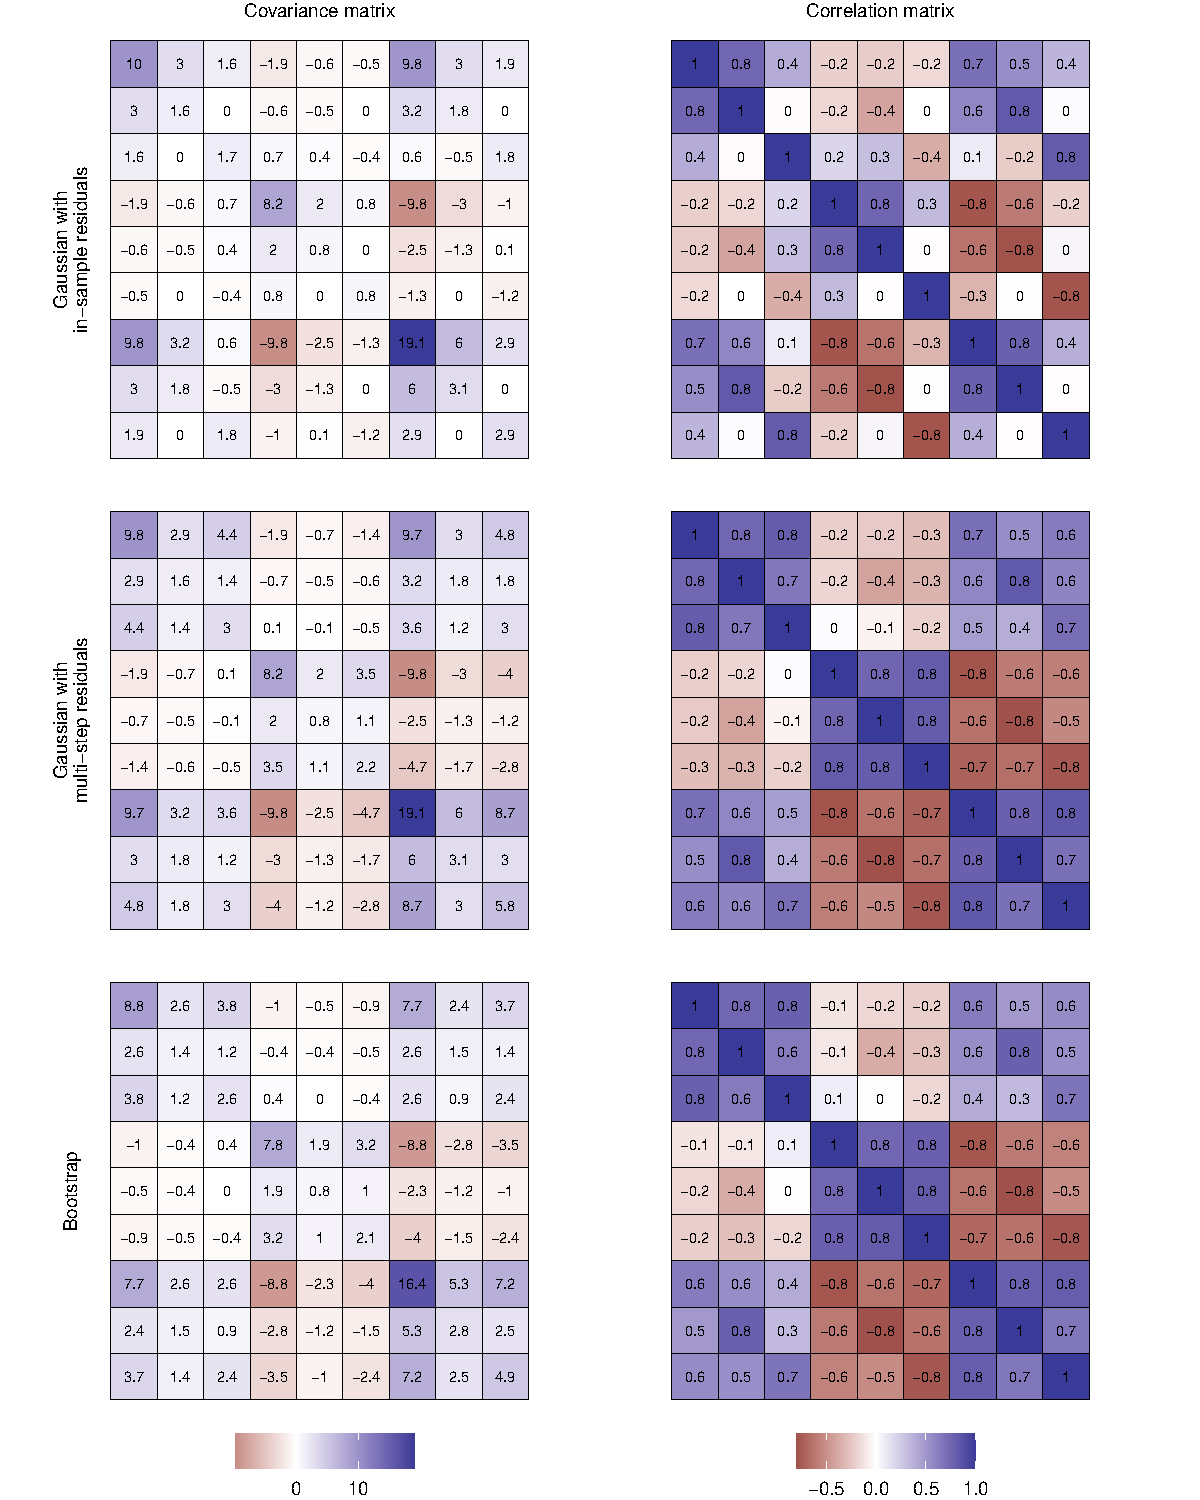
\includegraphics[width = \linewidth]{fig/AR/base_cov_app.pdf}
	\caption{Comparison of estimated covariance and correlation matrices (first simulation) for base forecasts using a parametric Gaussian (with one-step residuals) approach. The true covariance and correlation matrices are shown in Figure 7.}
	\label{fig:ar2covcor_app}
\end{figure}

\begin{table}[H]
	\centering
	\begingroup
	\spacingset{1}
	\fontsize{9}{11}\selectfont
	
\begin{tabular}[t]{>{\centering\arraybackslash}m{2.5cm}ccccccccc}
\toprule
\multicolumn{1}{c}{\textbf{}} & \multicolumn{9}{c}{\textbf{Base forecasts' sample approach}} \\
\cmidrule(l{0pt}r{0pt}){2-10}
\multicolumn{1}{c}{} & \multicolumn{1}{c}{} & \multicolumn{8}{c}{\makecell[c]{Gaussian approach: sample covariance matrix}} \\
\multicolumn{1}{c}{\makecell[c]{\bfseries Reconciliation\\\bfseries approach}} & \multicolumn{1}{c}{ctjb} & \multicolumn{4}{c}{In-sample residuals} & \multicolumn{4}{c}{Multi-step residuals} \\
 &  & G & B & H & HB & G & B & H & HB\\
\midrule
base & \textcolor{black}{8.260} & \textcolor{black}{17.638} & \textcolor{black}{16.733} & \textcolor{black}{22.178} & \textcolor{black}{21.789} & \textcolor{black}{7.748} & \textcolor{black}{6.549} & \textcolor{black}{3.409} & \textcolor{black}{2.215}\\
ct$(bu)$ & \textcolor{black}{3.195} & \textcolor{black}{21.789} & \textcolor{black}{21.789} & \textcolor{black}{\textbf{21.789}} & \textcolor{black}{21.789} & \textcolor{black}{2.215} & \textcolor{black}{2.215} & \textcolor{black}{\textbf{2.215}} & \textcolor{black}{2.215}\\
ct$(shr_{cs}, bu_{te})$ & \textcolor{black}{3.202} & \textcolor{black}{21.942} & \textcolor{black}{21.789} & \textcolor{black}{21.942} & \textcolor{black}{21.789} & \textcolor{black}{2.224} & \textcolor{black}{2.215} & \textcolor{black}{2.224} & \textcolor{black}{2.215}\\
ct$(wlsv_{te}, bu_{cs})$ & \textcolor{black}{\textbf{3.183}} & \textcolor{black}{18.237} & \textcolor{black}{18.237} & \textcolor{black}{21.789} & \textcolor{black}{21.789} & \textcolor{black}{\textbf{2.188}} & \textcolor{black}{2.188} & \textcolor{black}{\textbf{2.215}} & \textcolor{black}{2.215}\\
oct$(wlsv)$ & \textcolor{black}{3.766} & \textcolor{black}{19.174} & \textcolor{black}{18.611} & \textcolor{black}{22.304} & \textcolor{black}{21.789} & \textcolor{black}{3.082} & \textcolor{black}{2.191} & \textcolor{black}{2.910} & \textcolor{black}{2.215}\\
oct$(bdshr)$ & \textcolor{black}{3.203} & \textcolor{black}{18.559} & \textcolor{black}{18.416} & \textcolor{black}{21.937} & \textcolor{black}{21.789} & \textcolor{black}{2.195} & \textcolor{blue}{\textbf{2.184}} & \textcolor{black}{2.224} & \textcolor{black}{\textbf{2.215}}\\
oct$(shr)$ & \textcolor{black}{5.217} & \textcolor{black}{25.015} & \textcolor{black}{23.457} & \textcolor{black}{23.413} & \textcolor{black}{\textbf{21.789}} & \textcolor{black}{2.260} & \textcolor{black}{2.202} & \textcolor{black}{2.226} & \textcolor{black}{2.215}\\
oct$(bshr)$ & \textcolor{black}{5.282} & \textcolor{black}{23.772} & \textcolor{black}{23.997} & \textcolor{black}{22.146} & \textcolor{black}{21.789} & \textcolor{black}{2.720} & \textcolor{black}{2.220} & \textcolor{black}{2.756} & \textcolor{black}{2.215}\\
oct$(hshr)$ & \textcolor{black}{6.161} & \textcolor{black}{\textbf{11.336}} & \textcolor{black}{\textbf{10.940}} & \textcolor{black}{23.598} & \textcolor{black}{\textbf{21.789}} & \textcolor{black}{4.138} & \textcolor{black}{4.167} & \textcolor{black}{2.225} & \textcolor{black}{2.215}\\
oct$(hbshr)$ & \textcolor{black}{5.731} & \textcolor{black}{11.379} & \textcolor{black}{10.940} & \textcolor{black}{22.146} & \textcolor{black}{21.789} & \textcolor{black}{5.085} & \textcolor{black}{4.167} & \textcolor{black}{2.756} & \textcolor{black}{2.215}\\
oct$_h(shr)$ & \textcolor{black}{3.251} & \textcolor{black}{20.965} & \textcolor{black}{19.992} & \textcolor{black}{22.079} & \textcolor{black}{\textbf{21.789}} & \textcolor{black}{2.260} & \textcolor{black}{2.202} & \textcolor{black}{2.226} & \textcolor{black}{2.215}\\
oct$_h(bshr)$ & \textcolor{black}{3.602} & \textcolor{black}{21.306} & \textcolor{black}{21.022} & \textcolor{black}{22.146} & \textcolor{black}{21.789} & \textcolor{black}{2.720} & \textcolor{black}{2.220} & \textcolor{black}{2.756} & \textcolor{black}{2.215}\\
oct$_h(hshr)$ & \textcolor{black}{4.869} & \textcolor{black}{11.405} & \textcolor{black}{10.940} & \textcolor{black}{22.037} & \textcolor{black}{21.789} & \textcolor{black}{4.138} & \textcolor{black}{4.167} & \textcolor{black}{2.225} & \textcolor{black}{2.215}\\
oct$_h(hbshr)$ & \textcolor{black}{5.731} & \textcolor{black}{11.379} & \textcolor{black}{10.940} & \textcolor{black}{22.146} & \textcolor{black}{21.789} & \textcolor{black}{5.085} & \textcolor{black}{4.167} & \textcolor{black}{2.756} & \textcolor{black}{2.215}\\
\bottomrule
\end{tabular}

	\endgroup
	\caption{Frobenius norm between the true and the estimated covariance matrix for different reconciliation approaches and different techniques for simulating the base forecasts. Entries in bold represent the lowest value for each column, while the blue entry represent the global minimum. The reconciliation approaches are described in Table 2.}
	\label{tab:ar2norm_app}
\end{table}

\begin{table}[H]
	\centering
	\begingroup
	\spacingset{1}
	\fontsize{9}{11}\selectfont
	
\begin{tabular}[t]{l|ccccccccc}
\toprule
\multicolumn{1}{c}{\textbf{}} & \multicolumn{9}{c}{\textbf{Generation of the base forecasts paths}} \\
\cmidrule(l{0pt}r{0pt}){2-10}
\multicolumn{1}{c}{} & \multicolumn{1}{c}{} & \multicolumn{8}{c}{\makecell[c]{Gaussian approach: sample covariance matrix}} \\
\multicolumn{1}{c}{\makecell[c]{\bfseries Reconciliation\\\bfseries approach}} & \multicolumn{1}{c}{ctjb} & \multicolumn{4}{c}{In-sample residuals} & \multicolumn{4}{c}{Multi-step residuals} \\
 &  & G & B & H & HB & G & B & H & HB\\
\midrule
\addlinespace[0.3em]
\multicolumn{10}{c}{\textbf{$\forall k \in \{2,1\}$}}\\
base & \textcolor{black}{1.000} & \textcolor{red}{1.008} & \textcolor{red}{1.009} & \textcolor{red}{1.044} & \textcolor{red}{1.047} & \textcolor{black}{0.998} & \textcolor{black}{0.999} & \textcolor{red}{1.002} & \textcolor{red}{1.004}\\
ct$(bu)$ & \textcolor{black}{0.901} & \textcolor{black}{0.930} & \textcolor{black}{0.929} & \textcolor{black}{0.929} & \textcolor{black}{0.929} & \textcolor{black}{0.900} & \textcolor{black}{0.900} & \textcolor{black}{0.900} & \textcolor{black}{0.900}\\
ct$(shr_{cs}, bu_{te})$ & \textcolor{black}{\textbf{0.901}} & \textcolor{black}{\textbf{0.929}} & \textcolor{black}{0.928} & \textcolor{black}{\textbf{0.929}} & \textcolor{black}{\textbf{0.928}} & \textcolor{black}{\textbf{0.900}} & \textcolor{blue}{\textbf{0.899}} & \textcolor{black}{\textbf{0.900}} & \textcolor{black}{\textbf{0.900}}\\
ct$(wlsv_{te}, bu_{cs})$ & \textcolor{black}{0.910} & \textcolor{black}{0.930} & \textcolor{black}{0.929} & \textcolor{black}{0.939} & \textcolor{black}{0.939} & \textcolor{black}{0.916} & \textcolor{black}{0.916} & \textcolor{black}{0.916} & \textcolor{black}{0.917}\\
oct$(wlsv)$ & \textcolor{black}{0.922} & \textcolor{black}{0.942} & \textcolor{black}{0.944} & \textcolor{black}{0.951} & \textcolor{black}{0.953} & \textcolor{black}{0.930} & \textcolor{black}{0.930} & \textcolor{black}{0.930} & \textcolor{black}{0.931}\\
oct$(bdshr)$ & \textcolor{black}{0.910} & \textcolor{black}{0.930} & \textcolor{black}{0.930} & \textcolor{black}{0.939} & \textcolor{black}{0.938} & \textcolor{black}{0.916} & \textcolor{black}{0.915} & \textcolor{black}{0.916} & \textcolor{black}{0.916}\\
oct$(shr)$ & \textcolor{black}{0.941} & \textcolor{black}{0.999} & \textcolor{black}{0.985} & \textcolor{black}{0.983} & \textcolor{black}{0.973} & \textcolor{black}{0.903} & \textcolor{black}{0.902} & \textcolor{black}{0.902} & \textcolor{black}{0.903}\\
oct$(bshr)$ & \textcolor{black}{0.951} & \textcolor{black}{0.995} & \textcolor{red}{1.000} & \textcolor{black}{0.983} & \textcolor{black}{0.986} & \textcolor{black}{0.922} & \textcolor{black}{0.922} & \textcolor{black}{0.921} & \textcolor{black}{0.922}\\
oct$(hshr)$ & \textcolor{black}{0.987} & \textcolor{black}{0.995} & \textcolor{black}{0.993} & \textcolor{red}{1.039} & \textcolor{red}{1.026} & \textcolor{black}{0.972} & \textcolor{black}{0.972} & \textcolor{black}{0.974} & \textcolor{black}{0.975}\\
oct$(hbshr)$ & \textcolor{black}{0.987} & \textcolor{black}{0.995} & \textcolor{black}{0.996} & \textcolor{red}{1.024} & \textcolor{red}{1.028} & \textcolor{black}{0.985} & \textcolor{black}{0.985} & \textcolor{black}{0.987} & \textcolor{black}{0.989}\\
oct$_h(shr)$ & \textcolor{black}{0.904} & \textcolor{black}{0.929} & \textcolor{black}{\textbf{0.928}} & \textcolor{black}{0.932} & \textcolor{black}{0.932} & \textcolor{black}{0.903} & \textcolor{black}{0.902} & \textcolor{black}{0.902} & \textcolor{black}{0.903}\\
oct$_h(bshr)$ & \textcolor{black}{0.923} & \textcolor{black}{0.948} & \textcolor{black}{0.952} & \textcolor{black}{0.951} & \textcolor{black}{0.954} & \textcolor{black}{0.922} & \textcolor{black}{0.922} & \textcolor{black}{0.921} & \textcolor{black}{0.922}\\
oct$_h(hshr)$ & \textcolor{black}{0.974} & \textcolor{black}{0.982} & \textcolor{black}{0.982} & \textcolor{red}{1.012} & \textcolor{red}{1.012} & \textcolor{black}{0.972} & \textcolor{black}{0.972} & \textcolor{black}{0.974} & \textcolor{black}{0.975}\\
oct$_h(hbshr)$ & \textcolor{black}{0.987} & \textcolor{black}{0.995} & \textcolor{black}{0.996} & \textcolor{red}{1.024} & \textcolor{red}{1.028} & \textcolor{black}{0.985} & \textcolor{black}{0.985} & \textcolor{black}{0.987} & \textcolor{black}{0.989}\\
\addlinespace[0.3em]
\multicolumn{10}{c}{\textbf{$k = 1$}}\\
base & \textcolor{black}{1.000} & \textcolor{red}{1.017} & \textcolor{red}{1.019} & \textcolor{red}{1.017} & \textcolor{red}{1.019} & \textcolor{black}{0.998} & \textcolor{black}{0.999} & \textcolor{black}{0.999} & \textcolor{black}{1.000}\\
ct$(bu)$ & \textcolor{black}{0.978} & \textcolor{black}{0.994} & \textcolor{black}{0.994} & \textcolor{black}{0.994} & \textcolor{black}{0.994} & \textcolor{black}{0.976} & \textcolor{black}{0.976} & \textcolor{black}{0.977} & \textcolor{black}{0.977}\\
ct$(shr_{cs}, bu_{te})$ & \textcolor{black}{\textbf{0.977}} & \textcolor{black}{\textbf{0.993}} & \textcolor{black}{\textbf{0.993}} & \textcolor{black}{\textbf{0.994}} & \textcolor{black}{\textbf{0.993}} & \textcolor{black}{\textbf{0.976}} & \textcolor{blue}{\textbf{0.976}} & \textcolor{black}{\textbf{0.976}} & \textcolor{black}{\textbf{0.976}}\\
ct$(wlsv_{te}, bu_{cs})$ & \textcolor{black}{0.986} & \textcolor{red}{1.002} & \textcolor{red}{1.002} & \textcolor{red}{1.003} & \textcolor{red}{1.003} & \textcolor{black}{0.993} & \textcolor{black}{0.993} & \textcolor{black}{0.993} & \textcolor{black}{0.993}\\
oct$(wlsv)$ & \textcolor{black}{0.998} & \textcolor{red}{1.014} & \textcolor{red}{1.015} & \textcolor{red}{1.015} & \textcolor{red}{1.016} & \textcolor{red}{1.006} & \textcolor{red}{1.006} & \textcolor{red}{1.007} & \textcolor{red}{1.007}\\
oct$(bdshr)$ & \textcolor{black}{0.986} & \textcolor{red}{1.002} & \textcolor{red}{1.002} & \textcolor{red}{1.003} & \textcolor{red}{1.003} & \textcolor{black}{0.992} & \textcolor{black}{0.992} & \textcolor{black}{0.993} & \textcolor{black}{0.993}\\
oct$(shr)$ & \textcolor{red}{1.037} & \textcolor{red}{1.082} & \textcolor{red}{1.067} & \textcolor{red}{1.064} & \textcolor{red}{1.056} & \textcolor{black}{0.979} & \textcolor{black}{0.978} & \textcolor{black}{0.979} & \textcolor{black}{0.979}\\
oct$(bshr)$ & \textcolor{red}{1.041} & \textcolor{red}{1.071} & \textcolor{red}{1.074} & \textcolor{red}{1.060} & \textcolor{red}{1.062} & \textcolor{black}{0.998} & \textcolor{black}{0.998} & \textcolor{black}{0.998} & \textcolor{black}{0.998}\\
oct$(hshr)$ & \textcolor{red}{1.080} & \textcolor{red}{1.090} & \textcolor{red}{1.091} & \textcolor{red}{1.119} & \textcolor{red}{1.105} & \textcolor{red}{1.050} & \textcolor{red}{1.050} & \textcolor{red}{1.053} & \textcolor{red}{1.053}\\
oct$(hbshr)$ & \textcolor{red}{1.065} & \textcolor{red}{1.080} & \textcolor{red}{1.081} & \textcolor{red}{1.088} & \textcolor{red}{1.090} & \textcolor{red}{1.063} & \textcolor{red}{1.064} & \textcolor{red}{1.066} & \textcolor{red}{1.068}\\
oct$_h(shr)$ & \textcolor{black}{0.980} & \textcolor{black}{0.996} & \textcolor{black}{0.995} & \textcolor{black}{0.996} & \textcolor{black}{0.996} & \textcolor{black}{0.979} & \textcolor{black}{0.978} & \textcolor{black}{0.979} & \textcolor{black}{0.979}\\
oct$_h(bshr)$ & \textcolor{black}{0.999} & \textcolor{red}{1.016} & \textcolor{red}{1.018} & \textcolor{red}{1.016} & \textcolor{red}{1.018} & \textcolor{black}{0.998} & \textcolor{black}{0.998} & \textcolor{black}{0.998} & \textcolor{black}{0.998}\\
oct$_h(hshr)$ & \textcolor{red}{1.052} & \textcolor{red}{1.067} & \textcolor{red}{1.066} & \textcolor{red}{1.074} & \textcolor{red}{1.075} & \textcolor{red}{1.050} & \textcolor{red}{1.050} & \textcolor{red}{1.053} & \textcolor{red}{1.053}\\
oct$_h(hbshr)$ & \textcolor{red}{1.065} & \textcolor{red}{1.080} & \textcolor{red}{1.081} & \textcolor{red}{1.088} & \textcolor{red}{1.090} & \textcolor{red}{1.063} & \textcolor{red}{1.064} & \textcolor{red}{1.066} & \textcolor{red}{1.068}\\
\addlinespace[0.3em]
\multicolumn{10}{c}{\textbf{$k = 2$}}\\
base & \textcolor{black}{1.000} & \textcolor{black}{0.998} & \textcolor{black}{0.999} & \textcolor{red}{1.071} & \textcolor{red}{1.075} & \textcolor{black}{0.998} & \textcolor{black}{0.999} & \textcolor{red}{1.005} & \textcolor{red}{1.008}\\
ct$(bu)$ & \textcolor{black}{0.831} & \textcolor{black}{0.869} & \textcolor{black}{0.869} & \textcolor{black}{0.869} & \textcolor{black}{0.869} & \textcolor{black}{0.830} & \textcolor{black}{0.829} & \textcolor{black}{0.829} & \textcolor{black}{0.830}\\
ct$(shr_{cs}, bu_{te})$ & \textcolor{black}{\textbf{0.830}} & \textcolor{black}{0.869} & \textcolor{black}{0.868} & \textcolor{black}{\textbf{0.868}} & \textcolor{black}{\textbf{0.868}} & \textcolor{black}{\textbf{0.830}} & \textcolor{blue}{\textbf{0.829}} & \textcolor{black}{\textbf{0.829}} & \textcolor{black}{\textbf{0.830}}\\
ct$(wlsv_{te}, bu_{cs})$ & \textcolor{black}{0.840} & \textcolor{black}{\textbf{0.863}} & \textcolor{black}{\textbf{0.862}} & \textcolor{black}{0.879} & \textcolor{black}{0.878} & \textcolor{black}{0.846} & \textcolor{black}{0.844} & \textcolor{black}{0.845} & \textcolor{black}{0.846}\\
oct$(wlsv)$ & \textcolor{black}{0.851} & \textcolor{black}{0.875} & \textcolor{black}{0.877} & \textcolor{black}{0.891} & \textcolor{black}{0.893} & \textcolor{black}{0.859} & \textcolor{black}{0.859} & \textcolor{black}{0.859} & \textcolor{black}{0.861}\\
oct$(bdshr)$ & \textcolor{black}{0.839} & \textcolor{black}{0.863} & \textcolor{black}{0.863} & \textcolor{black}{0.879} & \textcolor{black}{0.878} & \textcolor{black}{0.845} & \textcolor{black}{0.844} & \textcolor{black}{0.845} & \textcolor{black}{0.846}\\
oct$(shr)$ & \textcolor{black}{0.854} & \textcolor{black}{0.922} & \textcolor{black}{0.909} & \textcolor{black}{0.908} & \textcolor{black}{0.897} & \textcolor{black}{0.833} & \textcolor{black}{0.831} & \textcolor{black}{0.832} & \textcolor{black}{0.832}\\
oct$(bshr)$ & \textcolor{black}{0.869} & \textcolor{black}{0.925} & \textcolor{black}{0.931} & \textcolor{black}{0.911} & \textcolor{black}{0.915} & \textcolor{black}{0.851} & \textcolor{black}{0.851} & \textcolor{black}{0.851} & \textcolor{black}{0.852}\\
oct$(hshr)$ & \textcolor{black}{0.901} & \textcolor{black}{0.908} & \textcolor{black}{0.904} & \textcolor{black}{0.966} & \textcolor{black}{0.952} & \textcolor{black}{0.900} & \textcolor{black}{0.899} & \textcolor{black}{0.901} & \textcolor{black}{0.902}\\
oct$(hbshr)$ & \textcolor{black}{0.915} & \textcolor{black}{0.917} & \textcolor{black}{0.919} & \textcolor{black}{0.964} & \textcolor{black}{0.969} & \textcolor{black}{0.913} & \textcolor{black}{0.913} & \textcolor{black}{0.914} & \textcolor{black}{0.917}\\
oct$_h(shr)$ & \textcolor{black}{0.834} & \textcolor{black}{0.868} & \textcolor{black}{0.865} & \textcolor{black}{0.872} & \textcolor{black}{0.872} & \textcolor{black}{0.833} & \textcolor{black}{0.831} & \textcolor{black}{0.832} & \textcolor{black}{0.832}\\
oct$_h(bshr)$ & \textcolor{black}{0.852} & \textcolor{black}{0.886} & \textcolor{black}{0.890} & \textcolor{black}{0.890} & \textcolor{black}{0.894} & \textcolor{black}{0.851} & \textcolor{black}{0.851} & \textcolor{black}{0.851} & \textcolor{black}{0.852}\\
oct$_h(hshr)$ & \textcolor{black}{0.902} & \textcolor{black}{0.904} & \textcolor{black}{0.904} & \textcolor{black}{0.953} & \textcolor{black}{0.952} & \textcolor{black}{0.900} & \textcolor{black}{0.899} & \textcolor{black}{0.901} & \textcolor{black}{0.902}\\
oct$_h(hbshr)$ & \textcolor{black}{0.915} & \textcolor{black}{0.917} & \textcolor{black}{0.919} & \textcolor{black}{0.964} & \textcolor{black}{0.969} & \textcolor{black}{0.913} & \textcolor{black}{0.913} & \textcolor{black}{0.914} & \textcolor{black}{0.917}\\
\bottomrule
\end{tabular}

	\endgroup
	\caption{Simulation experiment. $\overline{RelCRPS}$ defined in Section 5. %A lower value, indicates a more accurate forecast. 
	Approaches performing worse than the benchmark (bootstrap base forecasts, ctjb) are highlighted in red, the best for each column is marked in bold, and the overall lowest value is highlighted in blue. The reconciliation approaches are described in Table 2.}
	\label{tab:ar2crps_app}
\end{table}

\begin{table}[H]
	\centering
	\begingroup
	\spacingset{1}
	\fontsize{9}{11}\selectfont
	
\begin{tabular}[t]{l|ccccccccc}
\toprule
\multicolumn{1}{c}{\textbf{}} & \multicolumn{9}{c}{\textbf{Generation of the base forecasts paths}} \\
\cmidrule(l{0pt}r{0pt}){2-10}
\multicolumn{1}{c}{} & \multicolumn{1}{c}{} & \multicolumn{8}{c}{\makecell[c]{Gaussian approach: sample covariance matrix}} \\
\multicolumn{1}{c}{\makecell[c]{\bfseries Reconciliation\\\bfseries approach}} & \multicolumn{1}{c}{ctjb} & \multicolumn{4}{c}{In-sample residuals} & \multicolumn{4}{c}{Multi-step residuals} \\
 &  & G & B & H & HB & G & B & H & HB\\
\midrule
\addlinespace[0.3em]
\multicolumn{10}{c}{\textbf{$\forall k \in \{2,1\}$}}\\
base & \textcolor{black}{1.000} & \textcolor{red}{1.005} & \textcolor{red}{1.009} & \textcolor{red}{1.039} & \textcolor{red}{1.046} & \textcolor{black}{0.996} & \textcolor{black}{0.999} & \textcolor{black}{1.000} & \textcolor{red}{1.004}\\
ct$(bu)$ & \textcolor{black}{0.897} & \textcolor{black}{0.924} & \textcolor{black}{0.923} & \textcolor{black}{0.924} & \textcolor{black}{0.923} & \textcolor{black}{0.895} & \textcolor{black}{0.896} & \textcolor{black}{0.897} & \textcolor{blue}{\textbf{0.895}}\\
ct$(shr_{cs}, bu_{te})$ & \textcolor{black}{\textbf{0.896}} & \textcolor{black}{0.924} & \textcolor{black}{0.923} & \textcolor{black}{\textbf{0.923}} & \textcolor{black}{\textbf{0.922}} & \textcolor{black}{\textbf{0.895}} & \textcolor{black}{\textbf{0.895}} & \textcolor{black}{\textbf{0.896}} & \textcolor{black}{0.896}\\
ct$(wlsv_{te}, bu_{cs})$ & \textcolor{black}{0.906} & \textcolor{black}{0.924} & \textcolor{black}{0.923} & \textcolor{black}{0.933} & \textcolor{black}{0.932} & \textcolor{black}{0.912} & \textcolor{black}{0.911} & \textcolor{black}{0.910} & \textcolor{black}{0.912}\\
oct$(wlsv)$ & \textcolor{black}{0.916} & \textcolor{black}{0.935} & \textcolor{black}{0.937} & \textcolor{black}{0.944} & \textcolor{black}{0.945} & \textcolor{black}{0.923} & \textcolor{black}{0.923} & \textcolor{black}{0.923} & \textcolor{black}{0.924}\\
oct$(bdshr)$ & \textcolor{black}{0.906} & \textcolor{black}{\textbf{0.923}} & \textcolor{black}{0.923} & \textcolor{black}{0.932} & \textcolor{black}{0.932} & \textcolor{black}{0.910} & \textcolor{black}{0.910} & \textcolor{black}{0.911} & \textcolor{black}{0.912}\\
oct$(shr)$ & \textcolor{black}{0.938} & \textcolor{black}{0.993} & \textcolor{black}{0.980} & \textcolor{black}{0.977} & \textcolor{black}{0.969} & \textcolor{black}{0.898} & \textcolor{black}{0.898} & \textcolor{black}{0.898} & \textcolor{black}{0.897}\\
oct$(bshr)$ & \textcolor{black}{0.947} & \textcolor{black}{0.990} & \textcolor{black}{0.995} & \textcolor{black}{0.979} & \textcolor{black}{0.981} & \textcolor{black}{0.915} & \textcolor{black}{0.915} & \textcolor{black}{0.915} & \textcolor{black}{0.915}\\
oct$(hshr)$ & \textcolor{black}{0.978} & \textcolor{black}{0.987} & \textcolor{black}{0.985} & \textcolor{red}{1.027} & \textcolor{red}{1.016} & \textcolor{black}{0.963} & \textcolor{black}{0.964} & \textcolor{black}{0.966} & \textcolor{black}{0.967}\\
oct$(hbshr)$ & \textcolor{black}{0.977} & \textcolor{black}{0.986} & \textcolor{black}{0.985} & \textcolor{red}{1.012} & \textcolor{red}{1.016} & \textcolor{black}{0.974} & \textcolor{black}{0.976} & \textcolor{black}{0.977} & \textcolor{black}{0.978}\\
oct$_h(shr)$ & \textcolor{black}{0.900} & \textcolor{black}{0.923} & \textcolor{black}{\textbf{0.922}} & \textcolor{black}{0.926} & \textcolor{black}{0.925} & \textcolor{black}{0.898} & \textcolor{black}{0.898} & \textcolor{black}{0.897} & \textcolor{black}{0.898}\\
oct$_h(bshr)$ & \textcolor{black}{0.916} & \textcolor{black}{0.940} & \textcolor{black}{0.943} & \textcolor{black}{0.942} & \textcolor{black}{0.945} & \textcolor{black}{0.914} & \textcolor{black}{0.916} & \textcolor{black}{0.915} & \textcolor{black}{0.916}\\
oct$_h(hshr)$ & \textcolor{black}{0.967} & \textcolor{black}{0.974} & \textcolor{black}{0.974} & \textcolor{red}{1.002} & \textcolor{red}{1.002} & \textcolor{black}{0.964} & \textcolor{black}{0.964} & \textcolor{black}{0.966} & \textcolor{black}{0.967}\\
oct$_h(hbshr)$ & \textcolor{black}{0.978} & \textcolor{black}{0.984} & \textcolor{black}{0.986} & \textcolor{red}{1.012} & \textcolor{red}{1.015} & \textcolor{black}{0.975} & \textcolor{black}{0.976} & \textcolor{black}{0.977} & \textcolor{black}{0.980}\\[-1.5ex]
\hline\\[-1.5ex]
\addlinespace[0.3em]
\multicolumn{10}{c}{\textbf{$k = 1$}}\\
base & \textcolor{black}{1.000} & \textcolor{red}{1.014} & \textcolor{red}{1.020} & \textcolor{red}{1.015} & \textcolor{red}{1.019} & \textcolor{black}{0.997} & \textcolor{red}{1.000} & \textcolor{black}{0.997} & \textcolor{red}{1.000}\\
ct$(bu)$ & \textcolor{black}{0.969} & \textcolor{black}{0.985} & \textcolor{black}{0.983} & \textcolor{black}{0.985} & \textcolor{black}{0.984} & \textcolor{black}{\textbf{0.967}} & \textcolor{blue}{\textbf{0.967}} & \textcolor{black}{0.968} & \textcolor{black}{\textbf{0.968}}\\
ct$(shr_{cs}, bu_{te})$ & \textcolor{black}{\textbf{0.968}} & \textcolor{black}{\textbf{0.984}} & \textcolor{black}{\textbf{0.983}} & \textcolor{black}{\textbf{0.984}} & \textcolor{black}{\textbf{0.983}} & \textcolor{black}{0.968} & \textcolor{black}{0.967} & \textcolor{black}{\textbf{0.968}} & \textcolor{black}{0.968}\\
ct$(wlsv_{te}, bu_{cs})$ & \textcolor{black}{0.977} & \textcolor{black}{0.991} & \textcolor{black}{0.991} & \textcolor{black}{0.992} & \textcolor{black}{0.992} & \textcolor{black}{0.984} & \textcolor{black}{0.983} & \textcolor{black}{0.981} & \textcolor{black}{0.984}\\
oct$(wlsv)$ & \textcolor{black}{0.989} & \textcolor{red}{1.002} & \textcolor{red}{1.004} & \textcolor{red}{1.003} & \textcolor{red}{1.004} & \textcolor{black}{0.994} & \textcolor{black}{0.995} & \textcolor{black}{0.995} & \textcolor{black}{0.997}\\
oct$(bdshr)$ & \textcolor{black}{0.977} & \textcolor{black}{0.989} & \textcolor{black}{0.991} & \textcolor{black}{0.992} & \textcolor{black}{0.992} & \textcolor{black}{0.981} & \textcolor{black}{0.982} & \textcolor{black}{0.983} & \textcolor{black}{0.985}\\
oct$(shr)$ & \textcolor{red}{1.028} & \textcolor{red}{1.070} & \textcolor{red}{1.056} & \textcolor{red}{1.053} & \textcolor{red}{1.046} & \textcolor{black}{0.969} & \textcolor{black}{0.969} & \textcolor{black}{0.970} & \textcolor{black}{0.969}\\
oct$(bshr)$ & \textcolor{red}{1.034} & \textcolor{red}{1.061} & \textcolor{red}{1.065} & \textcolor{red}{1.051} & \textcolor{red}{1.053} & \textcolor{black}{0.985} & \textcolor{black}{0.987} & \textcolor{black}{0.986} & \textcolor{black}{0.987}\\
oct$(hshr)$ & \textcolor{red}{1.066} & \textcolor{red}{1.075} & \textcolor{red}{1.076} & \textcolor{red}{1.099} & \textcolor{red}{1.090} & \textcolor{red}{1.037} & \textcolor{red}{1.037} & \textcolor{red}{1.039} & \textcolor{red}{1.039}\\
oct$(hbshr)$ & \textcolor{red}{1.050} & \textcolor{red}{1.065} & \textcolor{red}{1.065} & \textcolor{red}{1.070} & \textcolor{red}{1.073} & \textcolor{red}{1.048} & \textcolor{red}{1.049} & \textcolor{red}{1.049} & \textcolor{red}{1.052}\\
oct$_h(shr)$ & \textcolor{black}{0.971} & \textcolor{black}{0.985} & \textcolor{black}{0.985} & \textcolor{black}{0.986} & \textcolor{black}{0.986} & \textcolor{black}{0.969} & \textcolor{black}{0.969} & \textcolor{black}{0.969} & \textcolor{black}{0.969}\\
oct$_h(bshr)$ & \textcolor{black}{0.987} & \textcolor{red}{1.002} & \textcolor{red}{1.005} & \textcolor{red}{1.002} & \textcolor{red}{1.005} & \textcolor{black}{0.986} & \textcolor{black}{0.987} & \textcolor{black}{0.987} & \textcolor{black}{0.988}\\
oct$_h(hshr)$ & \textcolor{red}{1.040} & \textcolor{red}{1.053} & \textcolor{red}{1.053} & \textcolor{red}{1.059} & \textcolor{red}{1.058} & \textcolor{red}{1.036} & \textcolor{red}{1.036} & \textcolor{red}{1.040} & \textcolor{red}{1.040}\\
oct$_h(hbshr)$ & \textcolor{red}{1.051} & \textcolor{red}{1.064} & \textcolor{red}{1.063} & \textcolor{red}{1.071} & \textcolor{red}{1.073} & \textcolor{red}{1.047} & \textcolor{red}{1.049} & \textcolor{red}{1.051} & \textcolor{red}{1.052}\\[-1.5ex]
\hline\\[-1.5ex]
\addlinespace[0.3em]
\multicolumn{10}{c}{\textbf{$k = 2$}}\\
base & \textcolor{black}{1.000} & \textcolor{black}{0.997} & \textcolor{black}{0.999} & \textcolor{red}{1.063} & \textcolor{red}{1.073} & \textcolor{black}{0.996} & \textcolor{black}{0.998} & \textcolor{red}{1.003} & \textcolor{red}{1.008}\\
ct$(bu)$ & \textcolor{black}{0.831} & \textcolor{black}{0.867} & \textcolor{black}{0.867} & \textcolor{black}{0.867} & \textcolor{black}{0.867} & \textcolor{black}{0.829} & \textcolor{black}{0.829} & \textcolor{black}{0.830} & \textcolor{blue}{\textbf{0.828}}\\
ct$(shr_{cs}, bu_{te})$ & \textcolor{black}{\textbf{0.829}} & \textcolor{black}{0.867} & \textcolor{black}{0.866} & \textcolor{black}{\textbf{0.866}} & \textcolor{black}{\textbf{0.865}} & \textcolor{black}{\textbf{0.828}} & \textcolor{black}{\textbf{0.829}} & \textcolor{black}{\textbf{0.829}} & \textcolor{black}{0.829}\\
ct$(wlsv_{te}, bu_{cs})$ & \textcolor{black}{0.839} & \textcolor{black}{\textbf{0.860}} & \textcolor{black}{\textbf{0.860}} & \textcolor{black}{0.877} & \textcolor{black}{0.876} & \textcolor{black}{0.844} & \textcolor{black}{0.844} & \textcolor{black}{0.844} & \textcolor{black}{0.845}\\
oct$(wlsv)$ & \textcolor{black}{0.849} & \textcolor{black}{0.872} & \textcolor{black}{0.875} & \textcolor{black}{0.887} & \textcolor{black}{0.890} & \textcolor{black}{0.858} & \textcolor{black}{0.856} & \textcolor{black}{0.856} & \textcolor{black}{0.857}\\
oct$(bdshr)$ & \textcolor{black}{0.839} & \textcolor{black}{0.861} & \textcolor{black}{0.861} & \textcolor{black}{0.876} & \textcolor{black}{0.875} & \textcolor{black}{0.845} & \textcolor{black}{0.843} & \textcolor{black}{0.845} & \textcolor{black}{0.844}\\
oct$(shr)$ & \textcolor{black}{0.856} & \textcolor{black}{0.921} & \textcolor{black}{0.909} & \textcolor{black}{0.907} & \textcolor{black}{0.898} & \textcolor{black}{0.832} & \textcolor{black}{0.831} & \textcolor{black}{0.832} & \textcolor{black}{0.831}\\
oct$(bshr)$ & \textcolor{black}{0.868} & \textcolor{black}{0.924} & \textcolor{black}{0.930} & \textcolor{black}{0.911} & \textcolor{black}{0.915} & \textcolor{black}{0.849} & \textcolor{black}{0.848} & \textcolor{black}{0.849} & \textcolor{black}{0.848}\\
oct$(hshr)$ & \textcolor{black}{0.897} & \textcolor{black}{0.905} & \textcolor{black}{0.901} & \textcolor{black}{0.959} & \textcolor{black}{0.947} & \textcolor{black}{0.895} & \textcolor{black}{0.896} & \textcolor{black}{0.898} & \textcolor{black}{0.899}\\
oct$(hbshr)$ & \textcolor{black}{0.910} & \textcolor{black}{0.912} & \textcolor{black}{0.912} & \textcolor{black}{0.957} & \textcolor{black}{0.961} & \textcolor{black}{0.906} & \textcolor{black}{0.909} & \textcolor{black}{0.909} & \textcolor{black}{0.910}\\
oct$_h(shr)$ & \textcolor{black}{0.835} & \textcolor{black}{0.865} & \textcolor{black}{0.862} & \textcolor{black}{0.870} & \textcolor{black}{0.868} & \textcolor{black}{0.833} & \textcolor{black}{0.833} & \textcolor{black}{0.831} & \textcolor{black}{0.832}\\
oct$_h(bshr)$ & \textcolor{black}{0.850} & \textcolor{black}{0.881} & \textcolor{black}{0.885} & \textcolor{black}{0.886} & \textcolor{black}{0.889} & \textcolor{black}{0.847} & \textcolor{black}{0.849} & \textcolor{black}{0.849} & \textcolor{black}{0.850}\\
oct$_h(hshr)$ & \textcolor{black}{0.900} & \textcolor{black}{0.902} & \textcolor{black}{0.901} & \textcolor{black}{0.947} & \textcolor{black}{0.948} & \textcolor{black}{0.897} & \textcolor{black}{0.896} & \textcolor{black}{0.897} & \textcolor{black}{0.899}\\
oct$_h(hbshr)$ & \textcolor{black}{0.910} & \textcolor{black}{0.910} & \textcolor{black}{0.914} & \textcolor{black}{0.957} & \textcolor{black}{0.961} & \textcolor{black}{0.907} & \textcolor{black}{0.908} & \textcolor{black}{0.909} & \textcolor{black}{0.912}\\[-1.5ex]
\hline\\[-1.5ex]
\bottomrule
\end{tabular}

	\endgroup
	\caption{Simulation experiment. ES ratio indices defined in Section 5. %A lower value, indicates amore accurate forecast. 
	Approaches performing worse than the benchmark (bootstrap base forecasts, ctjb) are highlighted in red, the best for each column is marked in bold, and the overall lowest value is highlighted in blue. The reconciliation approaches are described in Table 2.}
	\label{tab:ar2es_app}
\end{table}

\begin{table}[H]
	\centering
	\begingroup
	\spacingset{1}
	\fontsize{9}{11}\selectfont
	
\begin{tabular}[t]{l|ccccccccc}
\toprule
\multicolumn{1}{c}{\textbf{}} & \multicolumn{9}{c}{\textbf{Generation of the base forecasts paths}} \\
\cmidrule(l{0pt}r{0pt}){2-10}
\multicolumn{1}{c}{} & \multicolumn{1}{c}{} & \multicolumn{8}{c}{\makecell[c]{Gaussian approach: shrinkage covariance matrix}} \\
\multicolumn{1}{c}{\makecell[c]{\bfseries Reconciliation\\\bfseries approach}} & \multicolumn{1}{c}{ctjb} & \multicolumn{4}{c}{In-sample residuals} & \multicolumn{4}{c}{Multi-step residuals} \\
 &  & G & B & H & HB & G & B & H & HB\\
\midrule
\addlinespace[0.3em]
\multicolumn{10}{c}{\textbf{$\forall k \in \{2,1\}$}}\\
base & \textcolor{red}{1.007} & \textcolor{red}{1.009} & \textcolor{red}{1.044} & \textcolor{red}{1.046} & \textcolor{black}{0.997} & \textcolor{black}{0.999} & \textcolor{red}{1.002} & \textcolor{red}{1.003} & \textcolor{black}{1.000}\\
ct$(bu)$ & \textcolor{black}{0.929} & \textcolor{black}{0.929} & \textcolor{black}{0.929} & \textcolor{black}{0.929} & \textcolor{black}{0.899} & \textcolor{black}{0.900} & \textcolor{black}{0.900} & \textcolor{black}{0.900} & \textcolor{black}{0.901}\\
ct$(shr_{cs}, bu_{te})$ & \textcolor{black}{\textbf{0.929}} & \textcolor{black}{0.928} & \textcolor{black}{\textbf{0.929}} & \textcolor{black}{\textbf{0.928}} & \textcolor{blue}{\textbf{0.899}} & \textcolor{black}{\textbf{0.899}} & \textcolor{black}{\textbf{0.900}} & \textcolor{black}{\textbf{0.900}} & \textcolor{black}{\textbf{0.901}}\\
ct$(wlsv_{te}, bu_{cs})$ & \textcolor{black}{0.930} & \textcolor{black}{0.930} & \textcolor{black}{0.939} & \textcolor{black}{0.938} & \textcolor{black}{0.915} & \textcolor{black}{0.916} & \textcolor{black}{0.917} & \textcolor{black}{0.916} & \textcolor{black}{0.910}\\
oct$(wlsv)$ & \textcolor{black}{0.943} & \textcolor{black}{0.944} & \textcolor{black}{0.951} & \textcolor{black}{0.952} & \textcolor{black}{0.929} & \textcolor{black}{0.930} & \textcolor{black}{0.931} & \textcolor{black}{0.930} & \textcolor{black}{0.922}\\
oct$(bdshr)$ & \textcolor{black}{0.930} & \textcolor{black}{0.930} & \textcolor{black}{0.938} & \textcolor{black}{0.938} & \textcolor{black}{0.915} & \textcolor{black}{0.916} & \textcolor{black}{0.916} & \textcolor{black}{0.916} & \textcolor{black}{0.910}\\
oct$(shr)$ & \textcolor{black}{0.994} & \textcolor{black}{0.982} & \textcolor{black}{0.980} & \textcolor{black}{0.973} & \textcolor{black}{0.902} & \textcolor{black}{0.902} & \textcolor{black}{0.903} & \textcolor{black}{0.902} & \textcolor{black}{0.941}\\
oct$(bshr)$ & \textcolor{black}{0.995} & \textcolor{black}{0.998} & \textcolor{black}{0.983} & \textcolor{black}{0.986} & \textcolor{black}{0.921} & \textcolor{black}{0.922} & \textcolor{black}{0.922} & \textcolor{black}{0.922} & \textcolor{black}{0.951}\\
oct$(hshr)$ & \textcolor{black}{0.994} & \textcolor{black}{0.994} & \textcolor{red}{1.035} & \textcolor{red}{1.025} & \textcolor{black}{0.971} & \textcolor{black}{0.972} & \textcolor{black}{0.974} & \textcolor{black}{0.974} & \textcolor{black}{0.987}\\
oct$(hbshr)$ & \textcolor{black}{0.995} & \textcolor{black}{0.997} & \textcolor{red}{1.025} & \textcolor{red}{1.027} & \textcolor{black}{0.984} & \textcolor{black}{0.986} & \textcolor{black}{0.988} & \textcolor{black}{0.988} & \textcolor{black}{0.987}\\
oct$_h(shr)$ & \textcolor{black}{0.929} & \textcolor{black}{\textbf{0.928}} & \textcolor{black}{0.932} & \textcolor{black}{0.932} & \textcolor{black}{0.902} & \textcolor{black}{0.902} & \textcolor{black}{0.903} & \textcolor{black}{0.902} & \textcolor{black}{0.904}\\
oct$_h(bshr)$ & \textcolor{black}{0.948} & \textcolor{black}{0.951} & \textcolor{black}{0.951} & \textcolor{black}{0.953} & \textcolor{black}{0.921} & \textcolor{black}{0.922} & \textcolor{black}{0.922} & \textcolor{black}{0.922} & \textcolor{black}{0.923}\\
oct$_h(hshr)$ & \textcolor{black}{0.982} & \textcolor{black}{0.982} & \textcolor{red}{1.011} & \textcolor{red}{1.011} & \textcolor{black}{0.971} & \textcolor{black}{0.972} & \textcolor{black}{0.974} & \textcolor{black}{0.974} & \textcolor{black}{0.974}\\
oct$_h(hbshr)$ & \textcolor{black}{0.995} & \textcolor{black}{0.997} & \textcolor{red}{1.025} & \textcolor{red}{1.027} & \textcolor{black}{0.984} & \textcolor{black}{0.986} & \textcolor{black}{0.988} & \textcolor{black}{0.988} & \textcolor{black}{0.987}\\[-1.5ex]
\hline\\[-1.5ex]
\addlinespace[0.3em]
\multicolumn{10}{c}{\textbf{$k = 1$}}\\
base & \textcolor{red}{1.017} & \textcolor{red}{1.019} & \textcolor{red}{1.017} & \textcolor{red}{1.019} & \textcolor{black}{0.998} & \textcolor{black}{0.999} & \textcolor{black}{0.999} & \textcolor{black}{0.999} & \textcolor{black}{1.000}\\
ct$(bu)$ & \textcolor{black}{0.994} & \textcolor{black}{0.994} & \textcolor{black}{0.994} & \textcolor{black}{0.994} & \textcolor{black}{0.976} & \textcolor{black}{0.976} & \textcolor{black}{0.977} & \textcolor{black}{0.976} & \textcolor{black}{0.978}\\
ct$(shr_{cs}, bu_{te})$ & \textcolor{black}{\textbf{0.993}} & \textcolor{black}{\textbf{0.993}} & \textcolor{black}{\textbf{0.993}} & \textcolor{black}{\textbf{0.993}} & \textcolor{blue}{\textbf{0.975}} & \textcolor{black}{\textbf{0.976}} & \textcolor{black}{\textbf{0.976}} & \textcolor{black}{\textbf{0.976}} & \textcolor{black}{\textbf{0.977}}\\
ct$(wlsv_{te}, bu_{cs})$ & \textcolor{red}{1.002} & \textcolor{red}{1.002} & \textcolor{red}{1.003} & \textcolor{red}{1.003} & \textcolor{black}{0.992} & \textcolor{black}{0.993} & \textcolor{black}{0.993} & \textcolor{black}{0.993} & \textcolor{black}{0.986}\\
oct$(wlsv)$ & \textcolor{red}{1.015} & \textcolor{red}{1.015} & \textcolor{red}{1.015} & \textcolor{red}{1.016} & \textcolor{red}{1.005} & \textcolor{red}{1.007} & \textcolor{red}{1.007} & \textcolor{red}{1.007} & \textcolor{black}{0.998}\\
oct$(bdshr)$ & \textcolor{red}{1.002} & \textcolor{red}{1.002} & \textcolor{red}{1.003} & \textcolor{red}{1.002} & \textcolor{black}{0.992} & \textcolor{black}{0.992} & \textcolor{black}{0.993} & \textcolor{black}{0.992} & \textcolor{black}{0.986}\\
oct$(shr)$ & \textcolor{red}{1.076} & \textcolor{red}{1.065} & \textcolor{red}{1.061} & \textcolor{red}{1.056} & \textcolor{black}{0.978} & \textcolor{black}{0.978} & \textcolor{black}{0.979} & \textcolor{black}{0.978} & \textcolor{red}{1.037}\\
oct$(bshr)$ & \textcolor{red}{1.070} & \textcolor{red}{1.072} & \textcolor{red}{1.060} & \textcolor{red}{1.062} & \textcolor{black}{0.997} & \textcolor{black}{0.998} & \textcolor{black}{0.998} & \textcolor{black}{0.998} & \textcolor{red}{1.041}\\
oct$(hshr)$ & \textcolor{red}{1.090} & \textcolor{red}{1.092} & \textcolor{red}{1.114} & \textcolor{red}{1.105} & \textcolor{red}{1.049} & \textcolor{red}{1.050} & \textcolor{red}{1.053} & \textcolor{red}{1.052} & \textcolor{red}{1.080}\\
oct$(hbshr)$ & \textcolor{red}{1.080} & \textcolor{red}{1.081} & \textcolor{red}{1.089} & \textcolor{red}{1.090} & \textcolor{red}{1.062} & \textcolor{red}{1.064} & \textcolor{red}{1.066} & \textcolor{red}{1.066} & \textcolor{red}{1.065}\\
oct$_h(shr)$ & \textcolor{black}{0.996} & \textcolor{black}{0.995} & \textcolor{black}{0.996} & \textcolor{black}{0.996} & \textcolor{black}{0.978} & \textcolor{black}{0.978} & \textcolor{black}{0.979} & \textcolor{black}{0.978} & \textcolor{black}{0.980}\\
oct$_h(bshr)$ & \textcolor{red}{1.016} & \textcolor{red}{1.018} & \textcolor{red}{1.016} & \textcolor{red}{1.018} & \textcolor{black}{0.997} & \textcolor{black}{0.998} & \textcolor{black}{0.998} & \textcolor{black}{0.998} & \textcolor{black}{0.999}\\
oct$_h(hshr)$ & \textcolor{red}{1.066} & \textcolor{red}{1.067} & \textcolor{red}{1.075} & \textcolor{red}{1.075} & \textcolor{red}{1.049} & \textcolor{red}{1.050} & \textcolor{red}{1.053} & \textcolor{red}{1.052} & \textcolor{red}{1.052}\\
oct$_h(hbshr)$ & \textcolor{red}{1.080} & \textcolor{red}{1.081} & \textcolor{red}{1.089} & \textcolor{red}{1.090} & \textcolor{red}{1.062} & \textcolor{red}{1.064} & \textcolor{red}{1.066} & \textcolor{red}{1.066} & \textcolor{red}{1.065}\\[-1.5ex]
\hline\\[-1.5ex]
\addlinespace[0.3em]
\multicolumn{10}{c}{\textbf{$k = 2$}}\\
base & \textcolor{black}{0.997} & \textcolor{black}{0.999} & \textcolor{red}{1.071} & \textcolor{red}{1.074} & \textcolor{black}{0.997} & \textcolor{black}{0.999} & \textcolor{red}{1.005} & \textcolor{red}{1.008} & \textcolor{black}{1.000}\\
ct$(bu)$ & \textcolor{black}{0.869} & \textcolor{black}{0.868} & \textcolor{black}{0.868} & \textcolor{black}{0.868} & \textcolor{black}{0.829} & \textcolor{black}{0.829} & \textcolor{black}{0.830} & \textcolor{black}{0.830} & \textcolor{black}{0.831}\\
ct$(shr_{cs}, bu_{te})$ & \textcolor{black}{0.868} & \textcolor{black}{0.867} & \textcolor{black}{\textbf{0.868}} & \textcolor{black}{\textbf{0.867}} & \textcolor{blue}{\textbf{0.829}} & \textcolor{black}{\textbf{0.829}} & \textcolor{black}{\textbf{0.830}} & \textcolor{black}{\textbf{0.829}} & \textcolor{black}{\textbf{0.830}}\\
ct$(wlsv_{te}, bu_{cs})$ & \textcolor{black}{\textbf{0.863}} & \textcolor{black}{\textbf{0.862}} & \textcolor{black}{0.878} & \textcolor{black}{0.878} & \textcolor{black}{0.845} & \textcolor{black}{0.845} & \textcolor{black}{0.846} & \textcolor{black}{0.846} & \textcolor{black}{0.840}\\
oct$(wlsv)$ & \textcolor{black}{0.876} & \textcolor{black}{0.877} & \textcolor{black}{0.891} & \textcolor{black}{0.892} & \textcolor{black}{0.859} & \textcolor{black}{0.860} & \textcolor{black}{0.860} & \textcolor{black}{0.860} & \textcolor{black}{0.851}\\
oct$(bdshr)$ & \textcolor{black}{0.863} & \textcolor{black}{0.863} & \textcolor{black}{0.878} & \textcolor{black}{0.877} & \textcolor{black}{0.844} & \textcolor{black}{0.845} & \textcolor{black}{0.846} & \textcolor{black}{0.845} & \textcolor{black}{0.839}\\
oct$(shr)$ & \textcolor{black}{0.918} & \textcolor{black}{0.906} & \textcolor{black}{0.906} & \textcolor{black}{0.897} & \textcolor{black}{0.832} & \textcolor{black}{0.832} & \textcolor{black}{0.833} & \textcolor{black}{0.832} & \textcolor{black}{0.854}\\
oct$(bshr)$ & \textcolor{black}{0.924} & \textcolor{black}{0.928} & \textcolor{black}{0.911} & \textcolor{black}{0.915} & \textcolor{black}{0.850} & \textcolor{black}{0.851} & \textcolor{black}{0.852} & \textcolor{black}{0.851} & \textcolor{black}{0.869}\\
oct$(hshr)$ & \textcolor{black}{0.907} & \textcolor{black}{0.905} & \textcolor{black}{0.962} & \textcolor{black}{0.951} & \textcolor{black}{0.898} & \textcolor{black}{0.899} & \textcolor{black}{0.902} & \textcolor{black}{0.902} & \textcolor{black}{0.901}\\
oct$(hbshr)$ & \textcolor{black}{0.917} & \textcolor{black}{0.919} & \textcolor{black}{0.964} & \textcolor{black}{0.968} & \textcolor{black}{0.912} & \textcolor{black}{0.913} & \textcolor{black}{0.915} & \textcolor{black}{0.916} & \textcolor{black}{0.915}\\
oct$_h(shr)$ & \textcolor{black}{0.867} & \textcolor{black}{0.864} & \textcolor{black}{0.872} & \textcolor{black}{0.871} & \textcolor{black}{0.832} & \textcolor{black}{0.832} & \textcolor{black}{0.833} & \textcolor{black}{0.832} & \textcolor{black}{0.834}\\
oct$_h(bshr)$ & \textcolor{black}{0.886} & \textcolor{black}{0.890} & \textcolor{black}{0.890} & \textcolor{black}{0.893} & \textcolor{black}{0.850} & \textcolor{black}{0.851} & \textcolor{black}{0.852} & \textcolor{black}{0.851} & \textcolor{black}{0.852}\\
oct$_h(hshr)$ & \textcolor{black}{0.904} & \textcolor{black}{0.905} & \textcolor{black}{0.952} & \textcolor{black}{0.952} & \textcolor{black}{0.898} & \textcolor{black}{0.899} & \textcolor{black}{0.902} & \textcolor{black}{0.902} & \textcolor{black}{0.902}\\
oct$_h(hbshr)$ & \textcolor{black}{0.917} & \textcolor{black}{0.919} & \textcolor{black}{0.964} & \textcolor{black}{0.968} & \textcolor{black}{0.912} & \textcolor{black}{0.913} & \textcolor{black}{0.915} & \textcolor{black}{0.916} & \textcolor{black}{0.915}\\[-1.5ex]
\hline\\[-1.5ex]
\bottomrule
\end{tabular}

	\endgroup
	\caption{Simulation experiment. $\overline{RelCRPS}$ defined in Section 5. %A lower value, indicates a more accurate forecast. 
	Approaches performing worse than the benchmark (bootstrap base forecasts, ctjb) are highlighted in red, the best for each column is marked in bold, and the overall lowest value is highlighted in blue. The reconciliation approaches are described in Table 2.}
	\label{tab:ar2crps_app_shr}
\end{table}

\begin{table}[H]
	\centering
	\begingroup
	\spacingset{1}
	\fontsize{9}{11}\selectfont
	
\begin{tabular}[t]{l|ccccccccc}
\toprule
\multicolumn{1}{c}{\textbf{}} & \multicolumn{9}{c}{\textbf{Generation of the base forecasts paths}} \\
\cmidrule(l{0pt}r{0pt}){2-10}
\multicolumn{1}{c}{} & \multicolumn{1}{c}{} & \multicolumn{8}{c}{\makecell[c]{Gaussian approach: shrinkage covariance matrix}} \\
\multicolumn{1}{c}{\makecell[c]{\bfseries Reconciliation\\\bfseries approach}} & \multicolumn{1}{c}{ctjb} & \multicolumn{4}{c}{In-sample residuals} & \multicolumn{4}{c}{Multi-step residuals} \\
 &  & G & B & H & HB & G & B & H & HB\\
\midrule
\addlinespace[0.3em]
\multicolumn{10}{c}{\textbf{$\forall k \in \{2,1\}$}}\\
base & \textcolor{red}{1.005} & \textcolor{red}{1.008} & \textcolor{red}{1.039} & \textcolor{red}{1.045} & \textcolor{black}{0.996} & \textcolor{black}{0.999} & \textcolor{black}{1.000} & \textcolor{red}{1.003} & \textcolor{black}{1.000}\\
ct$(bu)$ & \textcolor{black}{\textbf{0.923}} & \textcolor{black}{0.923} & \textcolor{black}{0.923} & \textcolor{black}{0.923} & \textcolor{black}{\textbf{0.895}} & \textcolor{black}{0.896} & \textcolor{black}{0.897} & \textcolor{black}{0.897} & \textcolor{black}{0.897}\\
ct$(shr_{cs}, bu_{te})$ & \textcolor{black}{0.923} & \textcolor{black}{0.922} & \textcolor{black}{\textbf{0.922}} & \textcolor{black}{\textbf{0.922}} & \textcolor{black}{0.896} & \textcolor{blue}{\textbf{0.895}} & \textcolor{black}{\textbf{0.895}} & \textcolor{black}{\textbf{0.895}} & \textcolor{black}{\textbf{0.896}}\\
ct$(wlsv_{te}, bu_{cs})$ & \textcolor{black}{0.924} & \textcolor{black}{0.924} & \textcolor{black}{0.932} & \textcolor{black}{0.932} & \textcolor{black}{0.910} & \textcolor{black}{0.911} & \textcolor{black}{0.911} & \textcolor{black}{0.911} & \textcolor{black}{0.906}\\
oct$(wlsv)$ & \textcolor{black}{0.935} & \textcolor{black}{0.937} & \textcolor{black}{0.944} & \textcolor{black}{0.945} & \textcolor{black}{0.922} & \textcolor{black}{0.924} & \textcolor{black}{0.923} & \textcolor{black}{0.923} & \textcolor{black}{0.916}\\
oct$(bdshr)$ & \textcolor{black}{0.924} & \textcolor{black}{0.924} & \textcolor{black}{0.932} & \textcolor{black}{0.931} & \textcolor{black}{0.909} & \textcolor{black}{0.911} & \textcolor{black}{0.911} & \textcolor{black}{0.910} & \textcolor{black}{0.906}\\
oct$(shr)$ & \textcolor{black}{0.989} & \textcolor{black}{0.978} & \textcolor{black}{0.975} & \textcolor{black}{0.968} & \textcolor{black}{0.897} & \textcolor{black}{0.898} & \textcolor{black}{0.898} & \textcolor{black}{0.898} & \textcolor{black}{0.938}\\
oct$(bshr)$ & \textcolor{black}{0.990} & \textcolor{black}{0.993} & \textcolor{black}{0.978} & \textcolor{black}{0.981} & \textcolor{black}{0.915} & \textcolor{black}{0.915} & \textcolor{black}{0.915} & \textcolor{black}{0.915} & \textcolor{black}{0.947}\\
oct$(hshr)$ & \textcolor{black}{0.986} & \textcolor{black}{0.985} & \textcolor{red}{1.024} & \textcolor{red}{1.015} & \textcolor{black}{0.963} & \textcolor{black}{0.964} & \textcolor{black}{0.966} & \textcolor{black}{0.967} & \textcolor{black}{0.978}\\
oct$(hbshr)$ & \textcolor{black}{0.985} & \textcolor{black}{0.986} & \textcolor{red}{1.012} & \textcolor{red}{1.015} & \textcolor{black}{0.973} & \textcolor{black}{0.976} & \textcolor{black}{0.977} & \textcolor{black}{0.978} & \textcolor{black}{0.977}\\
oct$_h(shr)$ & \textcolor{black}{0.923} & \textcolor{black}{\textbf{0.922}} & \textcolor{black}{0.925} & \textcolor{black}{0.925} & \textcolor{black}{0.897} & \textcolor{black}{0.898} & \textcolor{black}{0.898} & \textcolor{black}{0.898} & \textcolor{black}{0.900}\\
oct$_h(bshr)$ & \textcolor{black}{0.941} & \textcolor{black}{0.943} & \textcolor{black}{0.942} & \textcolor{black}{0.945} & \textcolor{black}{0.913} & \textcolor{black}{0.915} & \textcolor{black}{0.915} & \textcolor{black}{0.915} & \textcolor{black}{0.916}\\
oct$_h(hshr)$ & \textcolor{black}{0.974} & \textcolor{black}{0.975} & \textcolor{red}{1.001} & \textcolor{red}{1.001} & \textcolor{black}{0.964} & \textcolor{black}{0.964} & \textcolor{black}{0.966} & \textcolor{black}{0.966} & \textcolor{black}{0.967}\\
oct$_h(hbshr)$ & \textcolor{black}{0.985} & \textcolor{black}{0.986} & \textcolor{red}{1.013} & \textcolor{red}{1.016} & \textcolor{black}{0.973} & \textcolor{black}{0.976} & \textcolor{black}{0.977} & \textcolor{black}{0.978} & \textcolor{black}{0.978}\\[-1.5ex]
\hline\\[-1.5ex]
\addlinespace[0.3em]
\multicolumn{10}{c}{\textbf{$k = 1$}}\\
base & \textcolor{red}{1.014} & \textcolor{red}{1.018} & \textcolor{red}{1.015} & \textcolor{red}{1.019} & \textcolor{black}{0.997} & \textcolor{black}{0.999} & \textcolor{black}{0.997} & \textcolor{black}{0.998} & \textcolor{black}{1.000}\\
ct$(bu)$ & \textcolor{black}{0.983} & \textcolor{black}{0.984} & \textcolor{black}{0.984} & \textcolor{black}{0.984} & \textcolor{black}{0.967} & \textcolor{black}{0.967} & \textcolor{black}{0.969} & \textcolor{black}{0.969} & \textcolor{black}{0.969}\\
ct$(shr_{cs}, bu_{te})$ & \textcolor{black}{\textbf{0.983}} & \textcolor{black}{\textbf{0.982}} & \textcolor{black}{\textbf{0.982}} & \textcolor{black}{\textbf{0.983}} & \textcolor{black}{\textbf{0.966}} & \textcolor{black}{\textbf{0.967}} & \textcolor{black}{\textbf{0.966}} & \textcolor{blue}{\textbf{0.966}} & \textcolor{black}{\textbf{0.968}}\\
ct$(wlsv_{te}, bu_{cs})$ & \textcolor{black}{0.991} & \textcolor{black}{0.992} & \textcolor{black}{0.993} & \textcolor{black}{0.992} & \textcolor{black}{0.983} & \textcolor{black}{0.983} & \textcolor{black}{0.983} & \textcolor{black}{0.983} & \textcolor{black}{0.977}\\
oct$(wlsv)$ & \textcolor{red}{1.002} & \textcolor{red}{1.004} & \textcolor{red}{1.004} & \textcolor{red}{1.004} & \textcolor{black}{0.994} & \textcolor{black}{0.995} & \textcolor{black}{0.994} & \textcolor{black}{0.996} & \textcolor{black}{0.989}\\
oct$(bdshr)$ & \textcolor{black}{0.990} & \textcolor{black}{0.991} & \textcolor{black}{0.992} & \textcolor{black}{0.991} & \textcolor{black}{0.981} & \textcolor{black}{0.983} & \textcolor{black}{0.984} & \textcolor{black}{0.982} & \textcolor{black}{0.977}\\
oct$(shr)$ & \textcolor{red}{1.065} & \textcolor{red}{1.054} & \textcolor{red}{1.051} & \textcolor{red}{1.045} & \textcolor{black}{0.969} & \textcolor{black}{0.970} & \textcolor{black}{0.970} & \textcolor{black}{0.969} & \textcolor{red}{1.028}\\
oct$(bshr)$ & \textcolor{red}{1.061} & \textcolor{red}{1.063} & \textcolor{red}{1.050} & \textcolor{red}{1.052} & \textcolor{black}{0.986} & \textcolor{black}{0.986} & \textcolor{black}{0.987} & \textcolor{black}{0.985} & \textcolor{red}{1.034}\\
oct$(hshr)$ & \textcolor{red}{1.076} & \textcolor{red}{1.077} & \textcolor{red}{1.095} & \textcolor{red}{1.088} & \textcolor{red}{1.036} & \textcolor{red}{1.036} & \textcolor{red}{1.040} & \textcolor{red}{1.038} & \textcolor{red}{1.066}\\
oct$(hbshr)$ & \textcolor{red}{1.064} & \textcolor{red}{1.065} & \textcolor{red}{1.071} & \textcolor{red}{1.073} & \textcolor{red}{1.047} & \textcolor{red}{1.048} & \textcolor{red}{1.050} & \textcolor{red}{1.050} & \textcolor{red}{1.050}\\
oct$_h(shr)$ & \textcolor{black}{0.984} & \textcolor{black}{0.985} & \textcolor{black}{0.986} & \textcolor{black}{0.986} & \textcolor{black}{0.969} & \textcolor{black}{0.969} & \textcolor{black}{0.969} & \textcolor{black}{0.968} & \textcolor{black}{0.971}\\
oct$_h(bshr)$ & \textcolor{red}{1.003} & \textcolor{red}{1.005} & \textcolor{red}{1.003} & \textcolor{red}{1.005} & \textcolor{black}{0.985} & \textcolor{black}{0.987} & \textcolor{black}{0.987} & \textcolor{black}{0.986} & \textcolor{black}{0.987}\\
oct$_h(hshr)$ & \textcolor{red}{1.054} & \textcolor{red}{1.054} & \textcolor{red}{1.059} & \textcolor{red}{1.059} & \textcolor{red}{1.036} & \textcolor{red}{1.037} & \textcolor{red}{1.038} & \textcolor{red}{1.039} & \textcolor{red}{1.040}\\
oct$_h(hbshr)$ & \textcolor{red}{1.063} & \textcolor{red}{1.065} & \textcolor{red}{1.071} & \textcolor{red}{1.074} & \textcolor{red}{1.046} & \textcolor{red}{1.048} & \textcolor{red}{1.049} & \textcolor{red}{1.051} & \textcolor{red}{1.051}\\[-1.5ex]
\hline\\[-1.5ex]
\addlinespace[0.3em]
\multicolumn{10}{c}{\textbf{$k = 2$}}\\
base & \textcolor{black}{0.996} & \textcolor{black}{0.998} & \textcolor{red}{1.064} & \textcolor{red}{1.073} & \textcolor{black}{0.995} & \textcolor{black}{0.999} & \textcolor{red}{1.003} & \textcolor{red}{1.007} & \textcolor{black}{1.000}\\
ct$(bu)$ & \textcolor{black}{0.867} & \textcolor{black}{0.866} & \textcolor{black}{0.867} & \textcolor{black}{0.866} & \textcolor{blue}{\textbf{0.829}} & \textcolor{black}{0.829} & \textcolor{black}{0.830} & \textcolor{black}{0.830} & \textcolor{black}{0.831}\\
ct$(shr_{cs}, bu_{te})$ & \textcolor{black}{0.867} & \textcolor{black}{0.866} & \textcolor{black}{\textbf{0.866}} & \textcolor{black}{\textbf{0.866}} & \textcolor{black}{0.830} & \textcolor{black}{\textbf{0.829}} & \textcolor{black}{\textbf{0.830}} & \textcolor{black}{\textbf{0.830}} & \textcolor{black}{\textbf{0.829}}\\
ct$(wlsv_{te}, bu_{cs})$ & \textcolor{black}{\textbf{0.861}} & \textcolor{black}{\textbf{0.861}} & \textcolor{black}{0.875} & \textcolor{black}{0.875} & \textcolor{black}{0.843} & \textcolor{black}{0.845} & \textcolor{black}{0.845} & \textcolor{black}{0.845} & \textcolor{black}{0.839}\\
oct$(wlsv)$ & \textcolor{black}{0.873} & \textcolor{black}{0.874} & \textcolor{black}{0.888} & \textcolor{black}{0.889} & \textcolor{black}{0.856} & \textcolor{black}{0.857} & \textcolor{black}{0.857} & \textcolor{black}{0.856} & \textcolor{black}{0.849}\\
oct$(bdshr)$ & \textcolor{black}{0.862} & \textcolor{black}{0.861} & \textcolor{black}{0.876} & \textcolor{black}{0.874} & \textcolor{black}{0.843} & \textcolor{black}{0.844} & \textcolor{black}{0.844} & \textcolor{black}{0.844} & \textcolor{black}{0.839}\\
oct$(shr)$ & \textcolor{black}{0.918} & \textcolor{black}{0.907} & \textcolor{black}{0.905} & \textcolor{black}{0.898} & \textcolor{black}{0.831} & \textcolor{black}{0.832} & \textcolor{black}{0.832} & \textcolor{black}{0.832} & \textcolor{black}{0.856}\\
oct$(bshr)$ & \textcolor{black}{0.924} & \textcolor{black}{0.928} & \textcolor{black}{0.911} & \textcolor{black}{0.915} & \textcolor{black}{0.849} & \textcolor{black}{0.849} & \textcolor{black}{0.849} & \textcolor{black}{0.849} & \textcolor{black}{0.868}\\
oct$(hshr)$ & \textcolor{black}{0.904} & \textcolor{black}{0.901} & \textcolor{black}{0.957} & \textcolor{black}{0.946} & \textcolor{black}{0.895} & \textcolor{black}{0.896} & \textcolor{black}{0.898} & \textcolor{black}{0.900} & \textcolor{black}{0.897}\\
oct$(hbshr)$ & \textcolor{black}{0.912} & \textcolor{black}{0.913} & \textcolor{black}{0.956} & \textcolor{black}{0.961} & \textcolor{black}{0.905} & \textcolor{black}{0.909} & \textcolor{black}{0.909} & \textcolor{black}{0.911} & \textcolor{black}{0.910}\\
oct$_h(shr)$ & \textcolor{black}{0.866} & \textcolor{black}{0.863} & \textcolor{black}{0.869} & \textcolor{black}{0.869} & \textcolor{black}{0.830} & \textcolor{black}{0.831} & \textcolor{black}{0.832} & \textcolor{black}{0.832} & \textcolor{black}{0.835}\\
oct$_h(bshr)$ & \textcolor{black}{0.882} & \textcolor{black}{0.886} & \textcolor{black}{0.886} & \textcolor{black}{0.889} & \textcolor{black}{0.846} & \textcolor{black}{0.848} & \textcolor{black}{0.849} & \textcolor{black}{0.848} & \textcolor{black}{0.850}\\
oct$_h(hshr)$ & \textcolor{black}{0.901} & \textcolor{black}{0.902} & \textcolor{black}{0.947} & \textcolor{black}{0.946} & \textcolor{black}{0.896} & \textcolor{black}{0.896} & \textcolor{black}{0.898} & \textcolor{black}{0.899} & \textcolor{black}{0.900}\\
oct$_h(hbshr)$ & \textcolor{black}{0.912} & \textcolor{black}{0.914} & \textcolor{black}{0.958} & \textcolor{black}{0.961} & \textcolor{black}{0.905} & \textcolor{black}{0.908} & \textcolor{black}{0.910} & \textcolor{black}{0.909} & \textcolor{black}{0.910}\\[-1.5ex]
\hline\\[-1.5ex]
\bottomrule
\end{tabular}

	\endgroup
	\caption{Simulation experiment. ES ratio indices defined in Section 5. %A lower value, indicates amore accurate forecast. 
	Approaches performing worse than the benchmark (bootstrap base forecasts, ctjb) are highlighted in red, the best for each column is marked in bold, and the overall lowest value is highlighted in blue. The reconciliation approaches are described in Table 2.}
	\label{tab:ar2es_app_shr}
\end{table}

\newpage
\section{Forecast reconciliation of the Australian GDP dataset}

\subsection{The dataset}
\cite{athanasopoulos2020} proposed using state-of-the-art forecast reconciliation methods to improve the accuracy of macroeconomic forecasts and facilitate aligned decision-making. 
In their empirical analysis, they applied cross-sectional forecast reconciliation to 95 Australian QNA time series that represent the Gross Domestic Product (GDP) calculated using both the income and expenditure approaches. These two approaches correspond to two distinct hierarchical structures, with GDP at the top and 15 lower-level aggregates in the income approach, and GDP as the top-level aggregate in a hierarchy of 79 time series in the expenditure approach (for more information, see \citealp{athanasopoulos2020}, pp. 702--705 and figures 21.4--21.7).
\cite{bisaglia2020} showed how to obtain a ``one-number'' forecast where the GDP reconciled forecasts are coherent for both the expenditure and income sides.
\cite{difonzo2022c, giro2022} extended the one number forecasts idea to obtain fully reconciled probabilistic forecasts, and \cite{difonzo2023} computed cross-temporally reconciled point forecasts. 

\subsection{One-step residuals and shrinkage covariance matrix}
\begin{table}[H]
	\centering
	\begingroup
	\spacingset{1}
	\fontsize{8}{10}\selectfont
	
\begin{tabular}[t]{>{\centering\arraybackslash}p{2.5cm}>{\centering\arraybackslash}p{1.5cm}>{\centering\arraybackslash}p{1.5cm}>{\centering\arraybackslash}p{1.5cm}>{\centering\arraybackslash}p{1.5cm}>{\centering\arraybackslash}p{1.5cm}}
\toprule
\multicolumn{1}{c}{\textbf{}} & \multicolumn{5}{c}{\textbf{Base forecasts' sample approach}} \\
\cmidrule(l{0pt}r{0pt}){2-6}
\multicolumn{1}{c}{} & \multicolumn{1}{c}{} & \multicolumn{4}{c}{\makecell[c]{Gaussian approach: sample covariance matrix}} \\
\multicolumn{1}{c}{\makecell[c]{\bfseries Reconciliation\\\bfseries approach}} & \multicolumn{1}{c}{ctjb} & \multicolumn{2}{c}{Multi-step residuals} & \multicolumn{2}{c}{\makecell[c]{Overlapping and\\ multi-step residuals}} \\
\multicolumn{1}{c}{} &  & G & \multicolumn{1}{c}{H} & G & H\\
\midrule
\addlinespace[0.3em]
\multicolumn{6}{c}{\textbf{$\forall k \in \{4,2,1\}$}}\\
base & \textcolor{black}{1.000} & \textcolor{black}{0.979} & \textcolor{black}{0.995} & \textcolor{black}{0.968} & \textcolor{black}{0.976}\\
ct$(shr_{cs}, bu_{te})$ & \textcolor{black}{0.937} & \textcolor{black}{0.956} & \textcolor{black}{0.956} & \textcolor{black}{0.976} & \textcolor{black}{0.976}\\
ct$(wls_{cs}, bu_{te})$ & \textcolor{black}{0.930} & \textcolor{black}{0.917} & \textcolor{black}{0.917} & \textcolor{black}{0.898} & \textcolor{black}{0.898}\\
oct$(wlsv)$ & \textcolor{black}{0.926} & \textcolor{black}{0.919} & \textcolor{black}{0.920} & \textcolor{black}{0.900} & \textcolor{black}{0.900}\\
oct$(bdshr)$ & \textcolor{black}{0.940} & \textcolor{black}{0.965} & \textcolor{black}{0.945} & \textcolor{black}{0.992} & \textcolor{black}{0.957}\\
oct$(shr)$ & \textcolor{black}{0.944} & \textcolor{red}{1.020} & \textcolor{black}{0.940} & \textcolor{red}{1.094} & \textcolor{black}{0.988}\\
oct$(hshr)$ & \textcolor{black}{0.988} & \textcolor{black}{0.972} & \textcolor{red}{1.002} & \textcolor{black}{0.974} & \textcolor{red}{1.001}\\
oct$_o(wlsv)$ & \textcolor{black}{\textbf{0.926}} & \textcolor{black}{\textbf{0.911}} & \textcolor{black}{\textbf{0.912}} & \textcolor{black}{\textbf{0.896}} & \textcolor{blue}{\textbf{0.895}}\\
oct$_o(bdshr)$ & \textcolor{black}{0.978} & \textcolor{black}{0.964} & \textcolor{black}{0.946} & \textcolor{black}{0.952} & \textcolor{black}{0.930}\\
oct$_o(shr)$ & \textcolor{black}{0.950} & \textcolor{black}{0.946} & \textcolor{black}{0.922} & \textcolor{black}{0.925} & \textcolor{black}{0.903}\\
oct$_o(hshr)$ & \textcolor{black}{0.989} & \textcolor{black}{0.966} & \textcolor{black}{0.984} & \textcolor{black}{0.954} & \textcolor{black}{0.965}\\
oct$_{oh}(shr)$ & \textcolor{red}{1.102} & \textcolor{red}{1.059} & \textcolor{red}{1.001} & \textcolor{red}{1.094} & \textcolor{black}{0.988}\\
oct$_{oh}(hshr)$ & \textcolor{red}{1.006} & \textcolor{black}{0.983} & \textcolor{red}{1.009} & \textcolor{black}{0.974} & \textcolor{red}{1.001}\\
\addlinespace[0.3em]
\multicolumn{6}{c}{\textbf{$k = 1$}}\\
base & \textcolor{black}{1.000} & \textcolor{black}{0.988} & \textcolor{black}{0.988} & \textcolor{black}{0.971} & \textcolor{black}{0.971}\\
ct$(shr_{cs}, bu_{te})$ & \textcolor{black}{0.992} & \textcolor{red}{1.008} & \textcolor{red}{1.008} & \textcolor{red}{1.029} & \textcolor{red}{1.029}\\
ct$(wls_{cs}, bu_{te})$ & \textcolor{black}{0.986} & \textcolor{black}{0.974} & \textcolor{black}{0.975} & \textcolor{black}{0.956} & \textcolor{black}{0.956}\\
oct$(wlsv)$ & \textcolor{black}{0.984} & \textcolor{black}{0.981} & \textcolor{black}{0.979} & \textcolor{black}{0.959} & \textcolor{black}{0.959}\\
oct$(bdshr)$ & \textcolor{black}{0.997} & \textcolor{red}{1.019} & \textcolor{red}{1.003} & \textcolor{red}{1.044} & \textcolor{red}{1.018}\\
oct$(shr)$ & \textcolor{red}{1.015} & \textcolor{red}{1.095} & \textcolor{red}{1.010} & \textcolor{red}{1.160} & \textcolor{red}{1.059}\\
oct$(hshr)$ & \textcolor{red}{1.048} & \textcolor{red}{1.037} & \textcolor{red}{1.060} & \textcolor{red}{1.034} & \textcolor{red}{1.061}\\
oct$_o(wlsv)$ & \textcolor{black}{\textbf{0.984}} & \textcolor{black}{\textbf{0.971}} & \textcolor{black}{\textbf{0.970}} & \textcolor{black}{\textbf{0.954}} & \textcolor{blue}{\textbf{0.954}}\\
oct$_o(bdshr)$ & \textcolor{red}{1.034} & \textcolor{red}{1.016} & \textcolor{red}{1.003} & \textcolor{red}{1.005} & \textcolor{black}{0.989}\\
oct$_o(shr)$ & \textcolor{red}{1.014} & \textcolor{red}{1.003} & \textcolor{black}{0.985} & \textcolor{black}{0.987} & \textcolor{black}{0.968}\\
oct$_o(hshr)$ & \textcolor{red}{1.047} & \textcolor{red}{1.028} & \textcolor{red}{1.038} & \textcolor{red}{1.012} & \textcolor{red}{1.023}\\
oct$_{oh}(shr)$ & \textcolor{red}{1.172} & \textcolor{red}{1.109} & \textcolor{red}{1.066} & \textcolor{red}{1.160} & \textcolor{red}{1.059}\\
oct$_{oh}(hshr)$ & \textcolor{red}{1.068} & \textcolor{red}{1.046} & \textcolor{red}{1.059} & \textcolor{red}{1.034} & \textcolor{red}{1.061}\\
\addlinespace[0.3em]
\multicolumn{6}{c}{\textbf{$k = 2$}}\\
base & \textcolor{black}{1.000} & \textcolor{black}{0.984} & \textcolor{black}{0.993} & \textcolor{black}{0.968} & \textcolor{black}{0.976}\\
ct$(shr_{cs}, bu_{te})$ & \textcolor{black}{0.949} & \textcolor{black}{0.966} & \textcolor{black}{0.966} & \textcolor{black}{0.987} & \textcolor{black}{0.987}\\
ct$(wls_{cs}, bu_{te})$ & \textcolor{black}{0.942} & \textcolor{black}{0.928} & \textcolor{black}{0.928} & \textcolor{black}{0.909} & \textcolor{black}{0.909}\\
oct$(wlsv)$ & \textcolor{black}{0.938} & \textcolor{black}{0.929} & \textcolor{black}{0.931} & \textcolor{black}{0.911} & \textcolor{black}{0.911}\\
oct$(bdshr)$ & \textcolor{black}{0.953} & \textcolor{black}{0.976} & \textcolor{black}{0.956} & \textcolor{red}{1.003} & \textcolor{black}{0.969}\\
oct$(shr)$ & \textcolor{black}{0.955} & \textcolor{red}{1.031} & \textcolor{black}{0.951} & \textcolor{red}{1.113} & \textcolor{red}{1.002}\\
oct$(hshr)$ & \textcolor{red}{1.001} & \textcolor{black}{0.985} & \textcolor{red}{1.014} & \textcolor{black}{0.987} & \textcolor{red}{1.016}\\
oct$_o(wlsv)$ & \textcolor{black}{\textbf{0.938}} & \textcolor{black}{\textbf{0.921}} & \textcolor{black}{\textbf{0.923}} & \textcolor{black}{\textbf{0.907}} & \textcolor{blue}{\textbf{0.906}}\\
oct$_o(bdshr)$ & \textcolor{black}{0.991} & \textcolor{black}{0.974} & \textcolor{black}{0.957} & \textcolor{black}{0.964} & \textcolor{black}{0.942}\\
oct$_o(shr)$ & \textcolor{black}{0.965} & \textcolor{black}{0.958} & \textcolor{black}{0.934} & \textcolor{black}{0.938} & \textcolor{black}{0.916}\\
oct$_o(hshr)$ & \textcolor{red}{1.002} & \textcolor{black}{0.979} & \textcolor{black}{0.996} & \textcolor{black}{0.967} & \textcolor{black}{0.978}\\
oct$_{oh}(shr)$ & \textcolor{red}{1.120} & \textcolor{red}{1.069} & \textcolor{red}{1.013} & \textcolor{red}{1.113} & \textcolor{red}{1.002}\\
oct$_{oh}(hshr)$ & \textcolor{red}{1.021} & \textcolor{black}{0.996} & \textcolor{red}{1.021} & \textcolor{black}{0.987} & \textcolor{red}{1.016}\\
\addlinespace[0.3em]
\multicolumn{6}{c}{\textbf{$k = 4$}}\\
base & \textcolor{black}{1.000} & \textcolor{black}{0.966} & \textcolor{red}{1.004} & \textcolor{black}{0.964} & \textcolor{black}{0.981}\\
ct$(shr_{cs}, bu_{te})$ & \textcolor{black}{0.874} & \textcolor{black}{0.896} & \textcolor{black}{0.896} & \textcolor{black}{0.914} & \textcolor{black}{0.914}\\
ct$(wls_{cs}, bu_{te})$ & \textcolor{black}{0.866} & \textcolor{black}{0.853} & \textcolor{black}{0.853} & \textcolor{black}{0.834} & \textcolor{black}{0.834}\\
oct$(wlsv)$ & \textcolor{black}{0.860} & \textcolor{black}{0.853} & \textcolor{black}{0.855} & \textcolor{black}{0.835} & \textcolor{black}{0.834}\\
oct$(bdshr)$ & \textcolor{black}{0.874} & \textcolor{black}{0.904} & \textcolor{black}{0.880} & \textcolor{black}{0.931} & \textcolor{black}{0.889}\\
oct$(shr)$ & \textcolor{black}{0.866} & \textcolor{black}{0.940} & \textcolor{black}{0.864} & \textcolor{red}{1.015} & \textcolor{black}{0.909}\\
oct$(hshr)$ & \textcolor{black}{0.919} & \textcolor{black}{0.900} & \textcolor{black}{0.935} & \textcolor{black}{0.904} & \textcolor{black}{0.931}\\
oct$_o(wlsv)$ & \textcolor{black}{\textbf{0.860}} & \textcolor{black}{\textbf{0.847}} & \textcolor{black}{\textbf{0.848}} & \textcolor{black}{\textbf{0.832}} & \textcolor{blue}{\textbf{0.830}}\\
oct$_o(bdshr)$ & \textcolor{black}{0.914} & \textcolor{black}{0.905} & \textcolor{black}{0.883} & \textcolor{black}{0.892} & \textcolor{black}{0.865}\\
oct$_o(shr)$ & \textcolor{black}{0.877} & \textcolor{black}{0.882} & \textcolor{black}{0.852} & \textcolor{black}{0.854} & \textcolor{black}{0.831}\\
oct$_o(hshr)$ & \textcolor{black}{0.922} & \textcolor{black}{0.898} & \textcolor{black}{0.923} & \textcolor{black}{0.888} & \textcolor{black}{0.898}\\
oct$_{oh}(shr)$ & \textcolor{red}{1.020} & \textcolor{red}{1.002} & \textcolor{black}{0.928} & \textcolor{red}{1.015} & \textcolor{black}{0.909}\\
oct$_{oh}(hshr)$ & \textcolor{black}{0.934} & \textcolor{black}{0.912} & \textcolor{black}{0.951} & \textcolor{black}{0.904} & \textcolor{black}{0.931}\\
\bottomrule
\end{tabular}

	\endgroup
	\caption{$\overline{RelCRPS}$ indices defined in Section 5 for the Australian QNA dataset. %A lower value, indicates a more accurate forecast. 
	Approaches performing worse than the benchmark (bootstrap base forecasts, ctjb) are highlighted in red, the best for each column is marked in bold, and the overall lowest value is highlighted in blue. The reconciliation approaches are described in Table 2.}
	\label{tab:auscrps}
\end{table}

\begin{table}[H]
	\centering
	\begingroup
	\spacingset{1}
	\fontsize{8}{10}\selectfont
	
\begin{tabular}[t]{c|>{}cccc>{}c|ccccc}
\toprule
\multicolumn{1}{c}{\textbf{}} & \multicolumn{10}{c}{\textbf{Base forecasts' sample approach}} \\
\cmidrule(l{0pt}r{0pt}){2-11}
\multicolumn{1}{c}{\makecell[c]{\bfseries Reconciliation\\\bfseries approach}} & \multicolumn{1}{c}{ctjb} & \multicolumn{4}{c}{\makecell[c]{Gaussian approach\textsuperscript{*}}} & \multicolumn{1}{c}{ctjb} & \multicolumn{4}{c}{\makecell[c]{Gaussian approach\textsuperscript{*}}} \\
\multicolumn{1}{c}{} &  & G$_{h}$ & H$_{h}$ & G$_{oh}$ & \multicolumn{1}{c}{H$_{oh}$} &  & G$_{h}$ & H$_{h}$ & G$_{oh}$ & \multicolumn{1}{c}{H$_{oh}$}\\
\midrule
\addlinespace[0.3em]
\multicolumn{1}{c}{} & \multicolumn{5}{c}{\textbf{$\forall k \in \{4,2,1\}$}} & \multicolumn{5}{c}{\textbf{$k = 1$}}\\
base & \textcolor{black}{1.000} & \textcolor{black}{0.970} & \textcolor{black}{0.988} & \textcolor{black}{0.960} & \textcolor{black}{0.970} & \textcolor{black}{1.000} & \textcolor{black}{0.977} & \textcolor{black}{0.977} & \textcolor{black}{0.965} & \textcolor{black}{0.965}\\
ct$(shr_{cs}, bu_{te})$ & \textcolor{black}{0.897} & \textcolor{black}{0.944} & \textcolor{black}{0.944} & \textcolor{black}{0.973} & \textcolor{black}{0.973} & \textcolor{black}{0.964} & \textcolor{red}{1.001} & \textcolor{red}{1.001} & \textcolor{red}{1.033} & \textcolor{red}{1.033}\\
ct$(wls_{cs}, bu_{te})$ & \textcolor{black}{\textbf{0.886}} & \textcolor{black}{0.880} & \textcolor{black}{0.880} & \textcolor{black}{\textbf{0.860}} & \textcolor{black}{0.860} & \textcolor{black}{\textbf{0.954}} & \textcolor{black}{\textbf{0.944}} & \textcolor{black}{0.945} & \textcolor{blue}{\textbf{0.928}} & \textcolor{black}{\textbf{0.928}}\\
oct$(wlsv)$ & \textcolor{black}{0.890} & \textcolor{black}{0.890} & \textcolor{black}{0.894} & \textcolor{black}{0.872} & \textcolor{black}{0.872} & \textcolor{black}{0.958} & \textcolor{black}{0.957} & \textcolor{black}{0.957} & \textcolor{black}{0.938} & \textcolor{black}{0.939}\\
oct$(bdshr)$ & \textcolor{black}{0.905} & \textcolor{black}{0.956} & \textcolor{black}{0.934} & \textcolor{black}{0.992} & \textcolor{black}{0.954} & \textcolor{black}{0.972} & \textcolor{red}{1.014} & \textcolor{black}{0.994} & \textcolor{red}{1.048} & \textcolor{red}{1.018}\\
oct$(shr)$ & \textcolor{black}{0.895} & \textcolor{black}{0.979} & \textcolor{black}{0.895} & \textcolor{red}{1.053} & \textcolor{black}{0.944} & \textcolor{black}{0.973} & \textcolor{red}{1.060} & \textcolor{black}{0.969} & \textcolor{red}{1.121} & \textcolor{red}{1.015}\\
oct$(hshr)$ & \textcolor{black}{0.951} & \textcolor{black}{0.940} & \textcolor{black}{0.973} & \textcolor{black}{0.959} & \textcolor{black}{0.992} & \textcolor{red}{1.017} & \textcolor{red}{1.010} & \textcolor{red}{1.034} & \textcolor{red}{1.023} & \textcolor{red}{1.055}\\
oct$_o(wlsv)$ & \textcolor{black}{0.891} & \textcolor{black}{\textbf{0.879}} & \textcolor{black}{0.881} & \textcolor{black}{0.864} & \textcolor{black}{0.864} & \textcolor{black}{0.958} & \textcolor{black}{0.945} & \textcolor{black}{0.945} & \textcolor{black}{0.931} & \textcolor{black}{0.931}\\
oct$_o(bdshr)$ & \textcolor{black}{0.940} & \textcolor{black}{0.928} & \textcolor{black}{0.910} & \textcolor{black}{0.918} & \textcolor{black}{0.895} & \textcolor{red}{1.004} & \textcolor{black}{0.986} & \textcolor{black}{0.971} & \textcolor{black}{0.980} & \textcolor{black}{0.961}\\
oct$_o(shr)$ & \textcolor{black}{0.900} & \textcolor{black}{0.899} & \textcolor{black}{\textbf{0.876}} & \textcolor{black}{0.878} & \textcolor{blue}{\textbf{0.858}} & \textcolor{black}{0.973} & \textcolor{black}{0.963} & \textcolor{black}{\textbf{0.944}} & \textcolor{black}{0.949} & \textcolor{black}{0.930}\\
oct$_o(hshr)$ & \textcolor{black}{0.956} & \textcolor{black}{0.936} & \textcolor{black}{0.955} & \textcolor{black}{0.922} & \textcolor{black}{0.936} & \textcolor{red}{1.021} & \textcolor{red}{1.004} & \textcolor{red}{1.012} & \textcolor{black}{0.987} & \textcolor{black}{1.000}\\
oct$_{oh}(shr)$ & \textcolor{red}{1.059} & \textcolor{red}{1.015} & \textcolor{black}{0.956} & \textcolor{red}{1.053} & \textcolor{black}{0.945} & \textcolor{red}{1.130} & \textcolor{red}{1.063} & \textcolor{red}{1.019} & \textcolor{red}{1.121} & \textcolor{red}{1.016}\\
oct$_{oh}(hshr)$ & \textcolor{black}{0.986} & \textcolor{black}{0.968} & \textcolor{black}{0.999} & \textcolor{black}{0.959} & \textcolor{black}{0.992} & \textcolor{red}{1.053} & \textcolor{red}{1.034} & \textcolor{red}{1.049} & \textcolor{red}{1.024} & \textcolor{red}{1.055}\\
\addlinespace[0.3em]
\multicolumn{1}{c}{} & \multicolumn{5}{c}{\textbf{$k = 2$}} & \multicolumn{5}{c}{\textbf{$k = 4$}}\\
base & \textcolor{black}{1.000} & \textcolor{black}{0.972} & \textcolor{black}{0.985} & \textcolor{black}{0.959} & \textcolor{black}{0.969} & \textcolor{black}{1.000} & \textcolor{black}{0.959} & \textcolor{red}{1.000} & \textcolor{black}{0.957} & \textcolor{black}{0.976}\\
ct$(shr_{cs}, bu_{te})$ & \textcolor{black}{0.915} & \textcolor{black}{0.961} & \textcolor{black}{0.960} & \textcolor{black}{0.991} & \textcolor{black}{0.991} & \textcolor{black}{0.818} & \textcolor{black}{0.874} & \textcolor{black}{0.874} & \textcolor{black}{0.899} & \textcolor{black}{0.900}\\
ct$(wls_{cs}, bu_{te})$ & \textcolor{black}{\textbf{0.904}} & \textcolor{black}{0.896} & \textcolor{black}{\textbf{0.896}} & \textcolor{blue}{\textbf{0.877}} & \textcolor{black}{\textbf{0.877}} & \textcolor{black}{\textbf{0.807}} & \textcolor{black}{0.805} & \textcolor{black}{0.805} & \textcolor{black}{\textbf{0.782}} & \textcolor{black}{0.783}\\
oct$(wlsv)$ & \textcolor{black}{0.909} & \textcolor{black}{0.907} & \textcolor{black}{0.912} & \textcolor{black}{0.889} & \textcolor{black}{0.889} & \textcolor{black}{0.811} & \textcolor{black}{0.813} & \textcolor{black}{0.819} & \textcolor{black}{0.794} & \textcolor{black}{0.794}\\
oct$(bdshr)$ & \textcolor{black}{0.925} & \textcolor{black}{0.976} & \textcolor{black}{0.953} & \textcolor{red}{1.013} & \textcolor{black}{0.974} & \textcolor{black}{0.825} & \textcolor{black}{0.883} & \textcolor{black}{0.860} & \textcolor{black}{0.920} & \textcolor{black}{0.876}\\
oct$(shr)$ & \textcolor{black}{0.913} & \textcolor{red}{1.000} & \textcolor{black}{0.914} & \textcolor{red}{1.076} & \textcolor{black}{0.963} & \textcolor{black}{0.807} & \textcolor{black}{0.885} & \textcolor{black}{0.808} & \textcolor{black}{0.967} & \textcolor{black}{0.861}\\
oct$(hshr)$ & \textcolor{black}{0.973} & \textcolor{black}{0.960} & \textcolor{black}{0.993} & \textcolor{black}{0.978} & \textcolor{red}{1.014} & \textcolor{black}{0.871} & \textcolor{black}{0.856} & \textcolor{black}{0.897} & \textcolor{black}{0.881} & \textcolor{black}{0.913}\\
oct$_o(wlsv)$ & \textcolor{black}{0.908} & \textcolor{black}{\textbf{0.895}} & \textcolor{black}{0.898} & \textcolor{black}{0.881} & \textcolor{black}{0.882} & \textcolor{black}{0.812} & \textcolor{black}{\textbf{0.802}} & \textcolor{black}{0.806} & \textcolor{black}{0.786} & \textcolor{black}{0.786}\\
oct$_o(bdshr)$ & \textcolor{black}{0.960} & \textcolor{black}{0.947} & \textcolor{black}{0.929} & \textcolor{black}{0.938} & \textcolor{black}{0.915} & \textcolor{black}{0.860} & \textcolor{black}{0.856} & \textcolor{black}{0.836} & \textcolor{black}{0.841} & \textcolor{black}{0.816}\\
oct$_o(shr)$ & \textcolor{black}{0.921} & \textcolor{black}{0.919} & \textcolor{black}{0.896} & \textcolor{black}{0.898} & \textcolor{black}{0.878} & \textcolor{black}{0.814} & \textcolor{black}{0.821} & \textcolor{black}{\textbf{0.796}} & \textcolor{black}{0.794} & \textcolor{blue}{\textbf{0.775}}\\
oct$_o(hshr)$ & \textcolor{black}{0.977} & \textcolor{black}{0.956} & \textcolor{black}{0.976} & \textcolor{black}{0.942} & \textcolor{black}{0.957} & \textcolor{black}{0.876} & \textcolor{black}{0.854} & \textcolor{black}{0.882} & \textcolor{black}{0.844} & \textcolor{black}{0.856}\\
oct$_{oh}(shr)$ & \textcolor{red}{1.082} & \textcolor{red}{1.029} & \textcolor{black}{0.973} & \textcolor{red}{1.076} & \textcolor{black}{0.963} & \textcolor{black}{0.971} & \textcolor{black}{0.954} & \textcolor{black}{0.882} & \textcolor{black}{0.967} & \textcolor{black}{0.861}\\
oct$_{oh}(hshr)$ & \textcolor{red}{1.007} & \textcolor{black}{0.988} & \textcolor{red}{1.017} & \textcolor{black}{0.979} & \textcolor{red}{1.014} & \textcolor{black}{0.904} & \textcolor{black}{0.888} & \textcolor{black}{0.934} & \textcolor{black}{0.881} & \textcolor{black}{0.913}\\
\bottomrule
\multicolumn{11}{l}{\rule{0pt}{1em}\rule{0pt}{1.75em}\makecell[l]{$^\ast$The Gaussian method employs a sample covariance matrix:\\G$_{h}$ and H$_{h}$ use multi-step residuals and G$_{oh}$ and H$_{oh}$ use overlapping and multi-step residuals.}}\\
\end{tabular}

	\endgroup
	\caption{ES ratio indices defined in Section 5 for the Australian QNA dataset. %A lower value, indicates a more accurate forecast. 
	Approaches performing worse than the benchmark (bootstrap base forecasts, ctjb) are highlighted in red, the best for each column is marked in bold, and the overall lowest value is highlighted in blue. The reconciliation approaches are described in Table 2.}
	\label{tab:auses}
\end{table}

\begin{table}[H]
	\centering
	\begingroup
	\spacingset{1}
	\fontsize{8}{10}\selectfont
	
\begin{tabular}[t]{l|>{}cccc>{}c|ccccc}
\toprule
\multicolumn{1}{c}{\textbf{}} & \multicolumn{10}{c}{\textbf{Generation of the base forecasts paths}} \\
\cmidrule(l{0pt}r{0pt}){2-11}
\multicolumn{1}{c}{\makecell[c]{\bfseries Reconciliation\\\bfseries approach}} & \multicolumn{1}{c}{ctjb} & \multicolumn{4}{c}{\makecell[c]{Gaussian approach\textsuperscript{*}}} & \multicolumn{1}{c}{ctjb} & \multicolumn{4}{c}{\makecell[c]{Gaussian approach\textsuperscript{*}}} \\
\multicolumn{1}{c}{} &  & G$_{h}$ & H$_{h}$ & G$_{oh}$ & \multicolumn{1}{c}{H$_{oh}$} &  & G$_{h}$ & H$_{h}$ & G$_{oh}$ & \multicolumn{1}{c}{H$_{oh}$}\\
\midrule
\addlinespace[0.3em]
\multicolumn{1}{c}{} & \multicolumn{5}{c}{\textbf{$\forall k \in \{4,2,1\}$}} & \multicolumn{5}{c}{\textbf{$k = 1$}}\\
base & \textcolor{black}{1.000} & \textcolor{black}{0.979} & \textcolor{red}{1.011} & \textcolor{black}{0.968} & \textcolor{black}{0.987} & \textcolor{black}{1.000} & \textcolor{black}{0.988} & \textcolor{black}{0.988} & \textcolor{black}{0.971} & \textcolor{black}{0.971}\\
ct$(shr_{cs}, bu_{te})$ & \textcolor{black}{0.937} & \textcolor{black}{0.960} & \textcolor{black}{0.961} & \textcolor{black}{0.962} & \textcolor{black}{0.960} & \textcolor{black}{0.992} & \textcolor{red}{1.001} & \textcolor{red}{1.001} & \textcolor{red}{1.004} & \textcolor{black}{1.000}\\
ct$(wls_{cs}, bu_{te})$ & \textcolor{black}{0.930} & \textcolor{black}{\textbf{0.951}} & \textcolor{black}{0.953} & \textcolor{blue}{\textbf{0.911}} & \textcolor{black}{0.915} & \textcolor{black}{0.986} & \textcolor{black}{0.997} & \textcolor{black}{0.998} & \textcolor{blue}{\textbf{0.964}} & \textcolor{black}{0.967}\\
oct$(wlsv)$ & \textcolor{black}{0.926} & \textcolor{black}{0.972} & \textcolor{black}{0.957} & \textcolor{black}{0.918} & \textcolor{black}{0.917} & \textcolor{black}{0.984} & \textcolor{red}{1.010} & \textcolor{red}{1.003} & \textcolor{black}{0.971} & \textcolor{black}{0.970}\\
oct$(bdshr)$ & \textcolor{black}{0.940} & \textcolor{black}{0.986} & \textcolor{black}{0.966} & \textcolor{black}{0.981} & \textcolor{black}{0.956} & \textcolor{black}{0.997} & \textcolor{red}{1.015} & \textcolor{red}{1.006} & \textcolor{red}{1.016} & \textcolor{black}{1.000}\\
oct$(shr)$ & \textcolor{black}{0.944} & \textcolor{black}{0.999} & \textcolor{black}{0.962} & \textcolor{red}{1.051} & \textcolor{black}{0.995} & \textcolor{red}{1.015} & \textcolor{red}{1.047} & \textcolor{red}{1.021} & \textcolor{red}{1.105} & \textcolor{red}{1.058}\\
oct$(hshr)$ & \textcolor{black}{0.988} & \textcolor{black}{1.000} & \textcolor{red}{1.021} & \textcolor{black}{0.979} & \textcolor{red}{1.002} & \textcolor{red}{1.048} & \textcolor{red}{1.045} & \textcolor{red}{1.066} & \textcolor{red}{1.034} & \textcolor{red}{1.053}\\
oct$_o(wlsv)$ & \textcolor{black}{\textbf{0.926}} & \textcolor{black}{0.961} & \textcolor{black}{0.948} & \textcolor{black}{0.914} & \textcolor{black}{\textbf{0.912}} & \textcolor{black}{\textbf{0.984}} & \textcolor{black}{1.000} & \textcolor{black}{0.993} & \textcolor{black}{0.966} & \textcolor{black}{\textbf{0.965}}\\
oct$_o(bdshr)$ & \textcolor{black}{0.978} & \textcolor{black}{0.956} & \textcolor{black}{0.949} & \textcolor{black}{0.949} & \textcolor{black}{0.934} & \textcolor{red}{1.034} & \textcolor{black}{\textbf{0.984}} & \textcolor{black}{\textbf{0.983}} & \textcolor{black}{0.988} & \textcolor{black}{0.977}\\
oct$_o(shr)$ & \textcolor{black}{0.950} & \textcolor{black}{0.957} & \textcolor{black}{\textbf{0.946}} & \textcolor{black}{0.933} & \textcolor{black}{0.917} & \textcolor{red}{1.014} & \textcolor{black}{0.998} & \textcolor{black}{0.995} & \textcolor{black}{0.986} & \textcolor{black}{0.974}\\
oct$_o(hshr)$ & \textcolor{black}{0.989} & \textcolor{black}{0.997} & \textcolor{red}{1.013} & \textcolor{black}{0.967} & \textcolor{black}{0.982} & \textcolor{red}{1.047} & \textcolor{red}{1.039} & \textcolor{red}{1.054} & \textcolor{red}{1.019} & \textcolor{red}{1.032}\\
oct$_{oh}(shr)$ & \textcolor{red}{1.102} & \textcolor{red}{1.010} & \textcolor{red}{1.006} & \textcolor{red}{1.051} & \textcolor{black}{0.995} & \textcolor{red}{1.172} & \textcolor{red}{1.059} & \textcolor{red}{1.063} & \textcolor{red}{1.105} & \textcolor{red}{1.058}\\
oct$_{oh}(hshr)$ & \textcolor{red}{1.006} & \textcolor{black}{0.989} & \textcolor{red}{1.004} & \textcolor{black}{0.979} & \textcolor{red}{1.002} & \textcolor{red}{1.068} & \textcolor{red}{1.037} & \textcolor{red}{1.050} & \textcolor{red}{1.034} & \textcolor{red}{1.053}\\
\addlinespace[0.3em]
\multicolumn{1}{c}{} & \multicolumn{5}{c}{\textbf{$k = 2$}} & \multicolumn{5}{c}{\textbf{$k = 4$}}\\
base & \textcolor{black}{1.000} & \textcolor{black}{0.984} & \textcolor{red}{1.009} & \textcolor{black}{0.968} & \textcolor{black}{0.987} & \textcolor{black}{1.000} & \textcolor{black}{0.966} & \textcolor{red}{1.037} & \textcolor{black}{0.964} & \textcolor{red}{1.002}\\
ct$(shr_{cs}, bu_{te})$ & \textcolor{black}{0.949} & \textcolor{black}{0.972} & \textcolor{black}{0.972} & \textcolor{black}{0.974} & \textcolor{black}{0.971} & \textcolor{black}{0.874} & \textcolor{black}{0.910} & \textcolor{black}{0.911} & \textcolor{black}{0.910} & \textcolor{black}{0.910}\\
ct$(wls_{cs}, bu_{te})$ & \textcolor{black}{0.942} & \textcolor{black}{\textbf{0.962}} & \textcolor{black}{0.964} & \textcolor{blue}{\textbf{0.923}} & \textcolor{black}{0.927} & \textcolor{black}{0.866} & \textcolor{black}{\textbf{0.897}} & \textcolor{black}{0.900} & \textcolor{black}{\textbf{0.851}} & \textcolor{black}{0.855}\\
oct$(wlsv)$ & \textcolor{black}{0.938} & \textcolor{black}{0.988} & \textcolor{black}{0.968} & \textcolor{black}{0.931} & \textcolor{black}{0.929} & \textcolor{black}{0.860} & \textcolor{black}{0.921} & \textcolor{black}{0.903} & \textcolor{black}{0.856} & \textcolor{black}{0.856}\\
oct$(bdshr)$ & \textcolor{black}{0.953} & \textcolor{red}{1.004} & \textcolor{black}{0.979} & \textcolor{black}{0.996} & \textcolor{black}{0.970} & \textcolor{black}{0.874} & \textcolor{black}{0.942} & \textcolor{black}{0.914} & \textcolor{black}{0.932} & \textcolor{black}{0.900}\\
oct$(shr)$ & \textcolor{black}{0.955} & \textcolor{red}{1.016} & \textcolor{black}{0.973} & \textcolor{red}{1.070} & \textcolor{red}{1.010} & \textcolor{black}{0.866} & \textcolor{black}{0.937} & \textcolor{black}{0.895} & \textcolor{black}{0.981} & \textcolor{black}{0.922}\\
oct$(hshr)$ & \textcolor{red}{1.001} & \textcolor{red}{1.015} & \textcolor{red}{1.034} & \textcolor{black}{0.993} & \textcolor{red}{1.017} & \textcolor{black}{0.919} & \textcolor{black}{0.942} & \textcolor{black}{0.965} & \textcolor{black}{0.913} & \textcolor{black}{0.937}\\
oct$_o(wlsv)$ & \textcolor{black}{\textbf{0.938}} & \textcolor{black}{0.976} & \textcolor{black}{\textbf{0.959}} & \textcolor{black}{0.927} & \textcolor{black}{\textbf{0.925}} & \textcolor{black}{\textbf{0.860}} & \textcolor{black}{0.910} & \textcolor{black}{0.894} & \textcolor{black}{0.853} & \textcolor{black}{0.852}\\
oct$_o(bdshr)$ & \textcolor{black}{0.991} & \textcolor{black}{0.970} & \textcolor{black}{0.963} & \textcolor{black}{0.963} & \textcolor{black}{0.948} & \textcolor{black}{0.914} & \textcolor{black}{0.917} & \textcolor{black}{0.905} & \textcolor{black}{0.899} & \textcolor{black}{0.880}\\
oct$_o(shr)$ & \textcolor{black}{0.965} & \textcolor{black}{0.973} & \textcolor{black}{0.959} & \textcolor{black}{0.948} & \textcolor{black}{0.931} & \textcolor{black}{0.877} & \textcolor{black}{0.903} & \textcolor{black}{\textbf{0.886}} & \textcolor{black}{0.868} & \textcolor{blue}{\textbf{0.850}}\\
oct$_o(hshr)$ & \textcolor{red}{1.002} & \textcolor{red}{1.013} & \textcolor{red}{1.026} & \textcolor{black}{0.980} & \textcolor{black}{0.996} & \textcolor{black}{0.922} & \textcolor{black}{0.943} & \textcolor{black}{0.962} & \textcolor{black}{0.905} & \textcolor{black}{0.921}\\
oct$_{oh}(shr)$ & \textcolor{red}{1.120} & \textcolor{red}{1.026} & \textcolor{red}{1.019} & \textcolor{red}{1.070} & \textcolor{red}{1.010} & \textcolor{red}{1.020} & \textcolor{black}{0.947} & \textcolor{black}{0.939} & \textcolor{black}{0.981} & \textcolor{black}{0.922}\\
oct$_{oh}(hshr)$ & \textcolor{red}{1.021} & \textcolor{red}{1.005} & \textcolor{red}{1.017} & \textcolor{black}{0.993} & \textcolor{red}{1.017} & \textcolor{black}{0.934} & \textcolor{black}{0.929} & \textcolor{black}{0.946} & \textcolor{black}{0.913} & \textcolor{black}{0.937}\\
\bottomrule
\multicolumn{11}{l}{\rule{0pt}{1em}\rule{0pt}{1.75em}\makecell[l]{$^\ast$The Gaussian method employs a shrinkage covariance matrix:\\G$_{h}$ and H$_{h}$ use multi-step residuals and G$_{oh}$ and H$_{oh}$ use overlapping and multi-step residuals.}}\\
\end{tabular}

	\endgroup
	\caption{$\overline{RelCRPS}$ indices defined in Section 5 for the Australian QNA dataset. %A lower value, indicates a more accurate forecast. 
	Approaches performing worse than the benchmark (bootstrap base forecasts, ctjb) are highlighted in red, the best for each column is marked in bold, and the overall lowest value is highlighted in blue. The reconciliation approaches are described in Table 2.}
	\label{tab:auscrps}
\end{table}

\begin{table}[H]
	\centering
	\begingroup
	\spacingset{1}
	\fontsize{8}{10}\selectfont
	
\begin{tabular}[t]{>{\centering\arraybackslash}p{2.5cm}>{\centering\arraybackslash}p{1.5cm}>{\centering\arraybackslash}p{1.5cm}>{\centering\arraybackslash}p{1.5cm}>{\centering\arraybackslash}p{1.5cm}>{\centering\arraybackslash}p{1.5cm}}
\toprule
\multicolumn{1}{c}{\textbf{}} & \multicolumn{5}{c}{\textbf{Base forecasts' sample approach}} \\
\cmidrule(l{0pt}r{0pt}){2-6}
\multicolumn{1}{c}{} & \multicolumn{1}{c}{} & \multicolumn{4}{c}{\makecell[c]{Gaussian approach: shrinkage covariance matrix}} \\
\multicolumn{1}{c}{\makecell[c]{\bfseries Reconciliation\\\bfseries approach}} & \multicolumn{1}{c}{ctjb} & \multicolumn{2}{c}{Multi-step residuals} & \multicolumn{2}{c}{\makecell[c]{Overlapping and\\ multi-step residuals}} \\
\multicolumn{1}{c}{} &  & G & \multicolumn{1}{c}{H} & G & H\\
\midrule
\addlinespace[0.3em]
\multicolumn{6}{c}{\textbf{$\forall k \in \{4,2,1\}$}}\\
base & \textcolor{black}{1.000} & \textcolor{black}{0.967} & \textcolor{red}{1.002} & \textcolor{black}{0.957} & \textcolor{black}{0.980}\\
ct$(shr_{cs}, bu_{te})$ & \textcolor{black}{0.897} & \textcolor{black}{0.968} & \textcolor{black}{0.969} & \textcolor{black}{0.963} & \textcolor{black}{0.962}\\
ct$(wls_{cs}, bu_{te})$ & \textcolor{black}{\textbf{0.886}} & \textcolor{black}{0.939} & \textcolor{black}{0.944} & \textcolor{blue}{\textbf{0.882}} & \textcolor{black}{0.888}\\
oct$(wlsv)$ & \textcolor{black}{0.890} & \textcolor{black}{0.966} & \textcolor{black}{0.959} & \textcolor{black}{0.897} & \textcolor{black}{0.901}\\
oct$(bdshr)$ & \textcolor{black}{0.905} & \textcolor{black}{0.997} & \textcolor{black}{0.981} & \textcolor{black}{0.986} & \textcolor{black}{0.960}\\
oct$(shr)$ & \textcolor{black}{0.895} & \textcolor{black}{0.979} & \textcolor{black}{0.945} & \textcolor{red}{1.021} & \textcolor{black}{0.962}\\
oct$(hshr)$ & \textcolor{black}{0.951} & \textcolor{black}{0.997} & \textcolor{red}{1.023} & \textcolor{black}{0.973} & \textcolor{red}{1.005}\\
oct$_o(wlsv)$ & \textcolor{black}{0.891} & \textcolor{black}{0.950} & \textcolor{black}{0.945} & \textcolor{black}{0.889} & \textcolor{black}{0.892}\\
oct$_o(bdshr)$ & \textcolor{black}{0.940} & \textcolor{black}{0.935} & \textcolor{black}{0.933} & \textcolor{black}{0.922} & \textcolor{black}{0.909}\\
oct$_o(shr)$ & \textcolor{black}{0.900} & \textcolor{black}{\textbf{0.935}} & \textcolor{black}{\textbf{0.928}} & \textcolor{black}{0.895} & \textcolor{black}{\textbf{0.884}}\\
oct$_o(hshr)$ & \textcolor{black}{0.956} & \textcolor{black}{0.997} & \textcolor{red}{1.015} & \textcolor{black}{0.945} & \textcolor{black}{0.965}\\
oct$_{oh}(shr)$ & \textcolor{red}{1.059} & \textcolor{black}{0.981} & \textcolor{black}{0.983} & \textcolor{red}{1.021} & \textcolor{black}{0.962}\\
oct$_{oh}(hshr)$ & \textcolor{black}{0.986} & \textcolor{black}{0.996} & \textcolor{red}{1.014} & \textcolor{black}{0.973} & \textcolor{red}{1.005}\\
\addlinespace[0.3em]
\multicolumn{6}{c}{\textbf{$k = 1$}}\\
base & \textcolor{black}{1.000} & \textcolor{black}{0.973} & \textcolor{black}{0.973} & \textcolor{black}{0.961} & \textcolor{black}{0.962}\\
ct$(shr_{cs}, bu_{te})$ & \textcolor{black}{0.964} & \textcolor{red}{1.012} & \textcolor{red}{1.012} & \textcolor{red}{1.009} & \textcolor{red}{1.004}\\
ct$(wls_{cs}, bu_{te})$ & \textcolor{black}{\textbf{0.954}} & \textcolor{black}{0.994} & \textcolor{black}{0.998} & \textcolor{blue}{\textbf{0.947}} & \textcolor{black}{0.952}\\
oct$(wlsv)$ & \textcolor{black}{0.958} & \textcolor{red}{1.017} & \textcolor{red}{1.012} & \textcolor{black}{0.960} & \textcolor{black}{0.965}\\
oct$(bdshr)$ & \textcolor{black}{0.972} & \textcolor{red}{1.031} & \textcolor{red}{1.021} & \textcolor{red}{1.024} & \textcolor{red}{1.005}\\
oct$(shr)$ & \textcolor{black}{0.973} & \textcolor{red}{1.041} & \textcolor{red}{1.011} & \textcolor{red}{1.083} & \textcolor{red}{1.028}\\
oct$(hshr)$ & \textcolor{red}{1.017} & \textcolor{red}{1.051} & \textcolor{red}{1.073} & \textcolor{red}{1.034} & \textcolor{red}{1.063}\\
oct$_o(wlsv)$ & \textcolor{black}{0.958} & \textcolor{red}{1.002} & \textcolor{black}{0.997} & \textcolor{black}{0.953} & \textcolor{black}{0.956}\\
oct$_o(bdshr)$ & \textcolor{red}{1.004} & \textcolor{black}{\textbf{0.965}} & \textcolor{black}{\textbf{0.964}} & \textcolor{black}{0.969} & \textcolor{black}{0.959}\\
oct$_o(shr)$ & \textcolor{black}{0.973} & \textcolor{black}{0.984} & \textcolor{black}{0.982} & \textcolor{black}{0.960} & \textcolor{black}{\textbf{0.950}}\\
oct$_o(hshr)$ & \textcolor{red}{1.021} & \textcolor{red}{1.049} & \textcolor{red}{1.062} & \textcolor{red}{1.007} & \textcolor{red}{1.024}\\
oct$_{oh}(shr)$ & \textcolor{red}{1.130} & \textcolor{red}{1.034} & \textcolor{red}{1.041} & \textcolor{red}{1.083} & \textcolor{red}{1.029}\\
oct$_{oh}(hshr)$ & \textcolor{red}{1.053} & \textcolor{red}{1.050} & \textcolor{red}{1.064} & \textcolor{red}{1.034} & \textcolor{red}{1.063}\\
\addlinespace[0.3em]
\multicolumn{6}{c}{\textbf{$k = 2$}}\\
base & \textcolor{black}{1.000} & \textcolor{black}{0.970} & \textcolor{black}{0.999} & \textcolor{black}{0.955} & \textcolor{black}{0.980}\\
ct$(shr_{cs}, bu_{te})$ & \textcolor{black}{0.915} & \textcolor{black}{0.987} & \textcolor{black}{0.988} & \textcolor{black}{0.983} & \textcolor{black}{0.982}\\
ct$(wls_{cs}, bu_{te})$ & \textcolor{black}{\textbf{0.904}} & \textcolor{black}{\textbf{0.958}} & \textcolor{black}{0.962} & \textcolor{blue}{\textbf{0.900}} & \textcolor{black}{0.906}\\
oct$(wlsv)$ & \textcolor{black}{0.909} & \textcolor{black}{0.988} & \textcolor{black}{0.979} & \textcolor{black}{0.916} & \textcolor{black}{0.920}\\
oct$(bdshr)$ & \textcolor{black}{0.925} & \textcolor{red}{1.024} & \textcolor{red}{1.005} & \textcolor{red}{1.010} & \textcolor{black}{0.984}\\
oct$(shr)$ & \textcolor{black}{0.913} & \textcolor{red}{1.006} & \textcolor{black}{0.967} & \textcolor{red}{1.045} & \textcolor{black}{0.982}\\
oct$(hshr)$ & \textcolor{black}{0.973} & \textcolor{red}{1.020} & \textcolor{red}{1.046} & \textcolor{black}{0.994} & \textcolor{red}{1.028}\\
oct$_o(wlsv)$ & \textcolor{black}{0.908} & \textcolor{black}{0.972} & \textcolor{black}{0.964} & \textcolor{black}{0.908} & \textcolor{black}{0.911}\\
oct$_o(bdshr)$ & \textcolor{black}{0.960} & \textcolor{black}{0.959} & \textcolor{black}{0.957} & \textcolor{black}{0.945} & \textcolor{black}{0.932}\\
oct$_o(shr)$ & \textcolor{black}{0.921} & \textcolor{black}{0.958} & \textcolor{black}{\textbf{0.950}} & \textcolor{black}{0.917} & \textcolor{black}{\textbf{0.905}}\\
oct$_o(hshr)$ & \textcolor{black}{0.977} & \textcolor{red}{1.021} & \textcolor{red}{1.038} & \textcolor{black}{0.966} & \textcolor{black}{0.987}\\
oct$_{oh}(shr)$ & \textcolor{red}{1.082} & \textcolor{red}{1.002} & \textcolor{red}{1.003} & \textcolor{red}{1.045} & \textcolor{black}{0.982}\\
oct$_{oh}(hshr)$ & \textcolor{red}{1.007} & \textcolor{red}{1.017} & \textcolor{red}{1.036} & \textcolor{black}{0.994} & \textcolor{red}{1.028}\\
\addlinespace[0.3em]
\multicolumn{6}{c}{\textbf{$k = 4$}}\\
base & \textcolor{black}{1.000} & \textcolor{black}{0.958} & \textcolor{red}{1.033} & \textcolor{black}{0.953} & \textcolor{black}{1.000}\\
ct$(shr_{cs}, bu_{te})$ & \textcolor{black}{0.818} & \textcolor{black}{0.909} & \textcolor{black}{0.910} & \textcolor{black}{0.902} & \textcolor{black}{0.902}\\
ct$(wls_{cs}, bu_{te})$ & \textcolor{black}{\textbf{0.807}} & \textcolor{black}{0.871} & \textcolor{black}{0.876} & \textcolor{black}{\textbf{0.805}} & \textcolor{black}{0.812}\\
oct$(wlsv)$ & \textcolor{black}{0.811} & \textcolor{black}{0.896} & \textcolor{black}{0.891} & \textcolor{black}{0.820} & \textcolor{black}{0.825}\\
oct$(bdshr)$ & \textcolor{black}{0.825} & \textcolor{black}{0.938} & \textcolor{black}{0.919} & \textcolor{black}{0.926} & \textcolor{black}{0.895}\\
oct$(shr)$ & \textcolor{black}{0.807} & \textcolor{black}{0.898} & \textcolor{black}{0.864} & \textcolor{black}{0.940} & \textcolor{black}{0.881}\\
oct$(hshr)$ & \textcolor{black}{0.871} & \textcolor{black}{0.924} & \textcolor{black}{0.954} & \textcolor{black}{0.897} & \textcolor{black}{0.929}\\
oct$_o(wlsv)$ & \textcolor{black}{0.812} & \textcolor{black}{0.882} & \textcolor{black}{0.876} & \textcolor{black}{0.812} & \textcolor{black}{0.816}\\
oct$_o(bdshr)$ & \textcolor{black}{0.860} & \textcolor{black}{0.884} & \textcolor{black}{0.879} & \textcolor{black}{0.857} & \textcolor{black}{0.841}\\
oct$_o(shr)$ & \textcolor{black}{0.814} & \textcolor{black}{\textbf{0.867}} & \textcolor{black}{\textbf{0.857}} & \textcolor{black}{0.815} & \textcolor{blue}{\textbf{0.803}}\\
oct$_o(hshr)$ & \textcolor{black}{0.876} & \textcolor{black}{0.926} & \textcolor{black}{0.949} & \textcolor{black}{0.868} & \textcolor{black}{0.889}\\
oct$_{oh}(shr)$ & \textcolor{black}{0.971} & \textcolor{black}{0.910} & \textcolor{black}{0.911} & \textcolor{black}{0.941} & \textcolor{black}{0.882}\\
oct$_{oh}(hshr)$ & \textcolor{black}{0.904} & \textcolor{black}{0.924} & \textcolor{black}{0.947} & \textcolor{black}{0.896} & \textcolor{black}{0.929}\\
\bottomrule
\end{tabular}

	\endgroup
	\caption{ES ratio indices defined in Section 5 for the Australian QNA dataset. %A lower value, indicates a more accurate forecast. 
	Approaches performing worse than the benchmark (bootstrap base forecasts, ctjb) are highlighted in red, the best for each column is marked in bold, and the overall lowest value is highlighted in blue. The reconciliation approaches are described in Table 2.}
	\label{tab:auses}
\end{table}

\newpage
\section{Australian Tourism Demand dataset}

\begin{table}[H]
	\caption{Geographic divisions of Australia in States, Zones e Regions. Zones formed by a single region are highlighted in italics and not numbered.}
	\spacingset{1}
	\label{tab:australia}
	\fontsize{9}{10}\selectfont
	\centering
	\begin{tabular}{r l l|r l l}
		\toprule
		\textbf{Series}                      & \textbf{Name} & \textbf{Label} & \textbf{Series}   & \textbf{Name}         & \textbf{Label} \\
		\midrule
		\multicolumn{1}{l}{\textit{Total}}   &     &      & \multicolumn{3}{l}{\textit{continues Regions}}  \\
		1      & Australia     & Total          & 49      & Gippsland   & BCB  \\
		\cline{1-3}
		\multicolumn{1}{l}{\textit{States}}  &     &      & 50      & Phillip Island        & BCC  \\
		2      & New South Wales (NSW)   & A    & 51      & Central Murray        & BDA  \\
		3      & Victoria (VIC)          & B    & 52      & Goulburn    & BDB  \\
		4      & Queensland (QLD)        & C    & 53      & High Country          & BDC  \\
		5      & South Australia (SA)    & D    & 54      & Melbourne East        & BDD  \\
		6      & Western Australia (WA)  & E    & 55      & Upper Yarra & BDE  \\
		7      & Tasmania (TAS)          & F    & 56      & MurrayEast  & BDF  \\
		8      & Northern Territory (NT) & G    & 57      & Mallee      & BEA  \\
		\cline{1-3}
		\multicolumn{1}{l}{\textit{Zones}}   &     &      & 58      & Wimmera     & BEB  \\
		9      & Metro NSW     & AA   & 59      & Western Grampians     & BEC  \\
		10     & Nth Coast NSW & AB   & 60      & Bendigo Loddon        & BED  \\
		       & \textit{Sth Coast NSW}  & \textit{AC}    & 61      & Macedon     & BEE  \\
		11     & Sth NSW       & AD   & 62      & Spa Country & BEF  \\
		12     & Nth NSW       & AE   & 63      & Ballarat    & BEG  \\
		       & \textit{ACT}  & \textit{AF}    & 64      & Central Highlands     & BEG  \\
		13     & Metro VIC     & BA   & 65      & Gold Coast  & CAA  \\
		       & \textit{West Coast VIC} & \textit{BB}    & 66      & Brisbane    & CAB  \\
		14     & East Coast VIC          & BC   & 67      & Sunshine Coast        & CAC  \\
		15     & Nth East VIC  & BD   & 68      & Central Queensland    & CBA  \\
		16     & Nth West VIC  & BE   & 69      & Bundaberg   & CBB  \\
		17     & Metro QLD     & CA   & 70      & Fraser Coast          & CBC  \\
		18     & Central Coast QLD       & CB   & 71      & Mackay      & CBD  \\
		19     & Nth Coast QLD & CC   & 72      & Whitsundays & CCA  \\
		20     & Inland QLD    & CD   & 73      & Northern    & CCB  \\
		21     & Metro SA      & DA   & 74      & Tropical North Queensland       & CCC  \\
		22     & Sth Coast SA  & DB   & 75      & Darling Downs         & CDA  \\
		23     & Inland SA     & DC   & 76      & Outback     & CDB  \\
		24     & West Coast SA & DD   & 77      & Adelaide    & DAA  \\
		25     & West CoastWA  & EA   & 78      & Barossa     & DAB  \\
		       & \textit{Nth WA}         & \textit{EB}    & 79      & Adelaide Hills        & DAC  \\
		       & \textit{SthWA}          & \textit{EC}    & 80      & Limestone Coast       & DBA  \\
		       & \textit{Sth TAS}        & \textit{FA}    & 81      & Fleurieu Peninsula    & DBB  \\
		26     & Nth East TAS  & FB   & 82      & Kangaroo Island       & DBC  \\
		27     & Nth West TAS  & FC   & 83      & Murraylands & DCA  \\
		28     & Nth Coast NT  & GA   & 84      & Riverland   & DCB  \\
		29     & Central NT    & GB   & 85      & Clare Valley          & DCC  \\
		\cline{1-3}
		\multicolumn{1}{l}{\textit{Regions}} &     &      & 86      & Flinders Range and Outback      & DCD  \\
		30     & Sydney        & AAA  & 87      & Eyre Peninsula        & DDA  \\
		31     & Central Coast & AAB  & 88      & Yorke Peninsula       & DDB  \\
		32     & Hunter        & ABA  & 89      & Australia’s Coral Coast         & EAA  \\
		33     & North Coast NSW         & ABB  & 90      & Experience Perth      & EAB  \\
		34     & South Coast   & ACA  & 91      & Australia’s SouthWest & EAC  \\
		35     & Snowy Mountains         & ADA  & 92      & Australia’s North West          & EBA  \\
		36     & Capital Country         & ADB  & 93      & Australia’s Golden Outback      & ECA  \\
		37     & The Murray    & ADC  & 94      & Hobart and the South  & FAA  \\
		38     & Riverina      & ADD  & 95      & East Coast  & FBA  \\
		39     & Central NSW   & AEA  & 96      & Launceston, Tamar and the North & FBB  \\
		40     & New England North West  & AEB  & 97      & North West  & FCA  \\
		41     & Outback NSW   & AEC  & 98      & WildernessWest        & FCB  \\
		42     & Blue Mountains          & AED  & 99      & Darwin      & GAA  \\
		43     & Canberra      & AFA  & 100     & Kakadu Arnhem         & GAB  \\
		44     & Melbourne     & BAA  & 101     & Katherine Daly        & GAC  \\
		45     & Peninsula     & BAB  & 102     & Barkly      & GBA  \\
		46     & Geelong       & BAC  & 103     & Lasseter    & GBB  \\
		47     & Western       & BBA  & 104     & Alice Springs         & GBC  \\
		48     & Lakes         & BCA  & 105     & MacDonnell & GBD\\
		\bottomrule
	\end{tabular}
	\begin{flushleft}
		\begin{footnotesize}
			Source: \cite{wickramasuriya2019, difonzo2022a}
		\end{footnotesize}
	\end{flushleft}
\end{table}

\subsection{Dealing with negative reconciled forecasts}
One issue in working with time series data is the presence of negative values, which can cause difficulties for certain types of models or analyses.
For the base forecasts, using the bootstrap approach produces forecasts naturally non negative (ETS model with the log-transformation), while this is not true for the Gaussian approach. In this case, any negative forecast is set equal to zero. For the cross-temporal reconciliation, \citet{difonzo2022b, difonzo2023a} propose two solutions: either a state-of-the-art numerical optimization procedure (\texttt{osqp}, \citealp{stellato2020, stellato2019}), or a simple heuristic strategy called set-negative-to-zero (sntz). With sntz, any negative high frequency bottom time series reconciled forecasts are set to zero, and then a cross-temporal reconciliation bottom-up is used to obtain the complete set of fully coherent forecasts. \cite{difonzo2023a} found that both methods produce similar quality forecasts, but the optimization method required much more time and computational effort compared to the sntz heuristic. To reduce computational demands, we used the less time-intensive heuristic approach for reconciliation. 

\subsection{Tables for all the temporal aggregation orders}
\begin{table}[H]
	\centering
	\begingroup
	\spacingset{1}
	\fontsize{9}{10}\selectfont
	
\begin{tabular}[t]{l|>{}cccc>{}c|ccccc}
\toprule
\multicolumn{1}{c}{\textbf{}} & \multicolumn{10}{c}{\textbf{Generation of the base forecasts paths}} \\
\cmidrule(l{0pt}r{0pt}){2-11}
\multicolumn{1}{c}{\makecell[c]{\bfseries Reconciliation\\\bfseries approach}} & \multicolumn{1}{c}{ctjb} & \multicolumn{4}{c}{\makecell[c]{Gaussian approach\textsuperscript{*}}} & \multicolumn{1}{c}{ctjb} & \multicolumn{4}{c}{\makecell[c]{Gaussian approach\textsuperscript{*}}} \\
\multicolumn{1}{c}{} &  & G & B & H & \multicolumn{1}{c}{HB} &  & G & B & H & HB\\
\midrule
\addlinespace[0.3em]
\multicolumn{1}{c}{} & \multicolumn{5}{c}{\textbf{$\forall k \in \{12,6,4,3,2,1\}$}} & \multicolumn{5}{c}{\textbf{$k = 1$}}\\
base & \textcolor{black}{1.000} & \textcolor{black}{0.971} & \textcolor{black}{0.971} & \textcolor{black}{0.973} & \textcolor{black}{0.973} & \textcolor{black}{1.000} & \textcolor{black}{0.972} & \textcolor{black}{0.972} & \textcolor{black}{0.972} & \textcolor{black}{0.972}\\
ct$(bu)$ & \textcolor{red}{1.321} & \textcolor{red}{1.011} & \textcolor{red}{1.011} & \textcolor{red}{1.011} & \textcolor{red}{1.011} & \textcolor{red}{1.077} & \textcolor{black}{0.983} & \textcolor{black}{0.982} & \textcolor{black}{0.982} & \textcolor{black}{0.982}\\
ct$(shr_{cs}, bu_{te})$ & \textcolor{red}{1.057} & \textcolor{black}{0.974} & \textcolor{black}{0.969} & \textcolor{black}{0.974} & \textcolor{black}{0.969} & \textcolor{black}{0.976} & \textcolor{black}{0.963} & \textcolor{black}{0.962} & \textcolor{black}{0.963} & \textcolor{black}{0.962}\\
ct$(wlsv_{te}, bu_{cs})$ & \textcolor{red}{1.062} & \textcolor{black}{0.974} & \textcolor{black}{0.974} & \textcolor{black}{0.972} & \textcolor{black}{0.972} & \textcolor{black}{0.976} & \textcolor{black}{0.965} & \textcolor{black}{0.965} & \textcolor{black}{0.966} & \textcolor{black}{0.966}\\
oct$(ols)$ & \textcolor{black}{0.989} & \textcolor{black}{0.989} & \textcolor{black}{0.989} & \textcolor{black}{0.987} & \textcolor{black}{0.987} & \textcolor{black}{0.982} & \textcolor{black}{0.986} & \textcolor{black}{0.988} & \textcolor{black}{0.986} & \textcolor{black}{0.989}\\
oct$(struc)$ & \textcolor{black}{0.982} & \textcolor{black}{0.962} & \textcolor{black}{0.961} & \textcolor{black}{0.961} & \textcolor{black}{0.959} & \textcolor{black}{0.970} & \textcolor{black}{0.963} & \textcolor{black}{0.963} & \textcolor{black}{0.963} & \textcolor{black}{0.963}\\
oct$(wlsv)$ & \textcolor{black}{0.987} & \textcolor{black}{0.959} & \textcolor{black}{0.959} & \textcolor{black}{0.958} & \textcolor{black}{0.957} & \textcolor{black}{0.952} & \textcolor{black}{0.957} & \textcolor{black}{0.957} & \textcolor{black}{0.957} & \textcolor{black}{0.957}\\
oct$(bdshr)$ & \textcolor{black}{0.975} & \textcolor{black}{\textbf{0.956}} & \textcolor{black}{\textbf{0.953}} & \textcolor{black}{\textbf{0.952}} & \textcolor{blue}{\textbf{0.951}} & \textcolor{blue}{\textbf{0.949}} & \textcolor{black}{\textbf{0.955}} & \textcolor{black}{\textbf{0.953}} & \textcolor{black}{\textbf{0.954}} & \textcolor{black}{\textbf{0.954}}\\
oct$_h(hbshr)$ & \textcolor{black}{0.989} & \textcolor{red}{1.018} & \textcolor{red}{1.020} & \textcolor{red}{1.016} & \textcolor{red}{1.018} & \textcolor{black}{0.982} & \textcolor{red}{1.004} & \textcolor{red}{1.007} & \textcolor{red}{1.004} & \textcolor{red}{1.009}\\
oct$_h(bshr)$ & \textcolor{black}{0.994} & \textcolor{red}{1.018} & \textcolor{red}{1.020} & \textcolor{red}{1.016} & \textcolor{red}{1.019} & \textcolor{black}{0.988} & \textcolor{red}{1.007} & \textcolor{red}{1.013} & \textcolor{red}{1.006} & \textcolor{red}{1.012}\\
oct$_h(hshr)$ & \textcolor{black}{\textbf{0.969}} & \textcolor{black}{0.993} & \textcolor{black}{0.993} & \textcolor{black}{0.990} & \textcolor{black}{0.991} & \textcolor{black}{0.953} & \textcolor{black}{0.977} & \textcolor{black}{0.977} & \textcolor{black}{0.979} & \textcolor{black}{0.979}\\
oct$_h(shr)$ & \textcolor{red}{1.007} & \textcolor{black}{0.980} & \textcolor{black}{0.972} & \textcolor{black}{0.970} & \textcolor{black}{0.970} & \textcolor{red}{1.000} & \textcolor{black}{0.986} & \textcolor{black}{0.977} & \textcolor{black}{0.976} & \textcolor{black}{0.974}\\
\addlinespace[0.3em]
\multicolumn{1}{c}{} & \multicolumn{5}{c}{\textbf{$k = 2$}} & \multicolumn{5}{c}{\textbf{$k = 3$}}\\
base & \textcolor{black}{1.000} & \textcolor{black}{0.970} & \textcolor{black}{0.969} & \textcolor{black}{0.970} & \textcolor{black}{0.971} & \textcolor{black}{1.000} & \textcolor{black}{0.971} & \textcolor{black}{0.971} & \textcolor{black}{0.972} & \textcolor{black}{0.973}\\
ct$(bu)$ & \textcolor{red}{1.189} & \textcolor{black}{0.999} & \textcolor{black}{0.999} & \textcolor{black}{0.999} & \textcolor{black}{0.999} & \textcolor{red}{1.273} & \textcolor{red}{1.010} & \textcolor{red}{1.010} & \textcolor{red}{1.010} & \textcolor{red}{1.010}\\
ct$(shr_{cs}, bu_{te})$ & \textcolor{red}{1.015} & \textcolor{black}{0.972} & \textcolor{black}{0.970} & \textcolor{black}{0.972} & \textcolor{black}{0.970} & \textcolor{red}{1.041} & \textcolor{black}{0.977} & \textcolor{black}{0.974} & \textcolor{black}{0.977} & \textcolor{black}{0.974}\\
ct$(wlsv_{te}, bu_{cs})$ & \textcolor{red}{1.016} & \textcolor{black}{0.971} & \textcolor{black}{0.971} & \textcolor{black}{0.970} & \textcolor{black}{0.970} & \textcolor{red}{1.046} & \textcolor{black}{0.976} & \textcolor{black}{0.976} & \textcolor{black}{0.974} & \textcolor{black}{0.974}\\
oct$(ols)$ & \textcolor{black}{0.992} & \textcolor{black}{0.991} & \textcolor{black}{0.991} & \textcolor{black}{0.990} & \textcolor{black}{0.991} & \textcolor{black}{0.994} & \textcolor{black}{0.992} & \textcolor{black}{0.993} & \textcolor{black}{0.991} & \textcolor{black}{0.992}\\
oct$(struc)$ & \textcolor{black}{0.982} & \textcolor{black}{0.966} & \textcolor{black}{0.965} & \textcolor{black}{0.965} & \textcolor{black}{0.965} & \textcolor{black}{0.986} & \textcolor{black}{0.967} & \textcolor{black}{0.966} & \textcolor{black}{0.966} & \textcolor{black}{0.965}\\
oct$(wlsv)$ & \textcolor{black}{0.972} & \textcolor{black}{0.961} & \textcolor{black}{0.960} & \textcolor{black}{0.960} & \textcolor{black}{0.960} & \textcolor{black}{0.983} & \textcolor{black}{0.963} & \textcolor{black}{0.962} & \textcolor{black}{0.962} & \textcolor{black}{0.962}\\
oct$(bdshr)$ & \textcolor{black}{\textbf{0.964}} & \textcolor{black}{\textbf{0.958}} & \textcolor{black}{\textbf{0.957}} & \textcolor{black}{\textbf{0.956}} & \textcolor{blue}{\textbf{0.956}} & \textcolor{black}{0.972} & \textcolor{black}{\textbf{0.960}} & \textcolor{black}{\textbf{0.958}} & \textcolor{black}{\textbf{0.957}} & \textcolor{blue}{\textbf{0.957}}\\
oct$_h(hbshr)$ & \textcolor{black}{0.992} & \textcolor{red}{1.013} & \textcolor{red}{1.015} & \textcolor{red}{1.012} & \textcolor{red}{1.015} & \textcolor{black}{0.994} & \textcolor{red}{1.019} & \textcolor{red}{1.021} & \textcolor{red}{1.018} & \textcolor{red}{1.020}\\
oct$_h(bshr)$ & \textcolor{black}{0.997} & \textcolor{red}{1.015} & \textcolor{red}{1.018} & \textcolor{red}{1.013} & \textcolor{red}{1.017} & \textcolor{black}{0.999} & \textcolor{red}{1.021} & \textcolor{red}{1.022} & \textcolor{red}{1.018} & \textcolor{red}{1.022}\\
oct$_h(hshr)$ & \textcolor{black}{0.965} & \textcolor{black}{0.987} & \textcolor{black}{0.987} & \textcolor{black}{0.986} & \textcolor{black}{0.987} & \textcolor{black}{\textbf{0.971}} & \textcolor{black}{0.994} & \textcolor{black}{0.994} & \textcolor{black}{0.992} & \textcolor{black}{0.993}\\
oct$_h(shr)$ & \textcolor{red}{1.005} & \textcolor{black}{0.986} & \textcolor{black}{0.978} & \textcolor{black}{0.976} & \textcolor{black}{0.975} & \textcolor{red}{1.009} & \textcolor{black}{0.986} & \textcolor{black}{0.978} & \textcolor{black}{0.976} & \textcolor{black}{0.976}\\
\addlinespace[0.3em]
\multicolumn{1}{c}{} & \multicolumn{5}{c}{\textbf{$k = 4$}} & \multicolumn{5}{c}{\textbf{$k = 6$}}\\
base & \textcolor{black}{1.000} & \textcolor{black}{0.973} & \textcolor{black}{0.973} & \textcolor{black}{0.974} & \textcolor{black}{0.975} & \textcolor{black}{1.000} & \textcolor{black}{0.976} & \textcolor{black}{0.976} & \textcolor{black}{0.978} & \textcolor{black}{0.978}\\
ct$(bu)$ & \textcolor{red}{1.340} & \textcolor{red}{1.016} & \textcolor{red}{1.015} & \textcolor{red}{1.015} & \textcolor{red}{1.015} & \textcolor{red}{1.450} & \textcolor{red}{1.023} & \textcolor{red}{1.023} & \textcolor{red}{1.023} & \textcolor{red}{1.023}\\
ct$(shr_{cs}, bu_{te})$ & \textcolor{red}{1.061} & \textcolor{black}{0.978} & \textcolor{black}{0.973} & \textcolor{black}{0.978} & \textcolor{black}{0.973} & \textcolor{red}{1.094} & \textcolor{black}{0.978} & \textcolor{black}{0.972} & \textcolor{black}{0.978} & \textcolor{black}{0.972}\\
ct$(wlsv_{te}, bu_{cs})$ & \textcolor{red}{1.068} & \textcolor{black}{0.977} & \textcolor{black}{0.977} & \textcolor{black}{0.974} & \textcolor{black}{0.974} & \textcolor{red}{1.103} & \textcolor{black}{0.977} & \textcolor{black}{0.977} & \textcolor{black}{0.974} & \textcolor{black}{0.974}\\
oct$(ols)$ & \textcolor{black}{0.993} & \textcolor{black}{0.991} & \textcolor{black}{0.992} & \textcolor{black}{0.990} & \textcolor{black}{0.990} & \textcolor{black}{0.989} & \textcolor{black}{0.989} & \textcolor{black}{0.989} & \textcolor{black}{0.987} & \textcolor{black}{0.986}\\
oct$(struc)$ & \textcolor{black}{0.986} & \textcolor{black}{0.965} & \textcolor{black}{0.964} & \textcolor{black}{0.964} & \textcolor{black}{0.963} & \textcolor{black}{0.986} & \textcolor{black}{0.961} & \textcolor{black}{0.960} & \textcolor{black}{0.959} & \textcolor{black}{0.957}\\
oct$(wlsv)$ & \textcolor{black}{0.990} & \textcolor{black}{0.962} & \textcolor{black}{0.961} & \textcolor{black}{0.961} & \textcolor{black}{0.960} & \textcolor{red}{1.001} & \textcolor{black}{0.960} & \textcolor{black}{0.959} & \textcolor{black}{0.958} & \textcolor{black}{0.957}\\
oct$(bdshr)$ & \textcolor{black}{0.977} & \textcolor{black}{\textbf{0.959}} & \textcolor{black}{\textbf{0.956}} & \textcolor{black}{\textbf{0.955}} & \textcolor{blue}{\textbf{0.954}} & \textcolor{black}{0.985} & \textcolor{black}{\textbf{0.956}} & \textcolor{black}{\textbf{0.953}} & \textcolor{black}{\textbf{0.950}} & \textcolor{blue}{\textbf{0.948}}\\
oct$_h(hbshr)$ & \textcolor{black}{0.993} & \textcolor{red}{1.021} & \textcolor{red}{1.023} & \textcolor{red}{1.019} & \textcolor{red}{1.021} & \textcolor{black}{0.989} & \textcolor{red}{1.024} & \textcolor{red}{1.026} & \textcolor{red}{1.022} & \textcolor{red}{1.022}\\
oct$_h(bshr)$ & \textcolor{black}{0.997} & \textcolor{red}{1.022} & \textcolor{red}{1.022} & \textcolor{red}{1.019} & \textcolor{red}{1.022} & \textcolor{black}{0.994} & \textcolor{red}{1.022} & \textcolor{red}{1.022} & \textcolor{red}{1.020} & \textcolor{red}{1.022}\\
oct$_h(hshr)$ & \textcolor{black}{\textbf{0.973}} & \textcolor{black}{0.996} & \textcolor{black}{0.997} & \textcolor{black}{0.994} & \textcolor{black}{0.995} & \textcolor{black}{\textbf{0.976}} & \textcolor{black}{1.000} & \textcolor{red}{1.001} & \textcolor{black}{0.996} & \textcolor{black}{0.997}\\
oct$_h(shr)$ & \textcolor{red}{1.009} & \textcolor{black}{0.984} & \textcolor{black}{0.976} & \textcolor{black}{0.973} & \textcolor{black}{0.973} & \textcolor{red}{1.010} & \textcolor{black}{0.978} & \textcolor{black}{0.970} & \textcolor{black}{0.967} & \textcolor{black}{0.967}\\
\addlinespace[0.3em]
\multicolumn{1}{c}{} & \multicolumn{5}{c}{\textbf{$k = 12$}} & \multicolumn{5}{c}{}\\
base & \textcolor{black}{1.000} & \textcolor{black}{0.968} & \textcolor{black}{0.967} & \textcolor{black}{0.969} & \textcolor{black}{0.969} &  &  &  &  & \\
ct$(bu)$ & \textcolor{red}{1.675} & \textcolor{red}{1.038} & \textcolor{red}{1.037} & \textcolor{red}{1.037} & \textcolor{red}{1.038} &  &  &  &  & \\
ct$(shr_{cs}, bu_{te})$ & \textcolor{red}{1.163} & \textcolor{black}{0.977} & \textcolor{black}{0.965} & \textcolor{black}{0.977} & \textcolor{black}{0.965} &  &  &  &  & \\
ct$(wlsv_{te}, bu_{cs})$ & \textcolor{red}{1.174} & \textcolor{black}{0.978} & \textcolor{black}{0.978} & \textcolor{black}{0.971} & \textcolor{black}{0.971} &  &  &  &  & \\
oct$(ols)$ & \textcolor{black}{0.982} & \textcolor{black}{0.982} & \textcolor{black}{0.983} & \textcolor{black}{0.980} & \textcolor{black}{0.975} &  &  &  &  & \\
oct$(struc)$ & \textcolor{black}{0.982} & \textcolor{black}{0.951} & \textcolor{black}{0.949} & \textcolor{black}{0.947} & \textcolor{black}{0.943} &  &  &  &  & \\
oct$(wlsv)$ & \textcolor{red}{1.025} & \textcolor{black}{0.954} & \textcolor{black}{0.953} & \textcolor{black}{0.949} & \textcolor{black}{0.947} &  &  &  &  & \\
oct$(bdshr)$ & \textcolor{red}{1.002} & \textcolor{black}{\textbf{0.950}} & \textcolor{black}{\textbf{0.944}} & \textcolor{black}{\textbf{0.939}} & \textcolor{blue}{\textbf{0.935}} &  &  &  &  & \\
oct$_h(hbshr)$ & \textcolor{black}{0.982} & \textcolor{red}{1.027} & \textcolor{red}{1.029} & \textcolor{red}{1.024} & \textcolor{red}{1.021} &  &  &  &  & \\
oct$_h(bshr)$ & \textcolor{black}{0.987} & \textcolor{red}{1.024} & \textcolor{red}{1.021} & \textcolor{red}{1.021} & \textcolor{red}{1.019} &  &  &  &  & \\
oct$_h(hshr)$ & \textcolor{black}{\textbf{0.978}} & \textcolor{red}{1.003} & \textcolor{red}{1.005} & \textcolor{black}{0.996} & \textcolor{black}{0.997} &  &  &  &  & \\
oct$_h(shr)$ & \textcolor{red}{1.010} & \textcolor{black}{0.963} & \textcolor{black}{0.956} & \textcolor{black}{0.952} & \textcolor{black}{0.952} &  &  &  &  & \\
\bottomrule
\multicolumn{11}{l}{\rule{0pt}{1em}\rule{0pt}{1.75em}\makecell[l]{$^\ast$The Gaussian method employs a sample covariance matrix and includes four techniques\\ (G, B, H, HB) with multi-step residuals.}}\\
\end{tabular}

	\endgroup
	\caption{$\overline{RelCRPS}$ defined in Section 5 for the Australian Tourism Demand dataset. %A lower value, indicates a more accurate forecast. 
	Approaches performing worse than the benchmark (bootstrap base forecasts, ctjb) are highlighted in red, the best for each column is marked in bold, and the overall lowest value is highlighted in blue. The reconciliation approaches are described in Table 2.}
	\label{tab:vncrps_sam}
\end{table}

\begin{table}[H]
	\centering
	\begingroup
	\spacingset{1}
	\fontsize{9}{10}\selectfont
	
\begin{tabular}[t]{c|>{}cccc>{}c|ccccc}
\toprule
\multicolumn{1}{c}{\textbf{}} & \multicolumn{10}{c}{\textbf{Base forecasts' sample approach}} \\
\cmidrule(l{0pt}r{0pt}){2-11}
\multicolumn{1}{c}{\makecell[c]{\bfseries Reconciliation\\\bfseries approach}} & \multicolumn{1}{c}{ctjb} & \multicolumn{4}{c}{\makecell[c]{Gaussian approach\textsuperscript{*}}} & \multicolumn{1}{c}{ctjb} & \multicolumn{4}{c}{\makecell[c]{Gaussian approach\textsuperscript{*}}} \\
\multicolumn{1}{c}{} &  & G & B & H & \multicolumn{1}{c}{HB} &  & G & B & H & HB\\
\midrule
\addlinespace[0.3em]
\multicolumn{1}{c}{} & \multicolumn{5}{c}{\textbf{$\forall k \in \{12,6,4,3,2,1\}$}} & \multicolumn{5}{c}{\textbf{$k = 1$}}\\
base & \textcolor{black}{1.000} & \textcolor{black}{0.956} & \textcolor{black}{0.955} & \textcolor{black}{0.958} & \textcolor{black}{0.951} & \textcolor{black}{1.000} & \textcolor{black}{0.952} & \textcolor{black}{0.950} & \textcolor{black}{0.952} & \textcolor{black}{0.950}\\
ct$(bu)$ & \textcolor{red}{2.427} & \textcolor{black}{0.983} & \textcolor{black}{0.983} & \textcolor{black}{0.983} & \textcolor{black}{0.983} & \textcolor{red}{1.759} & \textcolor{black}{0.982} & \textcolor{black}{0.982} & \textcolor{black}{0.982} & \textcolor{black}{0.982}\\
ct$(shr_{cs}, bu_{te})$ & \textcolor{red}{1.243} & \textcolor{black}{0.886} & \textcolor{black}{0.879} & \textcolor{black}{0.886} & \textcolor{black}{0.879} & \textcolor{red}{1.098} & \textcolor{black}{0.929} & \textcolor{black}{0.928} & \textcolor{black}{0.930} & \textcolor{black}{0.927}\\
ct$(wlsv_{te}, bu_{cs})$ & \textcolor{red}{1.499} & \textcolor{black}{0.977} & \textcolor{black}{0.977} & \textcolor{black}{0.971} & \textcolor{black}{0.972} & \textcolor{red}{1.241} & \textcolor{black}{0.975} & \textcolor{black}{0.975} & \textcolor{black}{0.973} & \textcolor{black}{0.974}\\
oct$(ols)$ & \textcolor{black}{0.955} & \textcolor{black}{0.893} & \textcolor{black}{0.891} & \textcolor{black}{0.893} & \textcolor{black}{0.888} & \textcolor{black}{0.975} & \textcolor{black}{0.937} & \textcolor{black}{0.936} & \textcolor{black}{0.936} & \textcolor{black}{0.935}\\
oct$(struc)$ & \textcolor{red}{1.085} & \textcolor{black}{0.917} & \textcolor{black}{0.915} & \textcolor{black}{0.916} & \textcolor{black}{0.912} & \textcolor{red}{1.027} & \textcolor{black}{0.943} & \textcolor{black}{0.942} & \textcolor{black}{0.943} & \textcolor{black}{0.942}\\
oct$(wlsv)$ & \textcolor{red}{1.132} & \textcolor{black}{0.933} & \textcolor{black}{0.929} & \textcolor{black}{0.931} & \textcolor{black}{0.927} & \textcolor{red}{1.050} & \textcolor{black}{0.951} & \textcolor{black}{0.949} & \textcolor{black}{0.950} & \textcolor{black}{0.949}\\
oct$(bdshr)$ & \textcolor{red}{1.047} & \textcolor{black}{0.904} & \textcolor{black}{0.897} & \textcolor{black}{0.897} & \textcolor{black}{0.891} & \textcolor{red}{1.009} & \textcolor{black}{0.936} & \textcolor{black}{0.933} & \textcolor{black}{0.934} & \textcolor{black}{0.931}\\
oct$_h(hbshr)$ & \textcolor{black}{0.956} & \textcolor{black}{0.889} & \textcolor{black}{0.886} & \textcolor{black}{0.888} & \textcolor{black}{0.884} & \textcolor{black}{0.975} & \textcolor{black}{0.937} & \textcolor{black}{0.936} & \textcolor{black}{0.937} & \textcolor{black}{0.935}\\
oct$_h(bshr)$ & \textcolor{black}{\textbf{0.931}} & \textcolor{black}{\textbf{0.867}} & \textcolor{black}{\textbf{0.866}} & \textcolor{black}{\textbf{0.863}} & \textcolor{blue}{\textbf{0.860}} & \textcolor{black}{\textbf{0.965}} & \textcolor{black}{\textbf{0.927}} & \textcolor{black}{0.927} & \textcolor{black}{0.925} & \textcolor{black}{0.923}\\
oct$_h(hshr)$ & \textcolor{red}{1.081} & \textcolor{black}{0.935} & \textcolor{black}{0.931} & \textcolor{black}{0.935} & \textcolor{black}{0.927} & \textcolor{red}{1.028} & \textcolor{black}{0.952} & \textcolor{black}{0.951} & \textcolor{black}{0.952} & \textcolor{black}{0.950}\\
oct$_h(shr)$ & \textcolor{red}{1.068} & \textcolor{black}{0.899} & \textcolor{black}{0.878} & \textcolor{black}{0.875} & \textcolor{black}{0.864} & \textcolor{red}{1.023} & \textcolor{black}{0.935} & \textcolor{black}{\textbf{0.923}} & \textcolor{black}{\textbf{0.921}} & \textcolor{blue}{\textbf{0.916}}\\
\addlinespace[0.3em]
\multicolumn{1}{c}{} & \multicolumn{5}{c}{\textbf{$k = 2$}} & \multicolumn{5}{c}{\textbf{$k = 3$}}\\
base & \textcolor{black}{1.000} & \textcolor{black}{0.958} & \textcolor{black}{0.954} & \textcolor{black}{0.956} & \textcolor{black}{0.953} & \textcolor{black}{1.000} & \textcolor{black}{0.961} & \textcolor{black}{0.958} & \textcolor{black}{0.960} & \textcolor{black}{0.955}\\
ct$(bu)$ & \textcolor{red}{2.176} & \textcolor{red}{1.001} & \textcolor{red}{1.001} & \textcolor{red}{1.001} & \textcolor{red}{1.001} & \textcolor{red}{2.428} & \textcolor{black}{0.998} & \textcolor{black}{0.997} & \textcolor{black}{0.997} & \textcolor{black}{0.997}\\
ct$(shr_{cs}, bu_{te})$ & \textcolor{red}{1.192} & \textcolor{black}{0.927} & \textcolor{black}{0.921} & \textcolor{black}{0.927} & \textcolor{black}{0.921} & \textcolor{red}{1.245} & \textcolor{black}{0.911} & \textcolor{black}{0.904} & \textcolor{black}{0.911} & \textcolor{black}{0.904}\\
ct$(wlsv_{te}, bu_{cs})$ & \textcolor{red}{1.400} & \textcolor{black}{0.992} & \textcolor{black}{0.992} & \textcolor{black}{0.988} & \textcolor{black}{0.988} & \textcolor{red}{1.500} & \textcolor{black}{0.991} & \textcolor{black}{0.991} & \textcolor{black}{0.986} & \textcolor{black}{0.987}\\
oct$(ols)$ & \textcolor{black}{0.985} & \textcolor{black}{0.935} & \textcolor{black}{0.932} & \textcolor{black}{0.934} & \textcolor{black}{0.930} & \textcolor{black}{0.976} & \textcolor{black}{0.918} & \textcolor{black}{0.915} & \textcolor{black}{0.917} & \textcolor{black}{0.912}\\
oct$(struc)$ & \textcolor{red}{1.075} & \textcolor{black}{0.949} & \textcolor{black}{0.947} & \textcolor{black}{0.948} & \textcolor{black}{0.944} & \textcolor{red}{1.096} & \textcolor{black}{0.939} & \textcolor{black}{0.936} & \textcolor{black}{0.938} & \textcolor{black}{0.933}\\
oct$(wlsv)$ & \textcolor{red}{1.110} & \textcolor{black}{0.960} & \textcolor{black}{0.958} & \textcolor{black}{0.958} & \textcolor{black}{0.955} & \textcolor{red}{1.142} & \textcolor{black}{0.953} & \textcolor{black}{0.949} & \textcolor{black}{0.951} & \textcolor{black}{0.946}\\
oct$(bdshr)$ & \textcolor{red}{1.045} & \textcolor{black}{0.938} & \textcolor{black}{0.933} & \textcolor{black}{0.933} & \textcolor{black}{0.929} & \textcolor{red}{1.060} & \textcolor{black}{0.926} & \textcolor{black}{0.920} & \textcolor{black}{0.921} & \textcolor{black}{0.915}\\
oct$_h(hbshr)$ & \textcolor{black}{0.984} & \textcolor{black}{0.933} & \textcolor{black}{0.931} & \textcolor{black}{0.933} & \textcolor{black}{0.928} & \textcolor{black}{0.975} & \textcolor{black}{0.915} & \textcolor{black}{0.912} & \textcolor{black}{0.915} & \textcolor{black}{0.909}\\
oct$_h(bshr)$ & \textcolor{black}{\textbf{0.967}} & \textcolor{black}{\textbf{0.917}} & \textcolor{black}{\textbf{0.916}} & \textcolor{black}{0.913} & \textcolor{black}{0.908} & \textcolor{black}{\textbf{0.954}} & \textcolor{black}{\textbf{0.895}} & \textcolor{black}{\textbf{0.895}} & \textcolor{black}{\textbf{0.892}} & \textcolor{blue}{\textbf{0.887}}\\
oct$_h(hshr)$ & \textcolor{red}{1.073} & \textcolor{black}{0.962} & \textcolor{black}{0.959} & \textcolor{black}{0.963} & \textcolor{black}{0.956} & \textcolor{red}{1.093} & \textcolor{black}{0.955} & \textcolor{black}{0.951} & \textcolor{black}{0.956} & \textcolor{black}{0.949}\\
oct$_h(shr)$ & \textcolor{red}{1.064} & \textcolor{black}{0.933} & \textcolor{black}{0.916} & \textcolor{black}{\textbf{0.913}} & \textcolor{blue}{\textbf{0.904}} & \textcolor{red}{1.082} & \textcolor{black}{0.923} & \textcolor{black}{0.903} & \textcolor{black}{0.900} & \textcolor{black}{0.890}\\
\addlinespace[0.3em]
\multicolumn{1}{c}{} & \multicolumn{5}{c}{\textbf{$k = 4$}} & \multicolumn{5}{c}{\textbf{$k = 6$}}\\
base & \textcolor{black}{1.000} & \textcolor{black}{0.960} & \textcolor{black}{0.960} & \textcolor{black}{0.962} & \textcolor{black}{0.956} & \textcolor{black}{1.000} & \textcolor{black}{0.961} & \textcolor{black}{0.959} & \textcolor{black}{0.964} & \textcolor{black}{0.956}\\
ct$(bu)$ & \textcolor{red}{2.585} & \textcolor{black}{0.996} & \textcolor{black}{0.996} & \textcolor{black}{0.995} & \textcolor{black}{0.996} & \textcolor{red}{2.849} & \textcolor{red}{1.004} & \textcolor{red}{1.003} & \textcolor{red}{1.003} & \textcolor{red}{1.004}\\
ct$(shr_{cs}, bu_{te})$ & \textcolor{red}{1.277} & \textcolor{black}{0.898} & \textcolor{black}{0.890} & \textcolor{black}{0.899} & \textcolor{black}{0.891} & \textcolor{red}{1.339} & \textcolor{black}{0.882} & \textcolor{black}{0.873} & \textcolor{black}{0.883} & \textcolor{black}{0.874}\\
ct$(wlsv_{te}, bu_{cs})$ & \textcolor{red}{1.559} & \textcolor{black}{0.990} & \textcolor{black}{0.990} & \textcolor{black}{0.984} & \textcolor{black}{0.985} & \textcolor{red}{1.662} & \textcolor{black}{0.997} & \textcolor{black}{0.997} & \textcolor{black}{0.991} & \textcolor{black}{0.992}\\
oct$(ols)$ & \textcolor{black}{0.966} & \textcolor{black}{0.905} & \textcolor{black}{0.902} & \textcolor{black}{0.904} & \textcolor{black}{0.899} & \textcolor{black}{0.962} & \textcolor{black}{0.889} & \textcolor{black}{0.887} & \textcolor{black}{0.890} & \textcolor{black}{0.885}\\
oct$(struc)$ & \textcolor{red}{1.106} & \textcolor{black}{0.930} & \textcolor{black}{0.927} & \textcolor{black}{0.928} & \textcolor{black}{0.924} & \textcolor{red}{1.132} & \textcolor{black}{0.923} & \textcolor{black}{0.919} & \textcolor{black}{0.922} & \textcolor{black}{0.916}\\
oct$(wlsv)$ & \textcolor{red}{1.157} & \textcolor{black}{0.947} & \textcolor{black}{0.943} & \textcolor{black}{0.945} & \textcolor{black}{0.939} & \textcolor{red}{1.192} & \textcolor{black}{0.942} & \textcolor{black}{0.937} & \textcolor{black}{0.941} & \textcolor{black}{0.934}\\
oct$(bdshr)$ & \textcolor{red}{1.065} & \textcolor{black}{0.917} & \textcolor{black}{0.909} & \textcolor{black}{0.910} & \textcolor{black}{0.903} & \textcolor{red}{1.084} & \textcolor{black}{0.907} & \textcolor{black}{0.897} & \textcolor{black}{0.898} & \textcolor{black}{0.890}\\
oct$_h(hbshr)$ & \textcolor{black}{0.967} & \textcolor{black}{0.901} & \textcolor{black}{0.898} & \textcolor{black}{0.900} & \textcolor{black}{0.895} & \textcolor{black}{0.964} & \textcolor{black}{0.882} & \textcolor{black}{0.880} & \textcolor{black}{0.883} & \textcolor{black}{0.877}\\
oct$_h(bshr)$ & \textcolor{black}{\textbf{0.943}} & \textcolor{black}{\textbf{0.879}} & \textcolor{black}{\textbf{0.878}} & \textcolor{black}{\textbf{0.876}} & \textcolor{blue}{\textbf{0.871}} & \textcolor{black}{\textbf{0.932}} & \textcolor{black}{\textbf{0.856}} & \textcolor{black}{\textbf{0.855}} & \textcolor{black}{\textbf{0.851}} & \textcolor{blue}{\textbf{0.848}}\\
oct$_h(hshr)$ & \textcolor{red}{1.101} & \textcolor{black}{0.949} & \textcolor{black}{0.944} & \textcolor{black}{0.949} & \textcolor{black}{0.941} & \textcolor{red}{1.126} & \textcolor{black}{0.945} & \textcolor{black}{0.939} & \textcolor{black}{0.945} & \textcolor{black}{0.936}\\
oct$_h(shr)$ & \textcolor{red}{1.089} & \textcolor{black}{0.915} & \textcolor{black}{0.893} & \textcolor{black}{0.890} & \textcolor{black}{0.878} & \textcolor{red}{1.107} & \textcolor{black}{0.899} & \textcolor{black}{0.875} & \textcolor{black}{0.871} & \textcolor{black}{0.858}\\
\addlinespace[0.3em]
\multicolumn{1}{c}{} & \multicolumn{5}{c}{\textbf{$k = 12$}} & \multicolumn{5}{c}{}\\
base & \textcolor{black}{1.000} & \textcolor{black}{0.942} & \textcolor{black}{0.947} & \textcolor{black}{0.951} & \textcolor{black}{0.937} &  &  &  &  & \\
ct$(bu)$ & \textcolor{red}{2.990} & \textcolor{black}{0.922} & \textcolor{black}{0.921} & \textcolor{black}{0.923} & \textcolor{black}{0.923} &  &  &  &  & \\
ct$(shr_{cs}, bu_{te})$ & \textcolor{red}{1.326} & \textcolor{black}{0.779} & \textcolor{black}{0.767} & \textcolor{black}{0.777} & \textcolor{black}{0.766} &  &  &  &  & \\
ct$(wlsv_{te}, bu_{cs})$ & \textcolor{red}{1.679} & \textcolor{black}{0.917} & \textcolor{black}{0.917} & \textcolor{black}{0.906} & \textcolor{black}{0.908} &  &  &  &  & \\
oct$(ols)$ & \textcolor{black}{0.872} & \textcolor{black}{0.783} & \textcolor{black}{0.784} & \textcolor{black}{0.783} & \textcolor{black}{0.779} &  &  &  &  & \\
oct$(struc)$ & \textcolor{red}{1.077} & \textcolor{black}{0.826} & \textcolor{black}{0.822} & \textcolor{black}{0.823} & \textcolor{black}{0.818} &  &  &  &  & \\
oct$(wlsv)$ & \textcolor{red}{1.149} & \textcolor{black}{0.851} & \textcolor{black}{0.845} & \textcolor{black}{0.847} & \textcolor{black}{0.840} &  &  &  &  & \\
oct$(bdshr)$ & \textcolor{red}{1.021} & \textcolor{black}{0.808} & \textcolor{black}{0.796} & \textcolor{black}{0.796} & \textcolor{black}{0.787} &  &  &  &  & \\
oct$_h(hbshr)$ & \textcolor{black}{0.872} & \textcolor{black}{0.775} & \textcolor{black}{0.772} & \textcolor{black}{0.772} & \textcolor{black}{0.770} &  &  &  &  & \\
oct$_h(bshr)$ & \textcolor{black}{\textbf{0.833}} & \textcolor{black}{\textbf{0.741}} & \textcolor{black}{\textbf{0.741}} & \textcolor{black}{\textbf{0.737}} & \textcolor{blue}{\textbf{0.735}} &  &  &  &  & \\
oct$_h(hshr)$ & \textcolor{red}{1.066} & \textcolor{black}{0.851} & \textcolor{black}{0.846} & \textcolor{black}{0.848} & \textcolor{black}{0.838} &  &  &  &  & \\
oct$_h(shr)$ & \textcolor{red}{1.043} & \textcolor{black}{0.797} & \textcolor{black}{0.768} & \textcolor{black}{0.764} & \textcolor{black}{0.750} &  &  &  &  & \\
\bottomrule
\multicolumn{11}{l}{\rule{0pt}{1em}\rule{0pt}{1.75em}\makecell[l]{$^\ast$The Gaussian method employs a sample covariance matrix and includes four techniques (G, B, H, HB)\\ with multi-step residuals.}}\\
\end{tabular}

	\endgroup
	\caption{ES ratio indices defined in Section 5 for the Australian Tourism Demand dataset. %A lower value, indicates a more accurate forecast. 
	Approaches performing worse than the benchmark (bootstrap base forecasts, ctjb) are highlighted in red, the best for each column is marked in bold, and the overall lowest value is highlighted in blue. The reconciliation approaches are described in Table 2.}
	\label{tab:vnes_sam}
\end{table}

\begin{table}[H]
	\centering
	\begingroup
	\spacingset{1}
	\fontsize{9}{10}\selectfont
	
\begin{tabular}[t]{c|>{}cccc>{}c|ccccc}
\toprule
\multicolumn{1}{c}{\textbf{}} & \multicolumn{10}{c}{\textbf{Base forecasts' sample approach}} \\
\cmidrule(l{0pt}r{0pt}){2-11}
\multicolumn{1}{c}{\makecell[c]{\bfseries Reconciliation\\\bfseries approach}} & \multicolumn{1}{c}{ctjb} & \multicolumn{4}{c}{\makecell[c]{Gaussian approach\textsuperscript{*}}} & \multicolumn{1}{c}{ctjb} & \multicolumn{4}{c}{\makecell[c]{Gaussian approach\textsuperscript{*}}} \\
\multicolumn{1}{c}{} &  & G & B & H & \multicolumn{1}{c}{HB} &  & G & B & H & HB\\
\midrule
\addlinespace[0.3em]
\multicolumn{1}{c}{} & \multicolumn{5}{c}{\textbf{$\forall k \in \{12,6,4,3,2,1\}$}} & \multicolumn{5}{c}{\textbf{$k = 1$}}\\
base & \textcolor{black}{1.000} & \textcolor{black}{\textbf{0.971}} & \textcolor{black}{0.972} & \textcolor{black}{\textbf{0.971}} & \textcolor{black}{0.972} & \textcolor{black}{1.000} & \textcolor{black}{\textbf{0.972}} & \textcolor{black}{0.971} & \textcolor{black}{\textbf{0.972}} & \textcolor{black}{0.971}\\
ct$(bu)$ & \textcolor{red}{1.321} & \textcolor{red}{1.017} & \textcolor{red}{1.018} & \textcolor{red}{1.017} & \textcolor{red}{1.017} & \textcolor{red}{1.077} & \textcolor{black}{0.983} & \textcolor{black}{0.983} & \textcolor{black}{0.983} & \textcolor{black}{0.983}\\
ct$(shr_{cs}, bu_{te})$ & \textcolor{red}{1.057} & \textcolor{red}{1.013} & \textcolor{black}{\textbf{0.971}} & \textcolor{red}{1.013} & \textcolor{black}{0.971} & \textcolor{black}{0.976} & \textcolor{black}{0.987} & \textcolor{black}{\textbf{0.961}} & \textcolor{black}{0.988} & \textcolor{black}{0.961}\\
ct$(wls_{cs}, bu_{te})$ & \textcolor{red}{1.082} & \textcolor{red}{1.020} & \textcolor{black}{0.978} & \textcolor{red}{1.020} & \textcolor{black}{0.978} & \textcolor{black}{0.986} & \textcolor{black}{0.991} & \textcolor{black}{0.964} & \textcolor{black}{0.991} & \textcolor{black}{0.964}\\
oct$(ols)$ & \textcolor{black}{0.989} & \textcolor{red}{1.163} & \textcolor{red}{1.052} & \textcolor{red}{1.139} & \textcolor{black}{0.987} & \textcolor{black}{0.982} & \textcolor{red}{1.038} & \textcolor{black}{0.992} & \textcolor{red}{1.047} & \textcolor{black}{0.987}\\
oct$(struc)$ & \textcolor{black}{0.982} & \textcolor{red}{1.099} & \textcolor{red}{1.039} & \textcolor{red}{1.037} & \textcolor{black}{0.960} & \textcolor{black}{0.970} & \textcolor{red}{1.007} & \textcolor{black}{0.971} & \textcolor{black}{0.999} & \textcolor{black}{0.962}\\
oct$(wlsv)$ & \textcolor{black}{0.987} & \textcolor{red}{1.080} & \textcolor{red}{1.041} & \textcolor{black}{0.992} & \textcolor{black}{0.958} & \textcolor{black}{0.952} & \textcolor{red}{1.004} & \textcolor{black}{0.969} & \textcolor{black}{0.978} & \textcolor{black}{0.956}\\
oct$(bdshr)$ & \textcolor{black}{\textbf{0.975}} & \textcolor{red}{1.072} & \textcolor{red}{1.032} & \textcolor{black}{0.985} & \textcolor{blue}{\textbf{0.950}} & \textcolor{blue}{\textbf{0.949}} & \textcolor{black}{0.999} & \textcolor{black}{0.965} & \textcolor{black}{0.975} & \textcolor{black}{\textbf{0.952}}\\
base & \textcolor{black}{1.000} & \textcolor{black}{\textbf{0.969}} & \textcolor{black}{0.969} & \textcolor{black}{\textbf{0.968}} & \textcolor{black}{0.968} & \textcolor{black}{1.000} & \textcolor{black}{\textbf{0.971}} & \textcolor{black}{\textbf{0.970}} & \textcolor{black}{\textbf{0.969}} & \textcolor{black}{0.970}\\
ct$(bu)$ & \textcolor{red}{1.189} & \textcolor{black}{1.000} & \textcolor{red}{1.000} & \textcolor{red}{1.000} & \textcolor{red}{1.000} & \textcolor{red}{1.273} & \textcolor{red}{1.013} & \textcolor{red}{1.013} & \textcolor{red}{1.013} & \textcolor{red}{1.013}\\
ct$(shr_{cs}, bu_{te})$ & \textcolor{red}{1.015} & \textcolor{red}{1.004} & \textcolor{black}{\textbf{0.968}} & \textcolor{red}{1.004} & \textcolor{black}{0.968} & \textcolor{red}{1.041} & \textcolor{red}{1.013} & \textcolor{black}{0.973} & \textcolor{red}{1.014} & \textcolor{black}{0.973}\\
ct$(wls_{cs}, bu_{te})$ & \textcolor{red}{1.031} & \textcolor{red}{1.009} & \textcolor{black}{0.973} & \textcolor{red}{1.009} & \textcolor{black}{0.973} & \textcolor{red}{1.062} & \textcolor{red}{1.020} & \textcolor{black}{0.979} & \textcolor{red}{1.020} & \textcolor{black}{0.979}\\
\addlinespace[0.3em]
\multicolumn{1}{c}{} & \multicolumn{5}{c}{\textbf{$k = 2$}} & \multicolumn{5}{c}{\textbf{$k = 3$}}\\
oct$(ols)$ & \textcolor{black}{0.992} & \textcolor{red}{1.118} & \textcolor{red}{1.037} & \textcolor{red}{1.092} & \textcolor{black}{0.989} & \textcolor{black}{0.994} & \textcolor{red}{1.153} & \textcolor{red}{1.053} & \textcolor{red}{1.124} & \textcolor{black}{0.990}\\
oct$(struc)$ & \textcolor{black}{0.982} & \textcolor{red}{1.075} & \textcolor{red}{1.022} & \textcolor{red}{1.020} & \textcolor{black}{0.963} & \textcolor{black}{0.986} & \textcolor{red}{1.099} & \textcolor{red}{1.041} & \textcolor{red}{1.033} & \textcolor{black}{0.964}\\
oct$(wlsv)$ & \textcolor{black}{0.972} & \textcolor{red}{1.064} & \textcolor{red}{1.021} & \textcolor{black}{0.987} & \textcolor{black}{0.958} & \textcolor{black}{0.983} & \textcolor{red}{1.083} & \textcolor{red}{1.041} & \textcolor{black}{0.993} & \textcolor{black}{0.960}\\
oct$(bdshr)$ & \textcolor{black}{\textbf{0.964}} & \textcolor{red}{1.057} & \textcolor{red}{1.015} & \textcolor{black}{0.983} & \textcolor{blue}{\textbf{0.953}} & \textcolor{black}{\textbf{0.972}} & \textcolor{red}{1.075} & \textcolor{red}{1.033} & \textcolor{black}{0.988} & \textcolor{blue}{\textbf{0.955}}\\
base & \textcolor{black}{1.000} & \textcolor{black}{\textbf{0.973}} & \textcolor{black}{\textbf{0.973}} & \textcolor{black}{\textbf{0.971}} & \textcolor{black}{0.973} & \textcolor{black}{1.000} & \textcolor{black}{\textbf{0.976}} & \textcolor{black}{0.977} & \textcolor{black}{\textbf{0.975}} & \textcolor{black}{0.977}\\
ct$(bu)$ & \textcolor{red}{1.340} & \textcolor{red}{1.021} & \textcolor{red}{1.021} & \textcolor{red}{1.021} & \textcolor{red}{1.021} & \textcolor{red}{1.450} & \textcolor{red}{1.032} & \textcolor{red}{1.033} & \textcolor{red}{1.032} & \textcolor{red}{1.033}\\
ct$(shr_{cs}, bu_{te})$ & \textcolor{red}{1.061} & \textcolor{red}{1.018} & \textcolor{black}{0.974} & \textcolor{red}{1.018} & \textcolor{black}{0.974} & \textcolor{red}{1.094} & \textcolor{red}{1.023} & \textcolor{black}{\textbf{0.974}} & \textcolor{red}{1.024} & \textcolor{black}{0.974}\\
ct$(wls_{cs}, bu_{te})$ & \textcolor{red}{1.087} & \textcolor{red}{1.025} & \textcolor{black}{0.981} & \textcolor{red}{1.026} & \textcolor{black}{0.981} & \textcolor{red}{1.127} & \textcolor{red}{1.033} & \textcolor{black}{0.984} & \textcolor{red}{1.033} & \textcolor{black}{0.984}\\
oct$(ols)$ & \textcolor{black}{0.993} & \textcolor{red}{1.186} & \textcolor{red}{1.068} & \textcolor{red}{1.148} & \textcolor{black}{0.989} & \textcolor{black}{0.989} & \textcolor{red}{1.223} & \textcolor{red}{1.080} & \textcolor{red}{1.184} & \textcolor{black}{0.987}\\
oct$(struc)$ & \textcolor{black}{0.986} & \textcolor{red}{1.120} & \textcolor{red}{1.057} & \textcolor{red}{1.042} & \textcolor{black}{0.962} & \textcolor{black}{0.986} & \textcolor{red}{1.141} & \textcolor{red}{1.071} & \textcolor{red}{1.054} & \textcolor{black}{0.959}\\
oct$(wlsv)$ & \textcolor{black}{0.990} & \textcolor{red}{1.100} & \textcolor{red}{1.059} & \textcolor{black}{0.996} & \textcolor{black}{0.959} & \textcolor{red}{1.001} & \textcolor{red}{1.115} & \textcolor{red}{1.076} & \textcolor{black}{0.998} & \textcolor{black}{0.958}\\
oct$(bdshr)$ & \textcolor{black}{\textbf{0.977}} & \textcolor{red}{1.091} & \textcolor{red}{1.049} & \textcolor{black}{0.989} & \textcolor{blue}{\textbf{0.952}} & \textcolor{black}{\textbf{0.985}} & \textcolor{red}{1.103} & \textcolor{red}{1.064} & \textcolor{black}{0.989} & \textcolor{blue}{\textbf{0.949}}\\
\addlinespace[0.3em]
\multicolumn{1}{c}{} & \multicolumn{5}{c}{\textbf{$k = 4$}} & \multicolumn{5}{c}{\textbf{$k = 6$}}\\
base & \textcolor{black}{1.000} & \textcolor{black}{\textbf{0.968}} & \textcolor{black}{\textbf{0.969}} & \textcolor{black}{\textbf{0.969}} & \textcolor{black}{0.971} &  &  &  &  & \\
ct$(bu)$ & \textcolor{red}{1.675} & \textcolor{red}{1.056} & \textcolor{red}{1.057} & \textcolor{red}{1.057} & \textcolor{red}{1.057} &  &  &  &  & \\
ct$(shr_{cs}, bu_{te})$ & \textcolor{red}{1.163} & \textcolor{red}{1.032} & \textcolor{black}{0.974} & \textcolor{red}{1.033} & \textcolor{black}{0.974} &  &  &  &  & \\
ct$(wls_{cs}, bu_{te})$ & \textcolor{red}{1.212} & \textcolor{red}{1.043} & \textcolor{black}{0.987} & \textcolor{red}{1.044} & \textcolor{black}{0.987} &  &  &  &  & \\
oct$(ols)$ & \textcolor{black}{\textbf{0.982}} & \textcolor{red}{1.277} & \textcolor{red}{1.085} & \textcolor{red}{1.252} & \textcolor{black}{0.982} &  &  &  &  & \\
oct$(struc)$ & \textcolor{black}{0.982} & \textcolor{red}{1.158} & \textcolor{red}{1.074} & \textcolor{red}{1.075} & \textcolor{black}{0.950} &  &  &  &  & \\
oct$(wlsv)$ & \textcolor{red}{1.025} & \textcolor{red}{1.122} & \textcolor{red}{1.085} & \textcolor{red}{1.001} & \textcolor{black}{0.954} &  &  &  &  & \\
oct$(bdshr)$ & \textcolor{red}{1.002} & \textcolor{red}{1.110} & \textcolor{red}{1.071} & \textcolor{black}{0.989} & \textcolor{blue}{\textbf{0.941}} &  &  &  &  & \\
\bottomrule
\multicolumn{11}{l}{\rule{0pt}{1em}\rule{0pt}{1.75em}\makecell[l]{$^\ast$The Gaussian method employs a shrikage covariance matrix and includes four techniques (G, B, H, HB)\\ with multi-step residuals.}}\\
\end{tabular}

	\endgroup
	\caption{$\overline{RelCRPS}$ defined in Section 5 for the Australian Tourism Demand dataset. %A lower value, indicates a more accurate forecast. 
	Approaches performing worse than the benchmark (bootstrap base forecasts, ctjb) are highlighted in red, the best for each column is marked in bold, and the overall lowest value is highlighted in blue. The reconciliation approaches are described in Table 2.}
	\label{tab:vncrps}
\end{table}

\begin{table}[H]
	\centering
	\begingroup
	\spacingset{1}
	\fontsize{9}{10}\selectfont
	
\begin{tabular}[t]{l|>{}cccc>{}c|ccccc}
\toprule
\multicolumn{1}{c}{\textbf{}} & \multicolumn{10}{c}{\textbf{Generation of the base forecasts paths}} \\
\cmidrule(l{0pt}r{0pt}){2-11}
\multicolumn{1}{c}{\makecell[c]{\bfseries Reconciliation\\\bfseries approach}} & \multicolumn{1}{c}{ctjb} & \multicolumn{4}{c}{\makecell[c]{Gaussian approach\textsuperscript{*}}} & \multicolumn{1}{c}{ctjb} & \multicolumn{4}{c}{\makecell[c]{Gaussian approach\textsuperscript{*}}} \\
\multicolumn{1}{c}{} &  & G & B & H & \multicolumn{1}{c}{HB} &  & G & B & H & HB\\
\midrule
\addlinespace[0.3em]
\multicolumn{1}{c}{} & \multicolumn{5}{c}{\textbf{$\forall k \in \{12,6,4,3,2,1\}$}} & \multicolumn{5}{c}{\textbf{$k = 1$}}\\
base & \textcolor{black}{1.000} & \textcolor{black}{\textbf{0.958}} & \textcolor{black}{0.984} & \textcolor{black}{\textbf{0.972}} & \textcolor{black}{0.992} & \textcolor{black}{1.000} & \textcolor{black}{\textbf{0.954}} & \textcolor{black}{0.958} & \textcolor{black}{\textbf{0.954}} & \textcolor{black}{0.958}\\
ct$(bu)$ & \textcolor{red}{2.427} & \textcolor{red}{1.040} & \textcolor{red}{1.042} & \textcolor{red}{1.040} & \textcolor{red}{1.041} & \textcolor{red}{1.759} & \textcolor{red}{1.001} & \textcolor{red}{1.002} & \textcolor{red}{1.002} & \textcolor{red}{1.002}\\
ct$(shr_{cs}, bu_{te})$ & \textcolor{red}{1.243} & \textcolor{black}{0.988} & \textcolor{black}{\textbf{0.913}} & \textcolor{black}{0.990} & \textcolor{black}{0.913} & \textcolor{red}{1.098} & \textcolor{red}{1.011} & \textcolor{black}{\textbf{0.938}} & \textcolor{red}{1.013} & \textcolor{black}{0.938}\\
ct$(wlsv_{te}, bu_{cs})$ & \textcolor{red}{1.499} & \textcolor{red}{1.117} & \textcolor{red}{1.120} & \textcolor{red}{1.025} & \textcolor{red}{1.025} & \textcolor{red}{1.241} & \textcolor{red}{1.019} & \textcolor{red}{1.020} & \textcolor{black}{0.990} & \textcolor{black}{0.990}\\
oct$(ols)$ & \textcolor{black}{0.955} & \textcolor{black}{1.000} & \textcolor{black}{0.984} & \textcolor{black}{0.985} & \textcolor{black}{0.922} & \textcolor{black}{0.975} & \textcolor{black}{0.983} & \textcolor{black}{0.961} & \textcolor{black}{0.987} & \textcolor{black}{0.945}\\
oct$(struc)$ & \textcolor{red}{1.085} & \textcolor{red}{1.094} & \textcolor{red}{1.047} & \textcolor{red}{1.018} & \textcolor{black}{0.952} & \textcolor{red}{1.027} & \textcolor{red}{1.054} & \textcolor{black}{0.981} & \textcolor{red}{1.022} & \textcolor{black}{0.953}\\
oct$(wlsv)$ & \textcolor{red}{1.132} & \textcolor{red}{1.137} & \textcolor{red}{1.065} & \textcolor{red}{1.059} & \textcolor{black}{0.969} & \textcolor{red}{1.050} & \textcolor{red}{1.078} & \textcolor{black}{0.989} & \textcolor{red}{1.043} & \textcolor{black}{0.960}\\
oct$(bdshr)$ & \textcolor{red}{1.047} & \textcolor{red}{1.085} & \textcolor{red}{1.013} & \textcolor{red}{1.011} & \textcolor{black}{0.927} & \textcolor{red}{1.009} & \textcolor{red}{1.050} & \textcolor{black}{0.966} & \textcolor{red}{1.019} & \textcolor{black}{0.942}\\
oct$_h(hbshr)$ & \textcolor{black}{0.956} & \textcolor{red}{1.018} & \textcolor{black}{0.981} & \textcolor{red}{1.016} & \textcolor{black}{0.919} & \textcolor{black}{0.975} & \textcolor{black}{0.991} & \textcolor{black}{0.961} & \textcolor{red}{1.002} & \textcolor{black}{0.947}\\[-1.5ex]
\hline\\[-1.5ex]
oct$_h(bshr)$ & \textcolor{black}{\textbf{0.931}} & \textcolor{red}{1.002} & \textcolor{red}{1.001} & \textcolor{black}{0.982} & \textcolor{blue}{\textbf{0.889}} & \textcolor{black}{\textbf{0.965}} & \textcolor{black}{0.980} & \textcolor{black}{0.975} & \textcolor{black}{0.985} & \textcolor{black}{0.933}\\
oct$_h(hshr)$ & \textcolor{red}{1.081} & \textcolor{red}{1.109} & \textcolor{red}{1.039} & \textcolor{red}{1.076} & \textcolor{black}{0.973} & \textcolor{red}{1.028} & \textcolor{red}{1.061} & \textcolor{black}{0.978} & \textcolor{red}{1.052} & \textcolor{black}{0.963}\\
oct$_h(shr)$ & \textcolor{red}{1.068} & \textcolor{red}{1.088} & \textcolor{red}{1.008} & \textcolor{black}{0.995} & \textcolor{black}{0.896} & \textcolor{red}{1.023} & \textcolor{red}{1.061} & \textcolor{black}{0.966} & \textcolor{red}{1.011} & \textcolor{blue}{\textbf{0.924}}\\
\addlinespace[0.3em]
\multicolumn{1}{c}{} & \multicolumn{5}{c}{\textbf{$k = 2$}} & \multicolumn{5}{c}{\textbf{$k = 3$}}\\
base & \textcolor{black}{1.000} & \textcolor{black}{\textbf{0.960}} & \textcolor{black}{0.971} & \textcolor{black}{\textbf{0.958}} & \textcolor{black}{0.972} & \textcolor{black}{1.000} & \textcolor{black}{\textbf{0.963}} & \textcolor{black}{0.981} & \textcolor{black}{\textbf{0.966}} & \textcolor{black}{0.986}\\
ct$(bu)$ & \textcolor{red}{2.176} & \textcolor{red}{1.035} & \textcolor{red}{1.036} & \textcolor{red}{1.035} & \textcolor{red}{1.035} & \textcolor{red}{2.428} & \textcolor{red}{1.042} & \textcolor{red}{1.044} & \textcolor{red}{1.042} & \textcolor{red}{1.043}\\
ct$(shr_{cs}, bu_{te})$ & \textcolor{red}{1.192} & \textcolor{red}{1.020} & \textcolor{black}{\textbf{0.942}} & \textcolor{red}{1.021} & \textcolor{black}{0.942} & \textcolor{red}{1.245} & \textcolor{red}{1.009} & \textcolor{black}{\textbf{0.931}} & \textcolor{red}{1.011} & \textcolor{black}{0.931}\\
ct$(wlsv_{te}, bu_{cs})$ & \textcolor{red}{1.400} & \textcolor{red}{1.104} & \textcolor{red}{1.106} & \textcolor{red}{1.018} & \textcolor{red}{1.019} & \textcolor{red}{1.500} & \textcolor{red}{1.127} & \textcolor{red}{1.130} & \textcolor{red}{1.029} & \textcolor{red}{1.029}\\
oct$(ols)$ & \textcolor{black}{0.985} & \textcolor{red}{1.028} & \textcolor{red}{1.008} & \textcolor{red}{1.002} & \textcolor{black}{0.950} & \textcolor{black}{0.976} & \textcolor{red}{1.020} & \textcolor{red}{1.004} & \textcolor{black}{0.994} & \textcolor{black}{0.938}\\
oct$(struc)$ & \textcolor{red}{1.075} & \textcolor{red}{1.115} & \textcolor{red}{1.051} & \textcolor{red}{1.039} & \textcolor{black}{0.967} & \textcolor{red}{1.096} & \textcolor{red}{1.117} & \textcolor{red}{1.064} & \textcolor{red}{1.033} & \textcolor{black}{0.965}\\
oct$(wlsv)$ & \textcolor{red}{1.110} & \textcolor{red}{1.149} & \textcolor{red}{1.065} & \textcolor{red}{1.070} & \textcolor{black}{0.979} & \textcolor{red}{1.142} & \textcolor{red}{1.160} & \textcolor{red}{1.082} & \textcolor{red}{1.073} & \textcolor{black}{0.981}\\
oct$(bdshr)$ & \textcolor{red}{1.045} & \textcolor{red}{1.105} & \textcolor{red}{1.024} & \textcolor{red}{1.033} & \textcolor{black}{0.949} & \textcolor{red}{1.060} & \textcolor{red}{1.109} & \textcolor{red}{1.032} & \textcolor{red}{1.029} & \textcolor{black}{0.943}\\
oct$_h(hbshr)$ & \textcolor{black}{0.984} & \textcolor{red}{1.041} & \textcolor{red}{1.007} & \textcolor{red}{1.024} & \textcolor{black}{0.951} & \textcolor{black}{0.975} & \textcolor{red}{1.036} & \textcolor{red}{1.002} & \textcolor{red}{1.023} & \textcolor{black}{0.937}\\[-1.5ex]
\hline\\[-1.5ex]
oct$_h(bshr)$ & \textcolor{black}{\textbf{0.967}} & \textcolor{red}{1.029} & \textcolor{red}{1.025} & \textcolor{black}{0.998} & \textcolor{black}{0.928} & \textcolor{black}{\textbf{0.954}} & \textcolor{red}{1.024} & \textcolor{red}{1.025} & \textcolor{black}{0.993} & \textcolor{blue}{\textbf{0.911}}\\
oct$_h(hshr)$ & \textcolor{red}{1.073} & \textcolor{red}{1.122} & \textcolor{red}{1.042} & \textcolor{red}{1.083} & \textcolor{black}{0.983} & \textcolor{red}{1.093} & \textcolor{red}{1.129} & \textcolor{red}{1.054} & \textcolor{red}{1.090} & \textcolor{black}{0.984}\\
oct$_h(shr)$ & \textcolor{red}{1.064} & \textcolor{red}{1.110} & \textcolor{red}{1.019} & \textcolor{red}{1.018} & \textcolor{blue}{\textbf{0.922}} & \textcolor{red}{1.082} & \textcolor{red}{1.116} & \textcolor{red}{1.030} & \textcolor{red}{1.015} & \textcolor{black}{0.915}\\
\addlinespace[0.3em]
\multicolumn{1}{c}{} & \multicolumn{5}{c}{\textbf{$k = 4$}} & \multicolumn{5}{c}{\textbf{$k = 6$}}\\
base & \textcolor{black}{1.000} & \textcolor{black}{\textbf{0.962}} & \textcolor{black}{0.987} & \textcolor{black}{\textbf{0.973}} & \textcolor{black}{0.996} & \textcolor{black}{1.000} & \textcolor{black}{\textbf{0.963}} & \textcolor{black}{0.998} & \textcolor{black}{\textbf{0.984}} & \textcolor{red}{1.011}\\
ct$(bu)$ & \textcolor{red}{2.585} & \textcolor{red}{1.052} & \textcolor{red}{1.054} & \textcolor{red}{1.053} & \textcolor{red}{1.053} & \textcolor{red}{2.849} & \textcolor{red}{1.083} & \textcolor{red}{1.085} & \textcolor{red}{1.083} & \textcolor{red}{1.084}\\
ct$(shr_{cs}, bu_{te})$ & \textcolor{red}{1.277} & \textcolor{red}{1.000} & \textcolor{black}{\textbf{0.923}} & \textcolor{red}{1.002} & \textcolor{black}{0.923} & \textcolor{red}{1.339} & \textcolor{black}{0.999} & \textcolor{black}{\textbf{0.921}} & \textcolor{red}{1.000} & \textcolor{black}{0.920}\\
ct$(wlsv_{te}, bu_{cs})$ & \textcolor{red}{1.559} & \textcolor{red}{1.150} & \textcolor{red}{1.153} & \textcolor{red}{1.037} & \textcolor{red}{1.037} & \textcolor{red}{1.662} & \textcolor{red}{1.189} & \textcolor{red}{1.193} & \textcolor{red}{1.066} & \textcolor{red}{1.066}\\
oct$(ols)$ & \textcolor{black}{0.966} & \textcolor{red}{1.022} & \textcolor{red}{1.008} & \textcolor{black}{0.994} & \textcolor{black}{0.931} & \textcolor{black}{0.962} & \textcolor{red}{1.023} & \textcolor{red}{1.014} & \textcolor{red}{1.003} & \textcolor{black}{0.930}\\
oct$(struc)$ & \textcolor{red}{1.106} & \textcolor{red}{1.120} & \textcolor{red}{1.076} & \textcolor{red}{1.031} & \textcolor{black}{0.963} & \textcolor{red}{1.132} & \textcolor{red}{1.132} & \textcolor{red}{1.100} & \textcolor{red}{1.039} & \textcolor{black}{0.972}\\
oct$(wlsv)$ & \textcolor{red}{1.157} & \textcolor{red}{1.167} & \textcolor{red}{1.097} & \textcolor{red}{1.075} & \textcolor{black}{0.982} & \textcolor{red}{1.192} & \textcolor{red}{1.187} & \textcolor{red}{1.124} & \textcolor{red}{1.090} & \textcolor{black}{0.995}\\
oct$(bdshr)$ & \textcolor{red}{1.065} & \textcolor{red}{1.112} & \textcolor{red}{1.041} & \textcolor{red}{1.025} & \textcolor{black}{0.939} & \textcolor{red}{1.084} & \textcolor{red}{1.121} & \textcolor{red}{1.058} & \textcolor{red}{1.029} & \textcolor{black}{0.940}\\
oct$_h(hbshr)$ & \textcolor{black}{0.967} & \textcolor{red}{1.041} & \textcolor{red}{1.005} & \textcolor{red}{1.027} & \textcolor{black}{0.929} & \textcolor{black}{0.964} & \textcolor{red}{1.046} & \textcolor{red}{1.008} & \textcolor{red}{1.042} & \textcolor{black}{0.924}\\[-1.5ex]
\hline\\[-1.5ex]
oct$_h(bshr)$ & \textcolor{black}{\textbf{0.943}} & \textcolor{red}{1.028} & \textcolor{red}{1.028} & \textcolor{black}{0.994} & \textcolor{blue}{\textbf{0.900}} & \textcolor{black}{\textbf{0.932}} & \textcolor{red}{1.029} & \textcolor{red}{1.032} & \textcolor{black}{1.000} & \textcolor{blue}{\textbf{0.887}}\\
oct$_h(hshr)$ & \textcolor{red}{1.101} & \textcolor{red}{1.137} & \textcolor{red}{1.068} & \textcolor{red}{1.093} & \textcolor{black}{0.986} & \textcolor{red}{1.126} & \textcolor{red}{1.153} & \textcolor{red}{1.089} & \textcolor{red}{1.110} & \textcolor{black}{0.999}\\
oct$_h(shr)$ & \textcolor{red}{1.089} & \textcolor{red}{1.118} & \textcolor{red}{1.039} & \textcolor{red}{1.012} & \textcolor{black}{0.910} & \textcolor{red}{1.107} & \textcolor{red}{1.118} & \textcolor{red}{1.045} & \textcolor{red}{1.006} & \textcolor{black}{0.902}\\
\addlinespace[0.3em]
\multicolumn{1}{c}{} & \multicolumn{5}{c}{\textbf{$k = 12$}} & \multicolumn{5}{c}{}\\
base & \textcolor{black}{1.000} & \textcolor{black}{0.948} & \textcolor{red}{1.010} & \textcolor{red}{1.002} & \textcolor{red}{1.033} &  &  &  &  & \\
ct$(bu)$ & \textcolor{red}{2.990} & \textcolor{red}{1.028} & \textcolor{red}{1.031} & \textcolor{red}{1.029} & \textcolor{red}{1.029} &  &  &  &  & \\
ct$(shr_{cs}, bu_{te})$ & \textcolor{red}{1.326} & \textcolor{black}{\textbf{0.897}} & \textcolor{black}{\textbf{0.830}} & \textcolor{black}{\textbf{0.899}} & \textcolor{black}{0.830} &  &  &  &  & \\
ct$(wlsv_{te}, bu_{cs})$ & \textcolor{red}{1.679} & \textcolor{red}{1.119} & \textcolor{red}{1.123} & \textcolor{red}{1.009} & \textcolor{red}{1.009} &  &  &  &  & \\
oct$(ols)$ & \textcolor{black}{0.872} & \textcolor{black}{0.927} & \textcolor{black}{0.914} & \textcolor{black}{0.930} & \textcolor{black}{0.840} &  &  &  &  & \\
oct$(struc)$ & \textcolor{red}{1.077} & \textcolor{red}{1.028} & \textcolor{red}{1.012} & \textcolor{black}{0.950} & \textcolor{black}{0.894} &  &  &  &  & \\
oct$(wlsv)$ & \textcolor{red}{1.149} & \textcolor{red}{1.089} & \textcolor{red}{1.041} & \textcolor{red}{1.006} & \textcolor{black}{0.922} &  &  &  &  & \\
oct$(bdshr)$ & \textcolor{red}{1.021} & \textcolor{red}{1.015} & \textcolor{black}{0.964} & \textcolor{black}{0.935} & \textcolor{black}{0.855} &  &  &  &  & \\
oct$_h(hbshr)$ & \textcolor{black}{0.872} & \textcolor{black}{0.955} & \textcolor{black}{0.906} & \textcolor{black}{0.978} & \textcolor{black}{0.833} &  &  &  &  & \\[-1.5ex]
\hline\\[-1.5ex]
oct$_h(bshr)$ & \textcolor{black}{\textbf{0.833}} & \textcolor{black}{0.927} & \textcolor{black}{0.927} & \textcolor{black}{0.927} & \textcolor{blue}{\textbf{0.784}} &  &  &  &  & \\
oct$_h(hshr)$ & \textcolor{red}{1.066} & \textcolor{red}{1.056} & \textcolor{red}{1.005} & \textcolor{red}{1.026} & \textcolor{black}{0.926} &  &  &  &  & \\
oct$_h(shr)$ & \textcolor{red}{1.043} & \textcolor{red}{1.011} & \textcolor{black}{0.952} & \textcolor{black}{0.909} & \textcolor{black}{0.809} &  &  &  &  & \\
\bottomrule
\multicolumn{11}{l}{\rule{0pt}{1em}\rule{0pt}{1.75em}\makecell[l]{$^\ast$The Gaussian method employs a shrikage covariance matrix and includes four techniques\\ (G, B, H, HB) with multi-step residuals.}}\\
\end{tabular}

	\endgroup
	\caption{ES ratio indices defined in Section 5 for the Australian Tourism Demand dataset. %A lower value, indicates a more accurate forecast. 
	Approaches performing worse than the benchmark (bootstrap base forecasts, ctjb) are highlighted in red, the best for each column is marked in bold, and the overall lowest value is highlighted in blue. The reconciliation approaches are described in Table 2.}
	\label{tab:vnes}
\end{table}

\newpage
\phantomsection\addcontentsline{toc}{section}{References}

\bibliographystyle{agsm}
\bibliography{mybibfile}
\end{document}